\documentclass[12pt,a4paper]{report}

\usepackage{epcc}
\usepackage{graphics}
\usepackage{hyperref}
% \usepackage{mathtools}
\usepackage{amsmath}
\usepackage{float}


\begin{document}

\pagenumbering{roman}

\title{Bayesian Inference Using Sequential Monte-Carlo Algorithm for Dynamic System Models}

\author{Chaolin Han}

\date{\today}

\makeEPCCtitle

\thispagestyle{empty}

\vspace{11cm}

\begin{center}

    \large{MSc in High Performance Computing}

    \large{The University of Edinburgh}

    \large{Year of Presentation: 2020}

\end{center}

\newpage

\begin{abstract}
    Zebrafish can regenerate the spinal cord after injury, and possibly recover swimming function. The regeneration is a complex biological process with many interacting parts. We modelled the dynamics of two cell and two molecules that participate in the regeneration, according to the existing experimental findings\cite{ref:Tsarouchas}, and wished to explore uncertainties in their parameter estimates.
    
    As an Approximate Bayesian Computation (ABC) method, ABC SMC (Sequential Monte-Carlo) method was implemented on the proposed models to approximate the posteriors the parameters. We conducted some preliminary experiments to study the ability of inference and robustness of the algorithm before we performed the inference of parameters and model comparison using the same inference framework. The result shows well-inferred parameters and a preferred model with high model probability.

    The algorithm implementation shows a decent scaling-up performance; however, problems with local optimum and some other uncertainties were also found. Suggestions on the implementation options and ABC SMC settings were made to avoid these problems.
\end{abstract}

\pagenumbering{roman}

\tableofcontents
\listoftables
\listoffigures

% \begin{titlepage}
%     \vspace*{2in}
%     % an acknowledgements section is completely optional but if you decide
%     % not to include it you should still include an empty {titlepage}
%     % environment as this initialises things like section and page numbering.
%     \section*{Acknowledgements}

%     This template is a slightly modified version of the one developed by
%     Prof. Charles Duncan for MSc students in the Dept. of Meteorology. His
%     acknowledgement follows:

%     {\em This template has been produced with help from many former students who
%     have shown different ways of doing things. Please make suggestions for
%     further improvements.}

% \end{titlepage}

\newpage

\pagenumbering{arabic}

\chapter{Introduction}

 % This should contain a description of your project and the problem you
 % are trying to solve. Where appropriate you should also include
 % references to work which has already been done on your topic and
 % anything else which lets you set your work in context.

 % One of the things you will need to do is to ensure that you have a
 % suitable list of references.  To do this you should see \cite{ref:lam}
 % or some other suitable reference.  Note the format of the citation used
 % here is the style favoured in this department.  Here is another
 % reference \cite{ref:bloggs} for good measure.

 [background and motivation]

 [what is done]

While we are interested in the tissue regeneration among different species, mathematical models and techniques can help us to resolve complex interactions of cells and chemicals in a biological system. The objective process in this dissertation is an example of complex biology system found in tissue regeneration. Zebrafish has the ability to regenerate its spinal cord after injury; at the injury-site various immune cells are presented and complex interactions are found while they are regulating inflammation and repair.

Our interest lies in the modeling of the regeneration process that happens in the injury-site, especially in the parameter estimation and comparison of different models. According to available researches \cite{ref:Tsarouchas}, a mathematical model is proposed but the addressed interactions remains to be precisely defined, and quantitatively examined in experiments. However, we would like to explore the the `best fit' if the model which comes with a set of parameter estimates given the observed data. Also, we wish to compare different it with different models and possibly find the best model to describe the data without losing biological and mathematical properties in the regeneration process.

Fo the parameter estimation tasks, Bayesian inference techniques can help in the problems of over-fitting and local optima \cite{ref:abcsysbio}, compared to optimisation based methods. Moreover, approximate inference methods (Approximate Bayesian Computation, ABC) make likelihood-free inference possible, which is suitable for our task as writing down likelihood as a function expression can be hard.

Such methods introduce computation-intensive sampling-rejection pattern, where massive number of samples are drawn, followed by computations. As the sampling process is independent from each other in a certain period, the parallel execution becomes feasible and is expected to accelerated the parameter inference in a large scale.

This dissertation includes the implementations and experiments of parameter estimation using ABC SMC (sequential Monte-Carlo) method, and discussions on the results. Model comparison results are also included using the same method. Additionally, a performance test illustrates the strong-scaling performance of the algorithm.



\chapter{Background}

\section{Zebrafish spinal cord regeneration}

%  [describe the process and how cells and cytokines are involved]

Compared to mammals, zebrafish can regenerate spinal cord after injury, and possibly recover swimming function. They are widely used in regenerative ability researches due to this ability. Experiments found that although being cut off, the axonal of nerve cells can regenerate and bridge across the lesion site, which critically determined whether zebrafish can regain the swimming function \cite{axonal}. Tsarouchas et al. \cite{ref:Tsarouchas} studied the the complex interactions happen at the lesion site. The inflammation affects the regeneration, as if it is promoted, it accelerates the axonal regeneration; if it is inhibited, it reduces the regeneration. Further experiments showed that two kinds of cytokines, il-1$\beta$ and tnf-$\alpha$, are related the inflammation, and they are dynamically controlled by immunes cells, i.e. cytokines works as media to control the axonal regeneration. Cytokines are small proteins, work as messenger to pass signal across different cells, which are similar to hormones and neurotransmitter.

An interaction map can be drawn, according to the evidences found by Tsarouchas et al. \cite{ref:Tsarouchas}. After injury, a massive immune response was observed, with the increasing numbers of several kinds of cells: macrophage, neutrophil. This dynamical system consists of complex interactions between cells and cytokines, For example, il-1$\beta$ promotes macrophages' increase, and as a major source, more macrophages leads to more expression of tnf-$\alpha$ mRNA. Consequently as media, tnf-$\alpha$ and il-1$\beta$ plays determinative roles in the axonal regeneration, where generally il-1$\beta$ promotes the regeneration at early stages, but later has an inhibition effect; tnf-$\alpha$ promotes the regeneration all the time. The presence of the cytokines also affects the number of immune cells, while as sources, more cells lead to more expression of cytokines. Interactions between different kinds of cells are also considered in the system.

This dynamic system is suitable for mathematical modelling, where a set of equations can be written to represent the dynamics of different objects e.g. cells and cytokines. Our interest lies in the modelling of the regeneration period of the dynamic system, and we wish to find that if we can quantitatively study the interactions iniside the system, based on the proposed hypothesis \cite{ref:Tsarouchas}, and furthermore based our own hypothesis which may include different interactions.

The biological background of works in this dissertation is mostly related the the experimental evidences, quantitative data and proposed hypothesis in \cite{ref:Tsarouchas}. The published data on the quantitative measurement of cells and cytokines make the modelling and further analysis possible. Some other interactions proposed in our modelling stages are enlightened from Anderson et al. \cite{Anderson}, where intracellular cytokine signaling networks were established and computationally modelled.

\section{Mathematical modelling}

%  [how this can be modelled as dynamic systems]

%  [general topics of mathematical models: how to build model according to interactions; how to calibrate/ parameterise the model; how to solve the model; dynamics; how to evaluate the model]

Mathematical models can express real-life problems in mathematical forms, and provide qualitative or quantitative inside-look of the question through various mathematical tools and techniques. Mathematical models can be used for prediction, classification, testing our understanding or hypothesis and many other tasks, thus they are widely used to solve practical problems. However, for a model that describes the zebrafish spinal cord regeneration process, we were less interested to the model's predictive functionality; the main focus is on the explore of uncertainty in parameter estimates and comparison with alternative models. In this case, we wish to use modelling techniques to implement inference methods, test our hypothesis and hopefully find and compare well-fitted models.

According to our understanding of the biological mechanism in the regeneration, hypothesis should firstly proposed in a way that can represent the real  mechanism as much as possible. Usually a real-life problem, e.g. the spinal cord regeneration, consists of complex dynamics and interactions with many other environmental factors to be considered; an elaborate description of the real cases using a overly complex mathematical model sometimes can be impossible; assumptions and hypothesis are often proposed to make necessary simplification and abstract for a final reasonably detailed model. Some qualitative models are simple but illustrative for the real-life observed patterns, e.g. Lotka-Volterra (L-V) equation for predator and prey models; they are usually analytically solvable and some properties are used to make predictions (e.g. steady states in ecosystem). If a more precise model is desired, usually more effects or interactions are considered and added as terms of equations to a re-constructed model, e.g. considering environmental factors, a changing environmental capacity and predation from other species in L-V model.

Models like L-V equation are mostly analytically solvable when analysing properties of the model, however, analytical solution for many other general models are not feasible, because of more complex dynamics, or the model itself is not a deterministic model. In the areas where solutions are not analytically feasible, computational techniques are usually applied for approximate solutions. Solvers for different models had been proposed to simulate the system or find roots for some spacial points, such as Explicit Runge-Kutta \cite{dormand1980family} and LSODA.

For the regeneration process that we wanted to model, differential equations are our preference. Non-linear ordinary differential equations are used in this dissertation, where the only independent variable is time $t$, denoting the post-lesion time (hours). Further models can also consider other models in other forms, e.g. stochastic models and partial differential equations. For ordinary differential equations (ODE) system, there are several available computational solvers using different algorithms, implemented in MATLAB\footnote[1] {\url{https://uk.mathworks.com/help/matlab/math/choose-an-ode-solver.html}}, Python\footnote[2]{\url{https://docs.scipy.org/doc/scipy/reference/generated/scipy.integrate.solve_ivp.html}} and many other languages. These solvers help to simulate the trajectories of the dependent variables, given initial values and a set of fixed parameters. The goodness of `fit' then can be measured by compared the simulated data and observed real data.

Often further researches on the modelled problems require the model to be deterministic on its parameters. Parameters in dynamic system models usually have their practical significance, e.g. describing reaction speed, environmental capacity or the birth rate. There are many approaches to derive these parameters from data or experience. For a popular topic and a widely used models, the parameters' values can be read from previous literatures; however in many others cases, we need to find parameter's values specifically for our model, and numerical values for parameters are mostly preferred, as they suitable for practical analysis and comparison.

To find the best parameters' values given observed data, either optimisation-based approaches (e.g. least-square fit (LS), maximal likelihood estimation (MLE)) or inference-based approaches can be used. Optimisation-based approaches may face two major drawbacks: over-fitting and local optima \cite{ref:abcsysbio}. Bayesian inference approaches gain popularity in recent years, as it can relief the concerns in over-fitting and provide a measurement for the uncertainty in the inferred values. Local optima can still be a concern, and many efforts have be proposed for a more through explore of the parameter space to avoid local modes.



\section{Bayesian inference}

%  [how to parameterise the model]

%  [how to infer the parameter given data]

%  [likelihood-free inference and information about ABC SMC]

%  [model comparison, ABC SMC for model comparison]

 Bayesian inference approaches for parameter estimation put Bayes Rule in the centre:
 \begin{align}
    \label{eq:bayes}
    p(\theta|D) = \frac{p(D|\theta)p(\theta)}{p(D)}
\end{align}
where $p$ is the probability density function, $\theta$ denotes the parameter set, $D$ is the given observed data.

Alternatively, as $p(D)$ is fixed once the observed data is given, the rule can be rewritten as 
\begin{align}
    \label{eq:bayes2}
    p(\theta|D) \propto l(D|\theta)p(\theta)
\end{align}
where $l$ represents the likelihood function. In other words, Eqn \ref{eq:bayes2} can be described as `posterior is proportional to the product of likelihood and prior', and here posterior of parameters is our target in parameter estimation task. Prior $p(\theta)$ should express our initial believes or estimates on the parameter values before observing the data and conducting experiments; likelihood function $l(D|\theta)$ is used to describe how well the parameter set $\theta$ explains the data $D$, in probability values. Once the data is given, $\theta$ is the only parameter in the likelihood function. Some optimisation-based methods try to find estimates of parameter set $\theta$ s.t. maximise the likelihood, however, such methods will struggle when facing a problem where it is hard to specify an analytical expression of likelihood function, let alone calculating and comparing values of it.

Based on Eqn \ref{eq:bayes2}, to find the posterior of parameter set, prior can be set according to the problem context and our understanding and cover a reasonable ranges; computational methods can be used to approximate likelihood function, e.g. Markov Chain Monte Carlo (MCMC) \cite{ref:MCMC}. As an alterative solution, Approximate Bayesian computation (ABC) approaches do not focus on the evaluation of likelihood function, but focused on simulating the data from the given model and observed data, then used the simulated data to approximate the desired posterior. ABC-rejection \cite{ABC_rejection} is a simple example of the ABC process, and further algorithms e.g. sequential Monte-Carlo (ABC SMC)\cite{Toni} were proposed to improve the efficiency.

General steps for ABC algorithm includes the following (ABC-rejection):

\begin{enumerate}
    \item Draw a sample $\theta^*$ from parameters' prior distribution. $\theta^*$ is a vector that consists values for each parameter
    \item Plug $\theta^*$ into the model, and use the model to generate simulated data $D^*$, where $D^*$ is of the same form as the observed data $D$, e.g. includes same summary statistics
    \item The discrepancy between the simulated data and observed data is measured by a distance function $d(D^*, D)$. For a pre-fixed threshold value $\epsilon$, if $d(D^*, D)<\epsilon$ then the sample $\theta^*$ is accepted
    \item Repeat 1, 2 and 3 until enough numbers of samples are accepted. The posterior distribution then can be approximated by these samples
\end{enumerate}

In our study of the regeneration model, full trajectories of the dependent variables are used as the data to be compared, as our goal is to find a model with a parameter set that can intuitively recover the real process as much as possible. The mean values at each time point for each dependent variable is calculated to form $D$, and for each sample, the ODE is accumulatively solved at the same time points and generate the simulated trajectories $D^*$. Using other statistics to summary the raw data are also possible but care must be taken as the choice of summary statistics can largely affect the resultant posterior \cite{summaryD, summaryD2}.

Instead of fixing the threshold value, the algorithm can be more adaptive by using a sequence of deceasing threshold values $\epsilon_t$, and derive new populations (called generation) of samples from the accepted samples (called particles) in previous population. An example is ABC SMC \cite{Toni}, which can significantly reduce the required samples compared to ABC-rejection \cite{ref:disease}:

\begin{enumerate}
    \item Set a threshold schedule $\{\epsilon_1, \epsilon_2, ..., \epsilon_T\}$ where $T$ is the total number of populations and $\{\epsilon_1, \epsilon_2, ..., \epsilon_T\}$ is a descending sequence; set the number of particles in each population as $N$, set the population index $t=1$
    \item if $t=1$, draw samples from prior distribution until $N$ particles are accepted under threshold $\epsilon_1$, i.e. each of $N$ particles generates data $D^*$ s.t. $d(D,D^*)<\epsilon_1$
    
    If $t>1$, draw samples from previous population $\{\theta^*_{t-1}\}$ with weights $\{w_{t-1}\}$, perturb the particles using a perturbation kernel $K(\theta^*|\theta)$ and obtain $\theta^{**}\sim K(\theta^*|\theta)$
    \item Repeat step 2 until $N$ particles are accept under threshold $\epsilon_t$
    \item Calculate the weights of the accepted particles. For particle $i$, the weight is 
    \begin{align}
        \label{eq:weight}
        w^i_t =\begin{cases}
            1 & \text{if t=1} \\
            \frac{p(\theta^i_t)}{\sum_{j=1}^{N} w^j_{t-1}K(\theta^j_t|\theta^j_{t-1})} & \text{if t $\neq$ 1} 
        \end{cases}
    \end{align}
    
    \item Normalise $\{w^i_t\}$, increase population index $t$ by 1
    \item Repeat step 2, 3 and 4 until $t>N$
    \item Output the accepted particles $\{\theta^*_{t}\}$ and their weights $\{w^i_t\}$ in each generation $t$

\end{enumerate}

An illustrative graph of the ABC SMC procedures can be found in Figure \ref{fig:smc}. In implementations, many factors can affect the efficiency and goodness of fit, some of them are discussed in the Chapter 4. Rather than a pre-fixed threshold schedule, median or quantile based epsilon schedule can save the total sampling size and thus improve acceptance rates of particles \cite{threshold}. Some other improvements include using adaptive population size for each generation \cite{population}, using adaptive distance function \cite{ref:adpt_dis} and switching kernels \cite{ref:kernel}, etc. In our implementations these options were tried and compared when applicable and suitable.

\begin{figure}[t]
    \begin{center}
        \resizebox{1.0\hsize}{!}{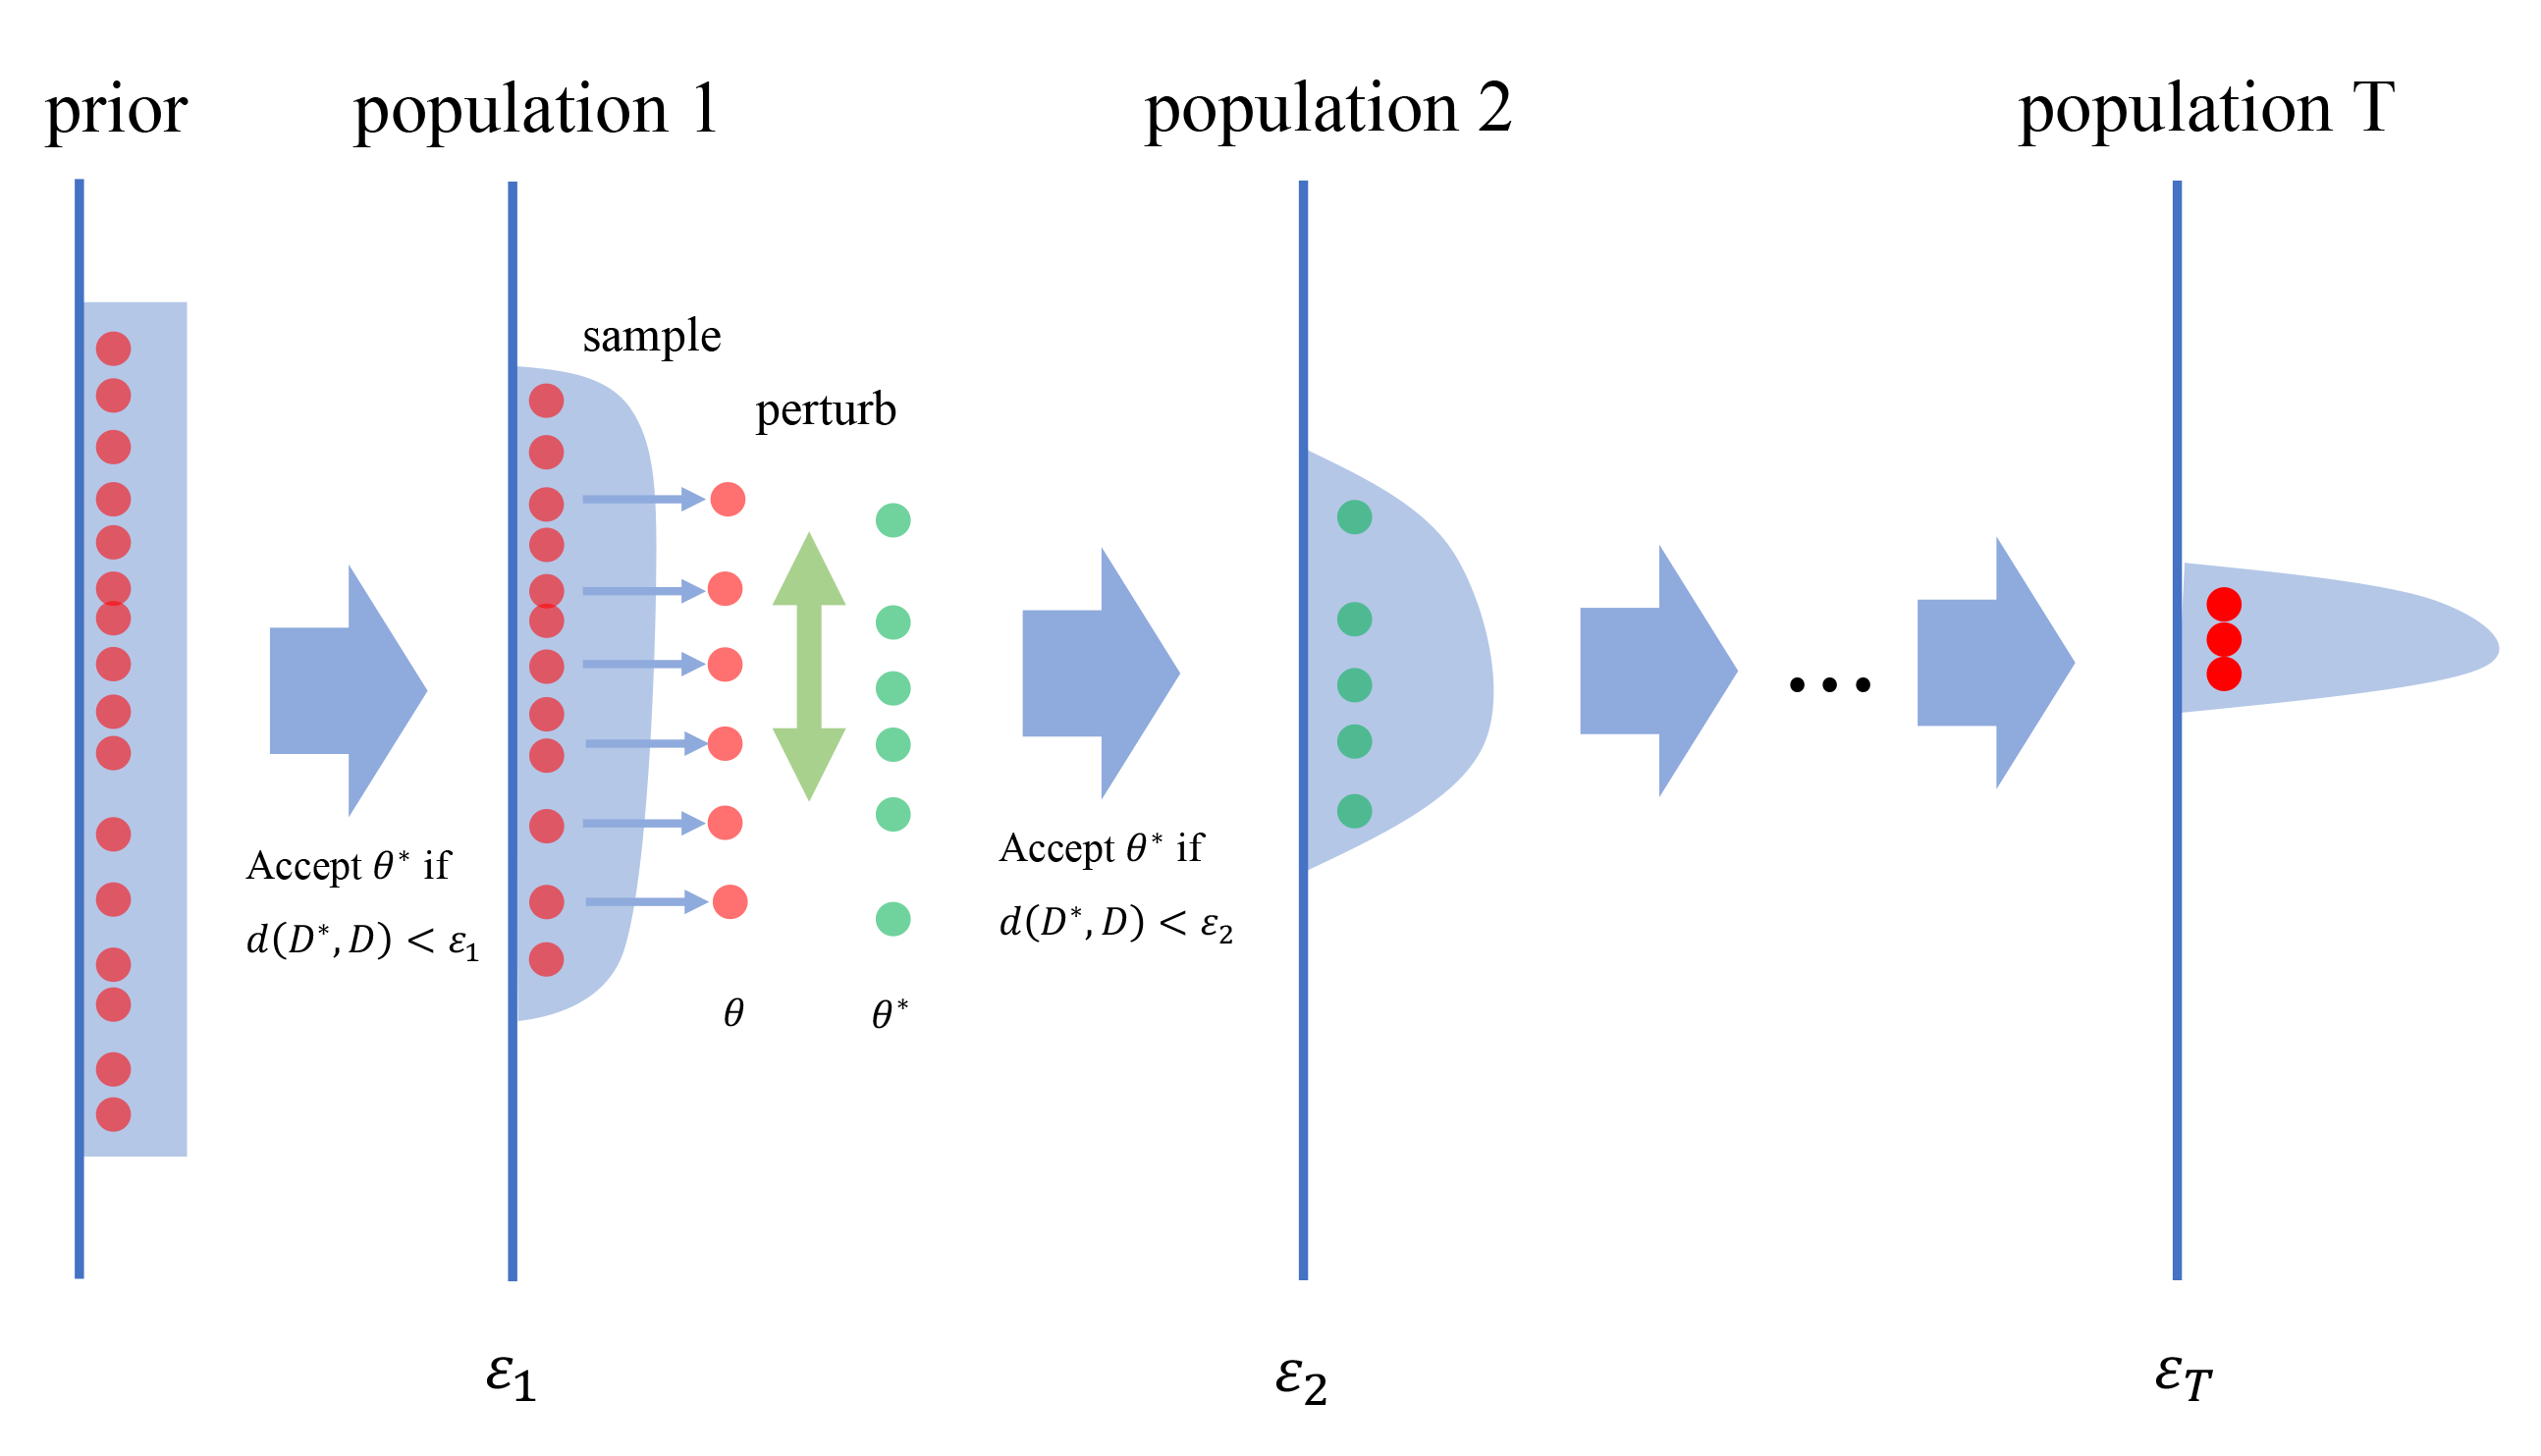
\includegraphics{fig/smc.png}}
    \end{center}

    \caption[ABC SMC sampling process]%
    {ABC SMC sampling process. $\theta^*$ denotes a sample drawn from previous population, which is used to generate simulated data $D^*$. $d$ is a distance measurement, $d(D^*,D)$ represents the discrepancy between observed data and simulated data. for each population $t$, $\epsilon_t$ is a threshold criterion to determine whether to accept that drawn sample}
    \label{fig:smc}

\end{figure}

In addition, ABC SMC is also capable of model selection tasks \cite{model_compare}. Instead of draw samples from prior of a single model, we can draw samples from multiple models $m_i$ and approximate $p(m_i, \theta|D)$, which is the joint probability distribution of model $m_i$ and its accepted particles $\theta$. In each generation the marginal distribution $p(m_i|D)$ can be calculated as the accepted ${\theta}$ is known, thus models can be ranked according to their probabilities.

The feature that ABC algorithm can perform likelihood-free inference makes it widely used in many dynamic modeling problems, especially in the area of biology \cite{ref:abcsysbio, ref:disease, ref:compare}. But ABC is not limited to these areas, as it can be generally used in inference tasks to give parameter estimates or model rankings. E.g., it has been successfully applied in cosmology studies \cite{cosmology}.



\section{Software tools}

%  [existing tools and software for this task]

%  [workflow and developing process]

 As we decided to apply ABC SMC on our regeneration models for its high-dimensional parameter estimation and comparison of different models, a code development and experiments workflow was expected to be built. The ABC SMC algorithm needs a whole set of mathematical environments (e.g. class of distributions, models and particles) and closely linked sampling and fitting algorithms (e.g. KDE fitting and Gaussian sampling), thus suitable platforms with related software packages are preferred. Regarding this, several packages in \verb|R| and \verb|Python| were studied.

 A software packages that integrally implement ABC SMC is preferred, and more options in the settings of the algorithm, more customisable features make it better. Moreover, as the ABC SMC itself is a computationally intensive task that contains massive parallel potentials, an ideal software package is expected to support as least one kind of parallel options e.g. multi-core, GPU accelerating and clusters. Otherwise, a modification or rewrite of the software package are expected to produce a reliable input-output framework for our parameter estimation and model selection experiments, where much more work would be introduced.

 Preliminarily \verb|pyABC| packages \cite{ref:pyabc} in \verb|Python| was chosen for implementations. \verb|pyABC| supports multiple types of parallelisation, e.g., multicore processing and distributed cluster, and supports resume stored runs, which made our experiments easier. It is well documented and flexible in customisations of the algorithm.

 Some other ABC SMC related packages were also examined and considered as backups, include ELFI \footnote{\url{https://elfi.readthedocs.io/en/latest/}}, ABC-SysBio \cite{ref:abcsysbio}, EasyABC\footnote{\url{https://cran.r-project.org/web/packages/EasyABC/index.html}}, GpABC \footnote{\url{https://github.com/tanhevg/GpABC.jl}}, etc. These packages may have their advantages (e.g. ABC-SysBio supports CUDA acceleration) and considered as alternative implementation methods, or can be used to compare performance difference.

 Additionally, some other softwares were also need for solving ODE, results analysis and visualisations. These software and hardware environments are listed in Appendix A.

\chapter{Mathematical modelling}

Mathematical models can describe different kinds of dynamic systems, and thus can be used in prediction, analysis and other tasks. An ideal model in our case, can represent reasonable interactions or effects between immune cells and cytokines and reproduce features and characteristics that were observed in experimental data.

Proposed models for the regeneration process were in the form of non-linear ordinary differential equations (ODE). The only independent variable is post-lesion time $t$. The equations consist of four derivatives of dependent variables (number of cells, mRNA expression of cytokines) with respect to $t$. The equations were mostly an interpretation of the proposed interaction maps, with terms correspond to interaction paths.


\section{Observed data}

Our models were built based on the existing experimental findings from Tsarouchas et al. \cite{ref:Tsarouchas}. The available measurement data included the numbers of three kinds of cells (neutrophil $N$, macrophage $\Phi$ and microglia) and the relative mRNA expression of four kinds of cytokines (il-1$\beta$, tnf-$\alpha$, tgf-$\beta$1a and tgf-$\beta$3). As proposed by Tsarouchas et al., neutrophil and macrophage play essential roles in controlling the il-1$\beta$ and tnf-$\alpha$ mediated inflammation. Our initial models focused on the changes of four dependent variables $N$, $\Phi $, $\beta$ (for il-1$\beta$) and $\alpha$ (for tnf-$\alpha$) that are most important and determinative in the regeneration. $N$ and $\Phi$ is of the unit `number of cells', $\beta$ and $\alpha$ is recorded as `relative mRNA expression' (compared to the value at the initial time point, i.e. 0 hpl) and considered unitless.

It was noted that the variance of the measured data is relatively high. The summary statistic was the mean of measurement data at each time point, assuming that measured data was Gaussian-like distributed. To validate this, the distribution of the measured data points was plotted. The result was that at most time points the measurement values are Gaussian-distributed, although some distributions were skewed. One abnormal distribution was observed at time point 120 hpl for macrophage where there are two concentrations. Despite this, the mean value could summarise most data and thus was still used as the target summary data. The mean value at each time point is shown in Figure \ref{fig:obs_data}, which is our target trajectories for the models to fit.

\begin{figure}
    \begin{center}
        \resizebox{1.0\hsize}{!}{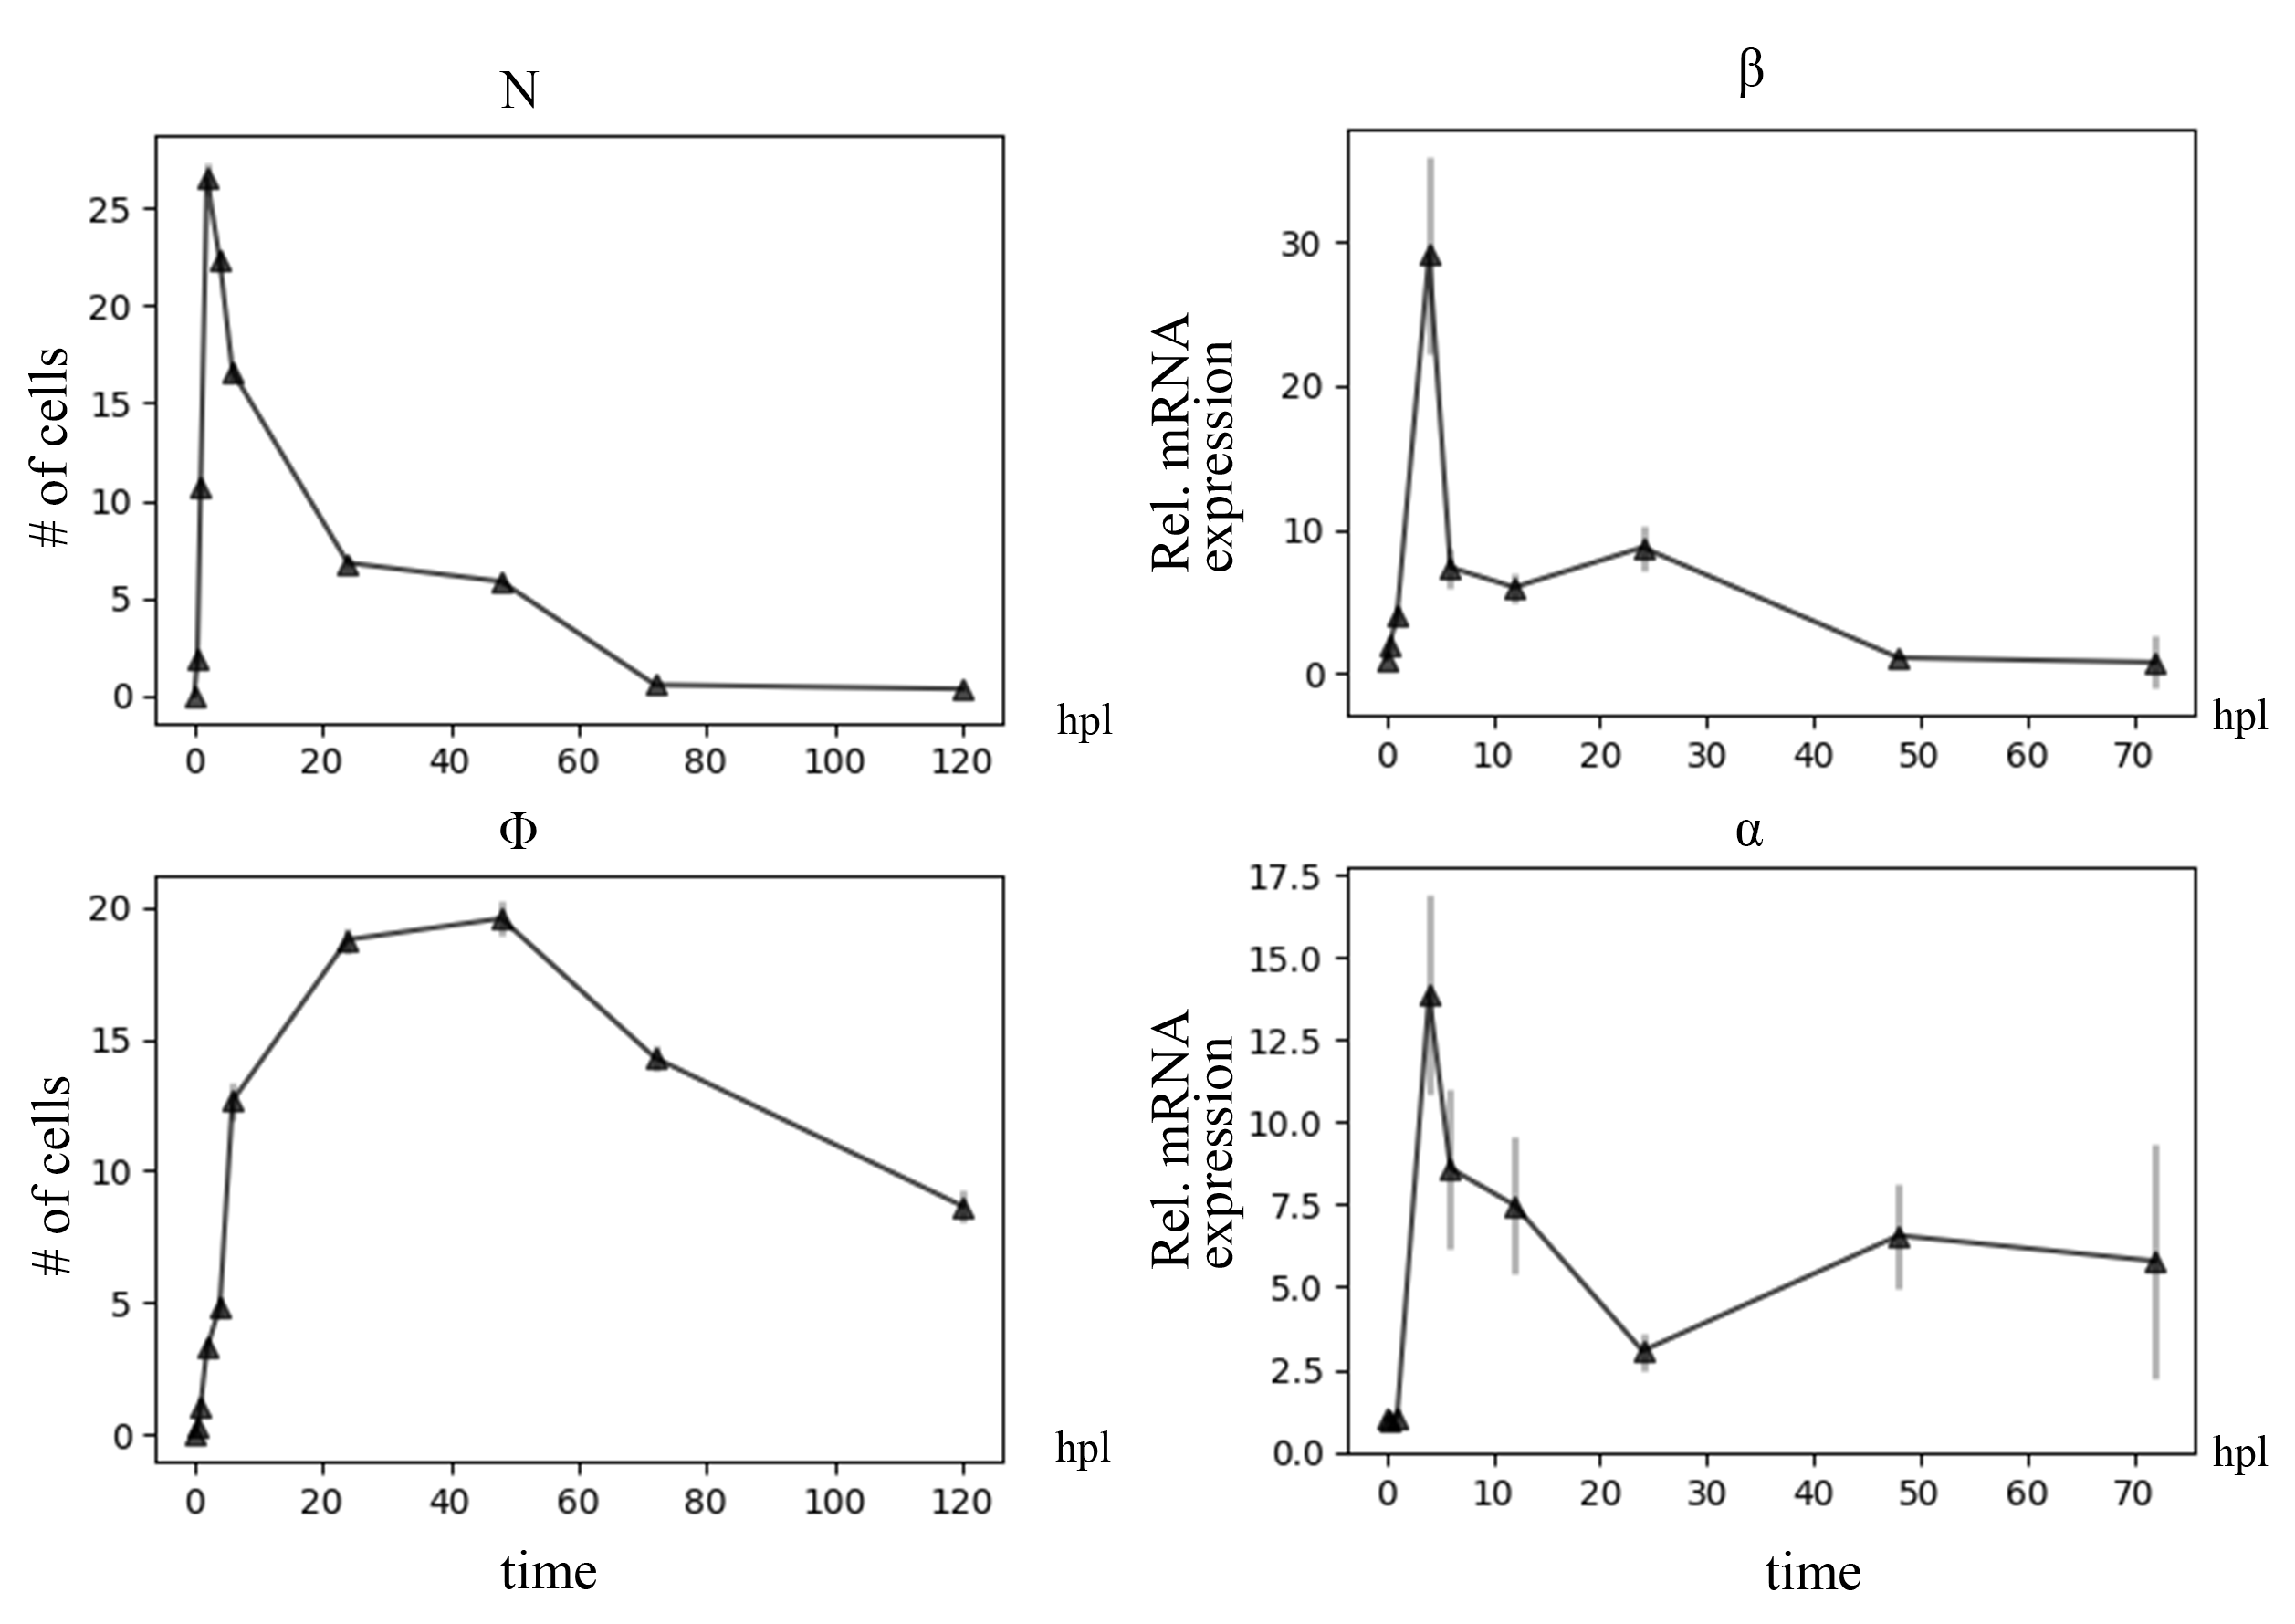
\includegraphics{fig/observed.png}}
    \end{center}

    \caption[Mean of the observed data]%
    {Mean of the observed data for neutrophil ($N$), macrophage ($\Phi$), il-1$\beta$ and tnf-$\alpha$, from experiment results of \cite{ref:Tsarouchas}. Error bars indicate standard error of mean (SEM). For $N$ and $\Phi$ the SEM is relatively small}
    \label{fig:obs_data}

\end{figure}

\section{Hypotheses and models}

Five models in total are proposed according to different hypotheses. At first, our tests and implementations of ABC SMC for parameter estimations used only the basic model for developing propose. After the parameter inference framework was built and tested, more models were proposed in order to calibrate and improve the basic model such that the observed regeneration process can be better represented.

All these models assumed that the involved interactions are within two kinds of cells (neutrophil and macrophage) and two kinds of cytokines (il-1$\beta$ and tnf-$\alpha$), and used the data presented in Figure \ref{fig:obs_data} for the inference task. Interactions or influences from other cells or cytokines are not considered as there might not be corresponding data available. If such data or experimental findings are available in the future, we can consider them by then as long as these interactions are indeed necessary for our model.

\subsection{Basic model}

A preliminary model (Eqn. \ref{eq:model1}) was proposed according to \cite{ref:Tsarouchas} and then mainly used to build and test the code of inference framework. An interaction map of the model is shown in Figure \ref{fig:m1}. This model is a simplification of the process described in \cite{ref:Tsarouchas} (Figure \ref{fig:map}) with some minor interactions ignored. This model included 12 parameters, all of which should be positive real numbers. A description of these parameters can be found in Table \ref{table:m1}.

\begin{figure}
    \begin{center}
        \resizebox{0.4\hsize}{!}{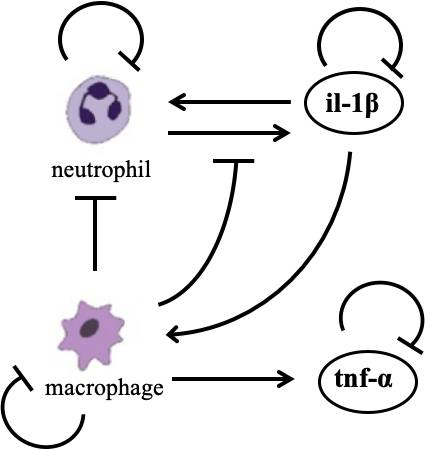
\includegraphics{fig/model1.png}}
    \end{center}

    \caption[Interactions modelled in the basic model]%
    {Interactions modelled in the basic model (model 1) based on Tsarouchas et al.\cite{ref:Tsarouchas}. Lines ended with arrow represent promoting effect, lines ended with T-connectors represent inhibition}
    \label{fig:m1}

\end{figure}
\begin{align}
    \label{eq:model1}
    \begin{split}
        &\frac{\mathrm{d} N}{\mathrm{d} t}=\lambda_N+\kappa_{N\beta}\beta-\mu_NN-\nu_{N\Phi}N\Phi\\
        &\frac{\mathrm{d} \Phi}{\mathrm{d} t}=\lambda_\Phi+\kappa_{\Phi\beta}\beta-\mu_\Phi\Phi\\
        &\frac{\mathrm{d} \beta}{\mathrm{d} t}=\frac{s_{\beta N}N}{1+i_{\beta\Phi}\Phi}-\mu_\beta\beta\\
        &\frac{\mathrm{d} \alpha}{\mathrm{d} t}=s_{\alpha\Phi}\Phi-\mu_\alpha\alpha
    \end{split}
\end{align}
It was assumed that there are negative feedbacks the cells and cytokines, i.e. overcrowding inhibits the increasing rates. As sources, macrophage produces tnf-$\alpha$ and neutrophil produces il-1$\beta$; however, macrophage was assumed to have a negative effect on the il-1$\beta$, term $1+i_{\beta\Phi}\Phi$ in Eqn. \ref{eq:model1} was used to represent this. Despite the self-driven increase of immune cells, il-1$\beta$ was assumed to promote the increase of both cells. Neutrophil was also assumed to be inhibited by the total immune cells presented in the lesion site, the term $\nu_{N\Phi}N\Phi$ was used to denote this.

\begin{table}[t]
    \centering
    \begin{tabular}{|c c c|}
        \hline
        Parameter            & Definition                                       & Units                    \\ [0.5ex]
        \hline\hline
        $\lambda_N$          & Self-increase rate of neutrophil                 & $cell/h$                 \\
        $\kappa_{N\beta}$    & Promoting effect coefficient by il-1$\beta$      & $cell/h$                 \\
        $\mu_N$              & Coefficient of negative feedback of $N$          & $h^{-1}$                 \\
        $\nu_{N\Phi}$        & Coefficient of inhibition of both $N$ and $\Phi$ & $cell^{-1}\cdotp h^{-1}$ \\
        \hline
        $\lambda_\Phi$       & Self-increase rate of macrophage                 & $cell/h$                 \\
        $\kappa_{\Phi\beta}$ & Promoting effect coefficient by il-1$\beta$      & $cell/h$                 \\
        $\mu_\Phi$           & Coefficient of negative feedback of $\Phi$       & $h^{-1}$                 \\
        \hline
        $s_{\beta N}$        & Production rate from $N$                         & $cell^{-1}\cdotp h^{-1}$ \\
        $i_{\beta\Phi}$      & Coefficient of inhibition to the production      & $cell^{-1}$              \\
        $\mu_\beta$          & Coefficient of negative feedback of $\beta$      & $h^{-1}$                 \\
        \hline
        $s_{\alpha\Phi}$     & Production rate from $\Phi$                      & $cell^{-1}\cdotp h^{-1}$ \\
        $\mu_\alpha$         & Coefficient of negative feedback of $\alpha$     & $h^{-1}$                 \\
        \hline
    \end{tabular}
    \caption{Parameters introduced in the basic model (model 1) [REMOVE unit]}
    \label{table:m1}
\end{table}

\subsection{Alternative models}

\paragraph{Model 2 and model 3}

As the observed data indicated, this dynamic system has a steady-state where after a long time ($\geq 120$ hpl), the inflammation is resolved, and immune cells should not be present at the injury site any more. Regarding this, the parameter for self-increase rate for the macrophage and neutrophil, i.e. $\lambda_\Phi$ and $\lambda_N$  cannot be constant. An exponentially decaying $\lambda$ term is introduced in the new model (model 2, Eqn. \ref{eq:model2}). Also, the inhibition of il-1$\beta$ production, i.e. the term $i_{\beta\Phi}\Phi$ is considered to be ignored for a more simple model, in which case the relative expression of il-1$\beta$ is only affected by the number of neutrophils and the negative feedback from itself. This case corresponds to model 3, written as Eqn. \ref{eq:model3}.

Model 2 and model 3 introduced one extra parameter $a$ and removed $\lambda_\Phi$, which is a coefficient in the exponentially decaying $\lambda_N$, determining the decay speed, with the unit $h^{-1}$.
\begin{align}
    \label{eq:model2}
    \begin{split}
        &\frac{\mathrm{d} N}{\mathrm{d} t}=\lambda_Ne^{-at}+\kappa_{N\beta}\beta-\mu_NN-\nu_{N\Phi}N\Phi\\
        &\frac{\mathrm{d} \Phi}{\mathrm{d} t}=\kappa_{\Phi\beta}\beta-\mu_\Phi\Phi\\
        &\frac{\mathrm{d} \beta}{\mathrm{d} t}=\frac{s_{\beta N}N}{1+i_{\beta\Phi}\Phi}-\mu_\beta\beta\\
        &\frac{\mathrm{d} \alpha}{\mathrm{d} t}=s_{\alpha\Phi}\Phi-\mu_\alpha\alpha
    \end{split}
\end{align}

\begin{align}
    \label{eq:model3}
    \begin{split}
        &\frac{\mathrm{d} N}{\mathrm{d} t}=\lambda_Ne^{-at}+\kappa_{N\beta}\beta-\mu_NN-\nu_{N\Phi}N\Phi\\
        &\frac{\mathrm{d} \Phi}{\mathrm{d} t}=\kappa_{\Phi\beta}\beta-\mu_\Phi\Phi\\
        &\frac{\mathrm{d} \beta}{\mathrm{d} t}=s_{\beta N}N-\mu_\beta\beta\\
        &\frac{\mathrm{d} \alpha}{\mathrm{d} t}=s_{\alpha\Phi}\Phi-\mu_\alpha\alpha
    \end{split}
\end{align}
Model 3 can be regarded as a simplification of model 2, as it can be treated as model 2 with parameter $i_{\beta\Phi}=0$. Among the proposed three models, model 1 is a naive one that was proposed at the very first time and used as an ODE `template' to build and test our parameter inference framework. As the implementation was successful, model 2 and 3 was proposed, as we were trying to calibrate some terms and find better models. After fitting, model 2 is supposed to be better than model 1 as it corrects the problem that appears at the final time points (which were related to the steady states of immune cells). Model 3 made a small simplification based on model 2, and thus it was theoretically less `general' than model 2.

\paragraph{Model 4 and model 5}

After the first model selection experiment among the exiting three models, it was found that any of the models did not recover some significant features presented in the observed data. To resolve this, attempts were tried to introduce additional reasonable interactions within the dynamic system, considering the biological and mathematical context. Extra promoting effect to the expression of tnf-$\alpha$ was considered, by either adding a phenomenological term $d_{\beta\alpha}\beta$ (which means the same effect as directly promoting but the underlying mechanism is unclear), or adding a term $f_{\beta\alpha}$ that represents a promoting effect to the production process of tnf-$\alpha$, namely model 4 (Eqn. \ref{eq:model4}) and model 5 (Eqn. \ref{eq:model5}).
\begin{align}
    \label{eq:model4}
    \begin{split}
        &\frac{\mathrm{d} N}{\mathrm{d} t}=\lambda_Ne^{-at}+\kappa_{N\beta}\beta-\mu_NN-\nu_{N\Phi}N\Phi\\
        &\frac{\mathrm{d} \Phi}{\mathrm{d} t}=\kappa_{\Phi\beta}\beta-\mu_\Phi\Phi\\
        &\frac{\mathrm{d} \beta}{\mathrm{d} t}=s_{\beta N}N-\mu_\beta\beta\\
        &\frac{\mathrm{d} \alpha}{\mathrm{d} t}=s_{\alpha\Phi}\Phi-\mu_\alpha\alpha+d_{\beta\alpha}\beta
    \end{split}
\end{align}

\begin{align}
    \label{eq:model5}
    \begin{split}
        &\frac{\mathrm{d} N}{\mathrm{d} t}=\lambda_Ne^{-at}+\kappa_{N\beta}\beta-\mu_NN-\nu_{N\Phi}N\Phi\\
        &\frac{\mathrm{d} \Phi}{\mathrm{d} t}=\kappa_{\Phi\beta}\beta-\mu_\Phi\Phi\\
        &\frac{\mathrm{d} \beta}{\mathrm{d} t}=s_{\beta N}N-\mu_\beta\beta\\
        &\frac{\mathrm{d} \alpha}{\mathrm{d} t}=(s_{\alpha\Phi}+f_{\beta\alpha}\beta)\Phi-\mu_\alpha\alpha
    \end{split}
\end{align}
\begin{table}[h!]
    \centering
    \begin{tabular}{|c c c|}
        \hline
        Parameter         & Definition                                                     & Units                    \\ [0.5ex]
        \hline\hline
        $d_{\beta\alpha}$ & Coefficient of promoting effect from $\beta$                   & $h^{-1}$                 \\
        \hline
        $f_{\beta\alpha}$ & Coefficient of promoting the production of $\alpha$ by $\beta$ & $cell^{-1}\cdotp h^{-1}$ \\
        \hline
    \end{tabular}
    \caption{Parameters introduced in model 4 and 5}
    \label{table:m45}
\end{table}



% \subsection{Model evaluation and comparison}

% [general topics on evaluating a model]

% There exists several metrics to evaluate the model based on the observed data. A widely used method is to simulate the data from the model, then calculate the discrepancy between simulated data and observed data. P-norm distance functions are usually used in this method

% [bayes factor for model selection]

\subsection{Limitations}

% [hypothesis]

% [available data]

% [model misspecification]

Some limitations were included in Section 3.1, where the observed data have a relatively high standard deviation at certain measurement points. More measurement repeats or more measurement points could help to represent more accurate trajectories of the modelled variables, and thus more possible models can be proposed. On the other hand, more accurate observed data are always beneficial to mathematical modelling, especially to complex dynamic systems.

As stated, our models are largely based on the experimental evidence from Tsarouchas et al.\cite{ref:Tsarouchas}. Some hypothesised interactions may differ from a real case, and there may exist undiscovered mechanisms. These could lead to model misspecification, where the model could fit the data but with wrong interaction paths, or the model can hardly fit the data and recover some local features observed in the data.

% \begin{figure}

% \begin{center}
% \resizebox{0.30\hsize}{!}{
\includegraphics{logos/crest_bw}}
% \end{center}

% \caption{The University Crest}
% \label{fig:eucrest}

% \end{figure}


% see the man page for dvips for details of the special command which is
% much more powerful than is shown here. It allows offsets in the
% horizontal and vertical and scaling in x and y.

% choosing suitable values for offset and scale can be a tiring matter
% of trial and error.

% note that labels do not need to include a description of the object
% they are labelling but it can be helpful, eg \label{fig:figurename}.

% You can use a label on a figure to refer to it later. The university
% crest is in \ref{fig:eucrest}. Note that you should not use phrases like
% ``the figure above'' or ``the following figure'' since Latex may move
% the figure relative to the text if it cannot be fitted onto the current page.








\chapter{Parameter estimation and model comparison}

For the proposed models, exploration of the uncertainties in the parameter estimations is our main task in this chapter, which involved the application of ABC SMC and several experiments. After that, the parameter inference framework was also used for model selection.

The build and test of the code were under \verb|Python| environment with \verb|pyABC|\cite{ref:pyabc}. Some other code, e.g. shell scripts and \verb|R| code were also used to perform the experiments and result analysis. Software and system environment used in our implementation can be found in Appendix A. The build and test were performed on local computers and HPC facilities available within EPCC.

\section{Code and implementations}

%  [ABC implementations details, e.g. distance, population, ODE related functions]

%  [how the code is developed and built]

According to our preliminary studies, a ABC SMC framework implemented using \verb|pyABC| in \verb|Python| was adopted in this project. \verb|pyABC| is a popular SMC software packages\cite{ref:pyabc} which has been used form many ABC SMC inference applications\cite{population}. \verb|pyABC| provides an open-source framework for likelihood-free inference, which is a \verb|NumPy| implementation of ABC SMC algorithm and a useful tool-box for our own inference and analysis tasks. Besides, it supports multi-core execution implemented using \verb|multiprocessing| built-in package, and it made our further studies in the scaling-up performance possible.

%  which is of our interests and suitable for the followed performance experiments.

The inference framework code for the project was developed and tested in local environment (macOS 10.15.6, see Table \ref{table:local_macine}) at first using a small input, then the functional version was deployed on compute node of ARCHER and Cirrus for parameter inference experiments and model selection tasks. The scaling-up experiment was performed on Cirrus. The profiling and its analysis were performed on local machine. Some necessary development and debug were performed on the remote machines to ensure that experiments run correctly on compute node.

The ODE model-related code and utilities were firstly developed to enable reusable functions, variables and data calls. It included the code for the ODE equations, ODE solver, data structures and data format transform functions, etc. By doing this in separate code files, we could change implementation options and activate ABC SMC easily in another `trigger' file, without creating definition and duplicated code for the models, observed data and parameter priors.

Some missing features were found when using \verb|pyABC|, therefore some modifications were made to the source code of \verb|pyABC|.

For example, the laboratorial measured data were not considered `complete' or `tidy' for modeling and analysis purpose: the available time points for cells and cytokines were different, e.g. cell number was not measured at 0.25 hpl and cytokines' expression was not measured at time point 120 hpl. These missing values were treated as `ignored' when calculating the distance between observed data and simulated data, and represented by \verb|NaN|s. However, in some distance calculations \verb|NaN| was not acceptable; to cope with this, built-in distance function was modified. Other modified code include some visualisation and result representation enhancements

Analysis of the program output was also wrapped up into functions which can be easily called after an ABC SMC run is finished, which includes multiple visualisations and summary statistic of the results. For different tasks there are also separated analysis code file. Other analysis tools used in the project include built-in database visualisation tool, R code and Microsoft Excel.

The project code was managed via \verb|git| version-control and available as a GitHub repository\footnote{\url{https://github.com/chaolinhan/MSc_Project}}; it also made the cross-hardware synchronisation of code versions convenient.

After several development iterations, code files for ABC SMC implementation now mainly had two types: code files for infer-back experiments (using synthetic data), and code files for parameter inference (using experimental data). Model selection can be easily done by adding more model to the implementation code file.


% \section{Parameter estimation}

% [implementation details and options/ settings that are affecting the ABC]





\section{Hyperparameters and implementation options experiments}

As the key focus of this project was on the parameter estimations of dynamical system, the ability of inference on the proposed models was firstly examined before actual inference using the experimental observed data.

In the first part, synthetic data is used with known true parameter values. The algorithm implementation is evaluated by the efficiency and goodness of resultant model under different implementation options and ABC SMC hyperparameters.

Then according to findings in the first part, several options with good performance are tried in the inference using experimental observed data (Figure \ref{fig:obs_data}). To obtain a more accurate and general results, these experiments are repeated for 3 or more times.

    % [including the options that are tested/ tried/ not adopted]

    % [including experiments results and discussions]

    % [how do these options correspond to biological model and how to set them accordingly for proposed model]

    % [why use synthetic data]

The ABC SMC inference can have largely different performance when using different hyperparameters and implementation options. To firstly test the ability of inference and observe the results of different options, synthetic data with known true parameter values are used as target data. by doing this, we could directly compare the inferred parameters to the true value, and compare the simulated trajectories to the true trajectories and then observe the result to see whether the inference is successful and how well the model fit the data. Also, by setting the same final threshold value, the efficiency under different options can be compared and help us to choose proper options when applying ABC SMC on the observed data. The true value of parameters that were used to generate synthetic data is listed in Table \ref{table:known_values}. 

The true values were obtained by fitting model 1 onto the experimental data (Figure \ref{fig:infer_back_data}) using least-square optimisation method. Available least-square fit tools in \verb|SciPy| were used. The fit algorithm was Trust Region Reflective\footnote{\url{https://docs.scipy.org/doc/scipy/reference/generated/scipy.optimize.least_squares.html}}. Target data was then generated using these parameter values via ODE integrate solver\footnote{\url{https://docs.scipy.org/doc/scipy/reference/generated/scipy.integrate.odeint.html}}.


\begin{figure}[ht]
    \begin{center}
        \resizebox{1.0\hsize}{!}{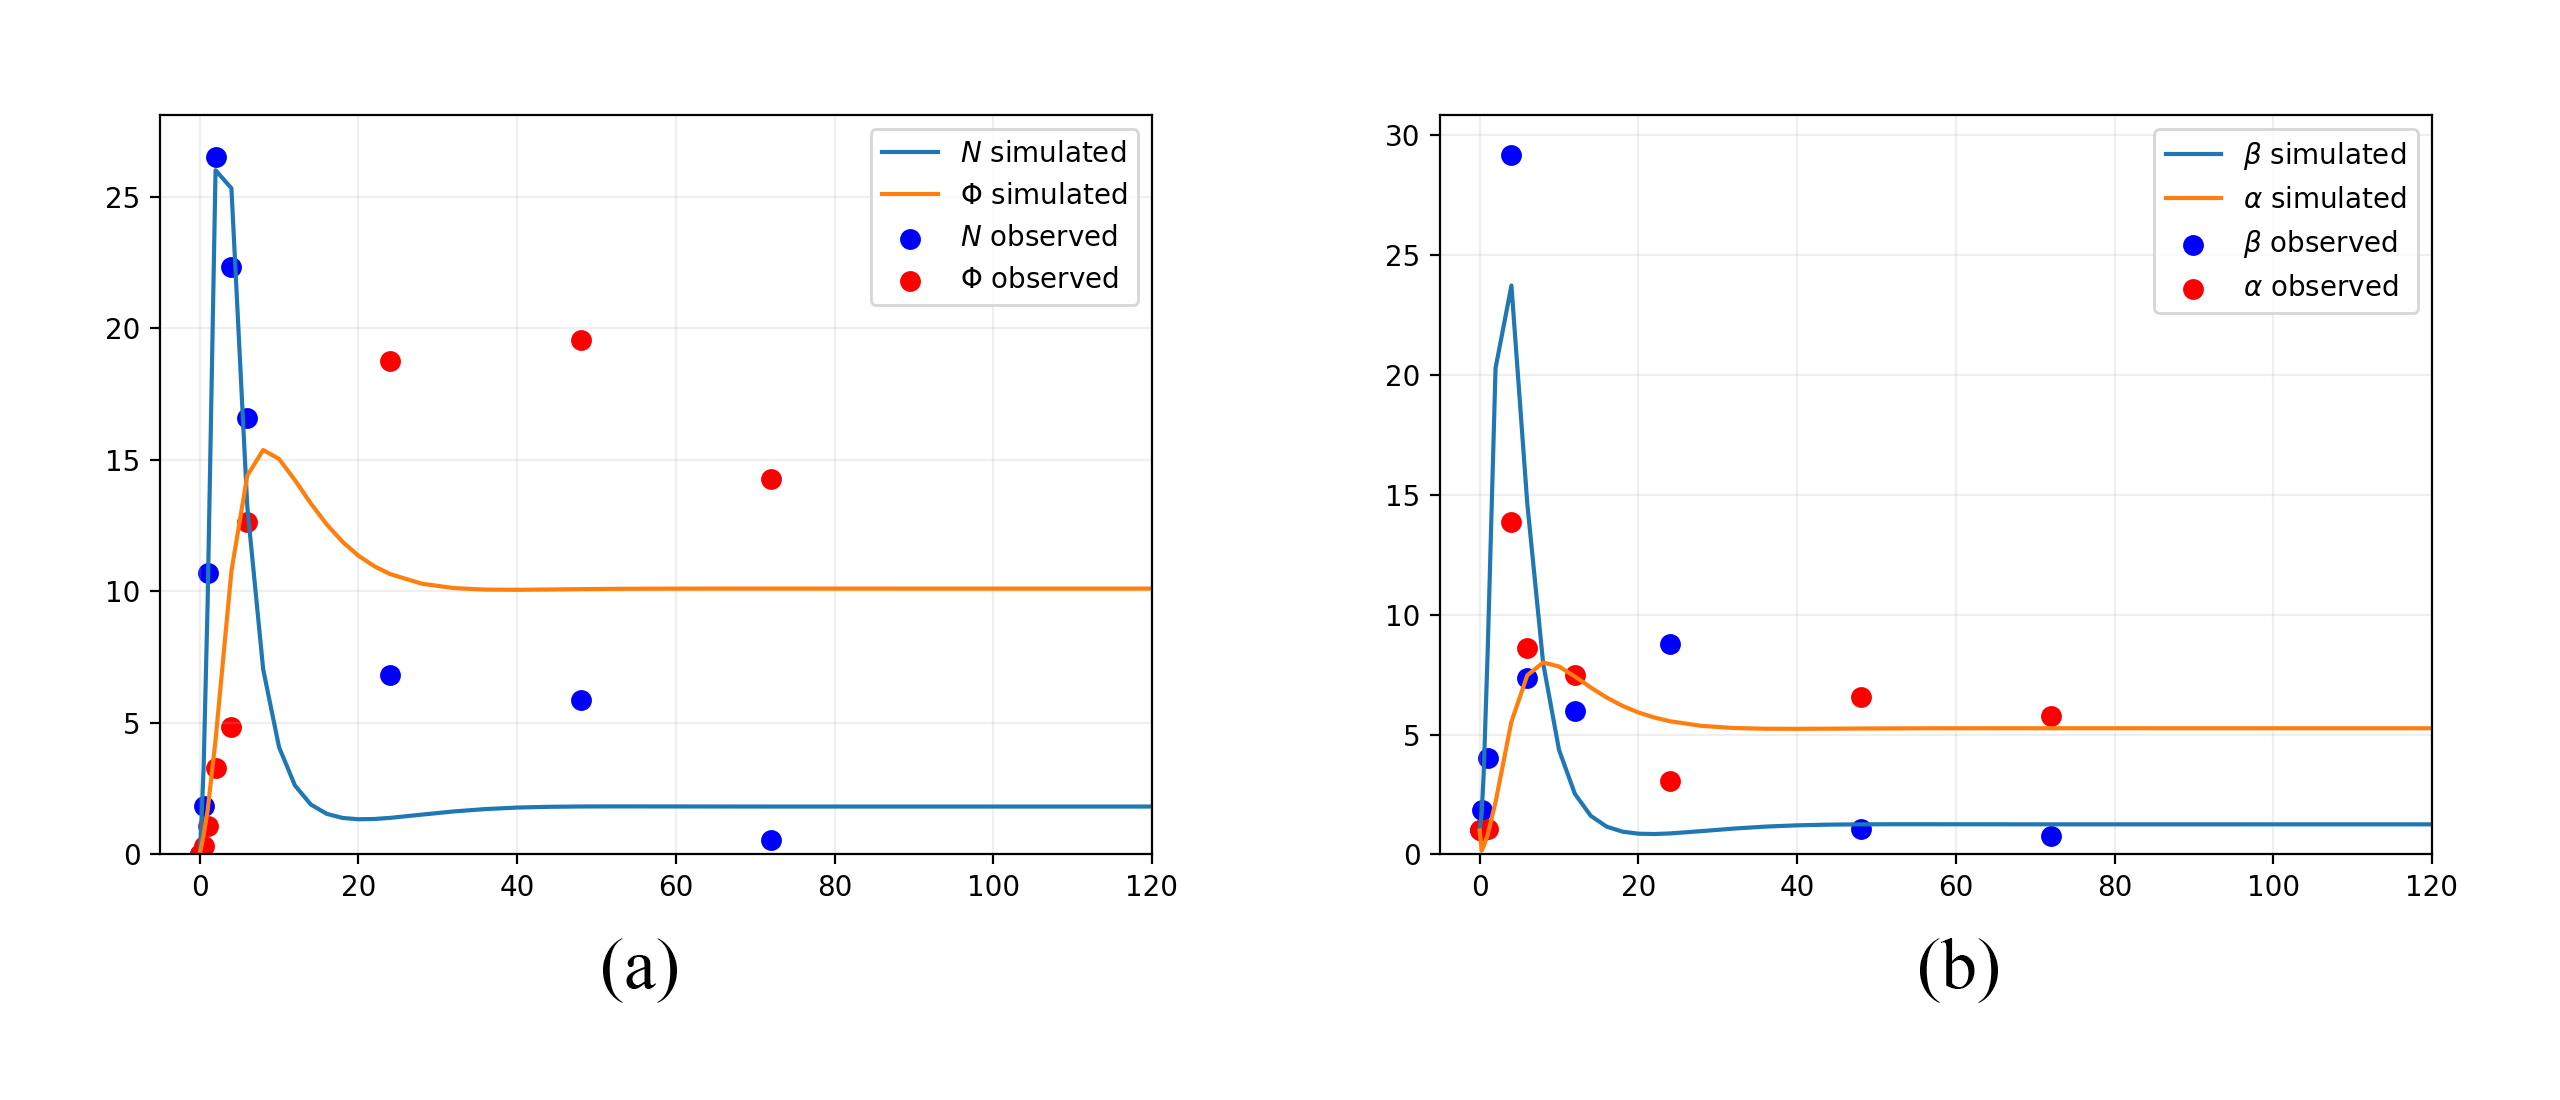
\includegraphics{fig/LS.png}}
    \end{center}

    \caption[Synthetic data generated with known parameter values]%
    {Synthetic data generated with known parameter values (line plot), compared to experimental data (scatter plot). Known parameter values are obtained from a least square fitting of the observed data}
    \label{fig:infer_back_data}

\end{figure}


The following topics were studied using the synthetic data and ABC SMC inference framework.

\subsection{Perturbation kernels}

Perturbation kernels work in the sampling process. In each generation $t$, samples are firstly taken from the previous population $\{\theta_{t-1}\}$ with weights $\{w_{t-1}\}$, then perturbed using the perturbation kernel $K(\theta|\theta^*)$. We keep sampling until $N$ particles are accepted, where $N$ is the pre-set population size. After that the new weights are calculated and normalised. Figure \ref{fig:smc} illustrates the process.

% \begin{figure}[t!]
%     \begin{center}
%         \resizebox{1.0\hsize}{!}{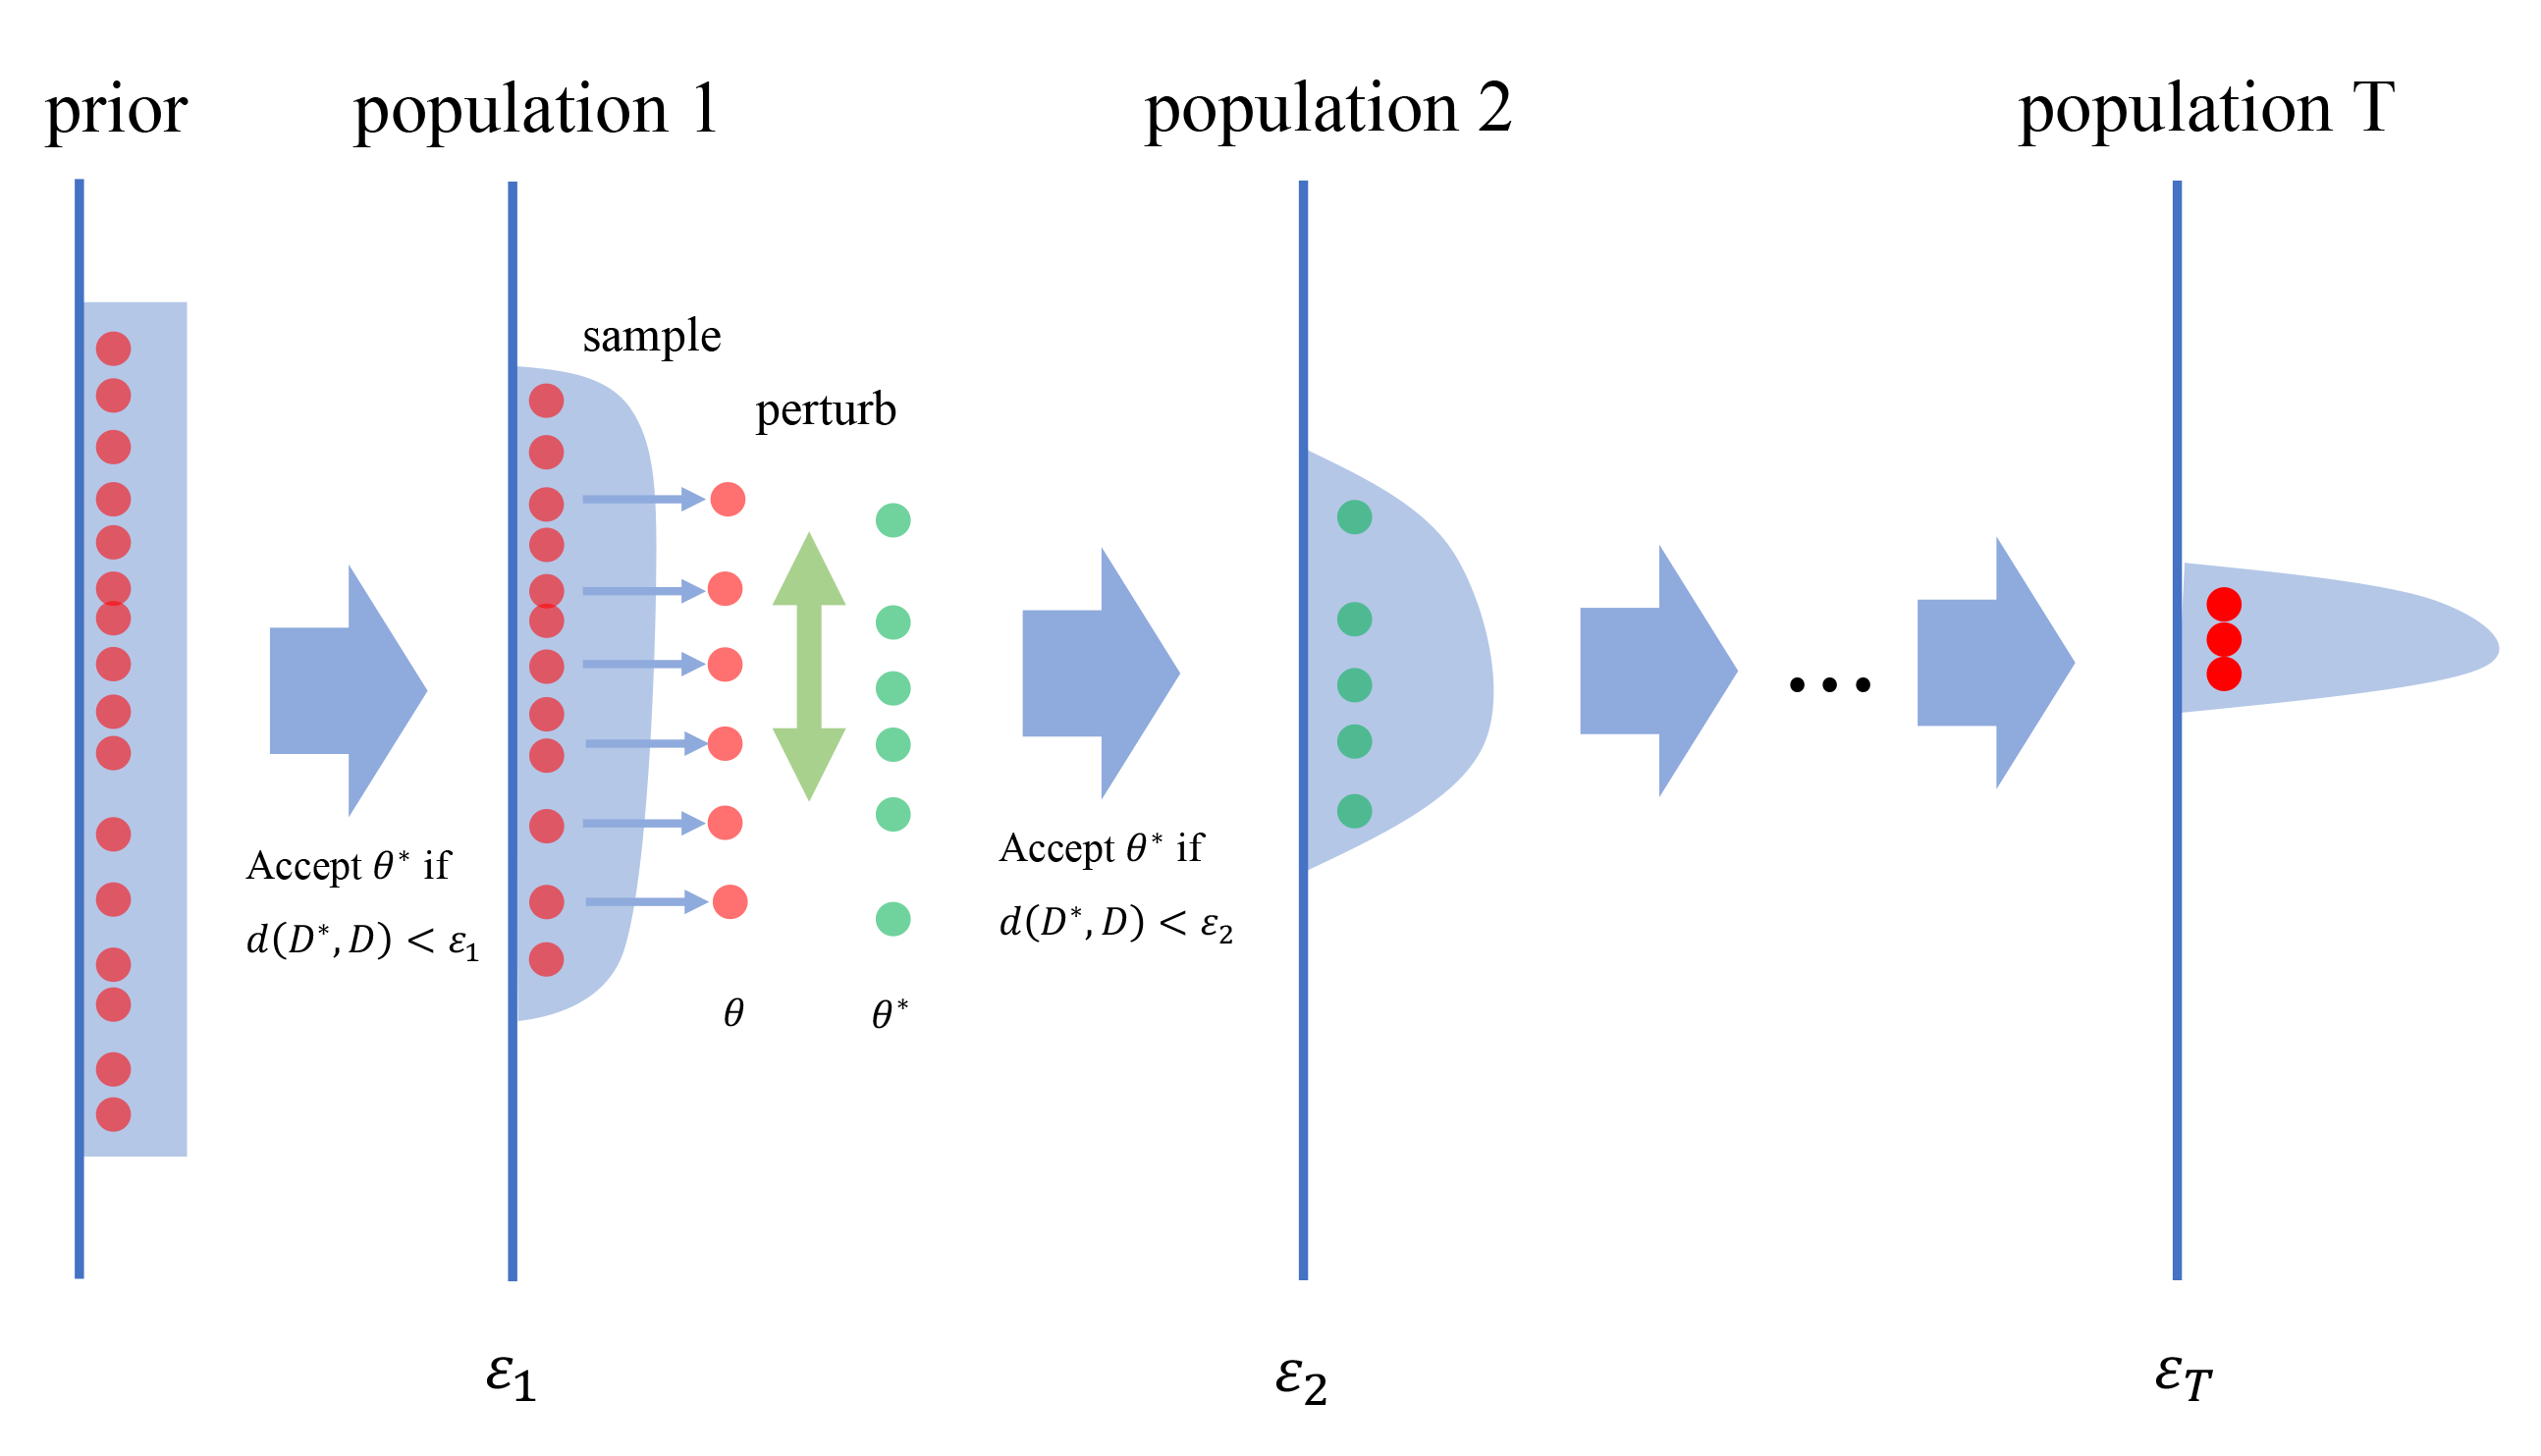
\includegraphics{fig/smc.png}}
%     \end{center}

%     \caption[ABC SMC sampling process]%
%     {ABC SMC sampling process. $\theta^*$ denotes a sample drawn from previous population, which is used to generate simulated data $D^*$. $d$ is a distance measurement, $d(D^*,D)$ represents the discrepancy between observed data and simulated data. for each population $t$, $\epsilon_t$ is a threshold criterion to determine whether to accept that drawn sample}
%     \label{fig:smc}

% \end{figure}

The perturbation kernel is called in the sampling of every particles and determines how the new perturbed particle is chosen, thus it is influential to both computation complexity and the resultant posterior distribution. Generally, a local perturbation kernel may face the risk of being stuck in local modes (e,g., local optimal), but it may need less computational operations, or could generate a population with a higher acceptance rate if the successive epsilon values are close; A kernel with wide variance, or spreading out in a large space could help in resolving the local optimal problem by a more thoroughly exploration of the parameter space, however it can be more computation-intensive and result in a lower acceptance rate. A desired optimal kernel should balance the trade-offs; their property and criteria is discussed in \cite{ref:kernel}.

There are several common choice of perturbation kernels. Among them multivariate normal kernel and local M-nearest neighbour model is preferred to be applied on our models. A covariance matrix $\Sigma_t$ of accepted particles is calculated form previous generation and used in multivariate normal kernel: $K(\theta|\theta_{t-1})\sim\mathcal{N}(\theta_{t-1}, \Sigma_t)$. It is illustrated to be more efficient than uniform kernel and component-wise normal kernel in relecting the true posterior structure \cite{ref:kernel}. It has been proved to perform well in several dynamic system models \cite{ref:abcsysbio, ref:compare, ref:disease} for the parameter estimation and model selection tasks. The $scaling\in(0,1]$ parameter in \verb|pyABC| will be multiplied to the covariance to produce a `narrower distributed' perturbation result.

Local M-NN kernel provided by \verb|pyABC| is also tried to provide a comparison. A local kernel density estimation (KDE) fit is used with M nearest neighbours considered.

The kernel experiments is designed to explore the efficiency of SMC on our dynamical systems. Given the same fixed threshold schedule, kernels that need less total samples and have higher acceptance rate would be our preference. The experiments compared multivariate normal kernel with local MNN kernels with different parameters, using synthetic data to infer back the parameters. The acceptance rate among each time point and total required samples are compared after the experiment to give suggestions on the kernel selection in the real data inference. As the threshold schedule is fixed, the final population should have similar discrepancy to the target data thus here the goodness of fit i.e. recover of target data trends/features and errors of the inferred parameters compared to true values is not discussed.

\subsubsection{Kernel experiment results}

To compare kernels, a fixed schedule schedule is used with minimal epsilon i.e. $\epsilon_t$ set to 10.0. From the total required samples graph Figure \ref{fig:kernel1}, the efficiency can be compared. Among the tested kernels, the local M-NN with M=50 has the best performance: it requires the least number of samples and
has higher acceptance rates among almost all generations. Local M-NN with M=750 is the slowest kernel.

For local M-NN kernels, generally a greater M will lead to lower acceptance rate and
more required particles in each generation. As shown in Figure \ref{fig:acceptance1}, local M-NN with M=750 is the lowest curve. Consequently, if greater M is test, then it will have even lower acceptance rates; the maximum M=2000 (whole population is considered) will have the lowest acceptance rates.

\begin{figure}
    \begin{center}
        \resizebox{1.0\hsize}{!}{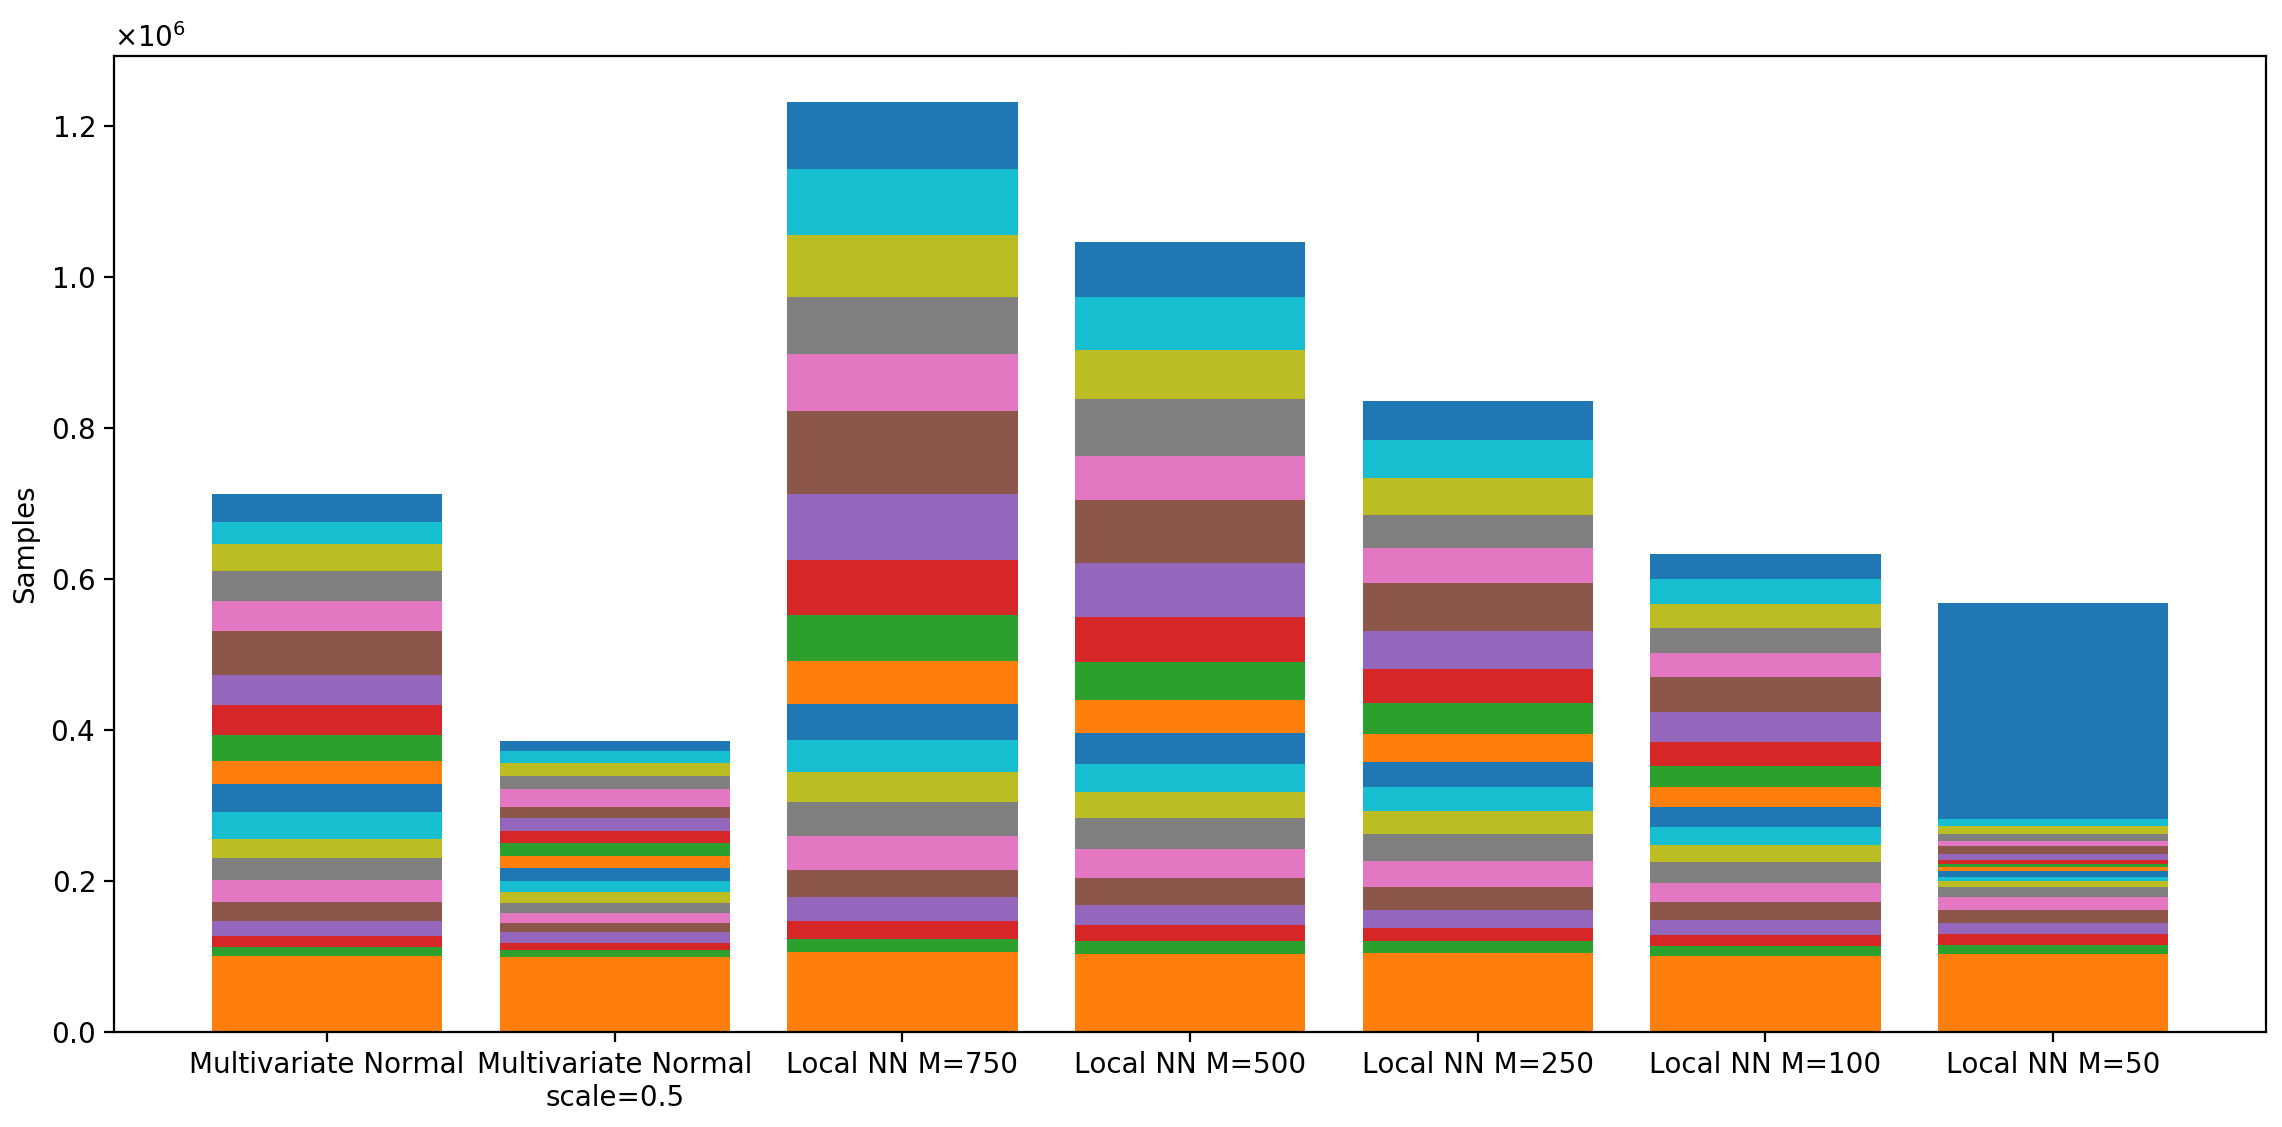
\includegraphics{fig/kernel1.png}}
    \end{center}

    \caption[Total required samples of different kernels]%
    {Total required samples of different kernels after 20 populations (2000 particles in each population). Different color represents different generations (bottom to top: population 1 to population 20)}
    \label{fig:kernel1}

    \vspace*{\floatsep}

    \begin{center}
        \resizebox{1.0\hsize}{!}{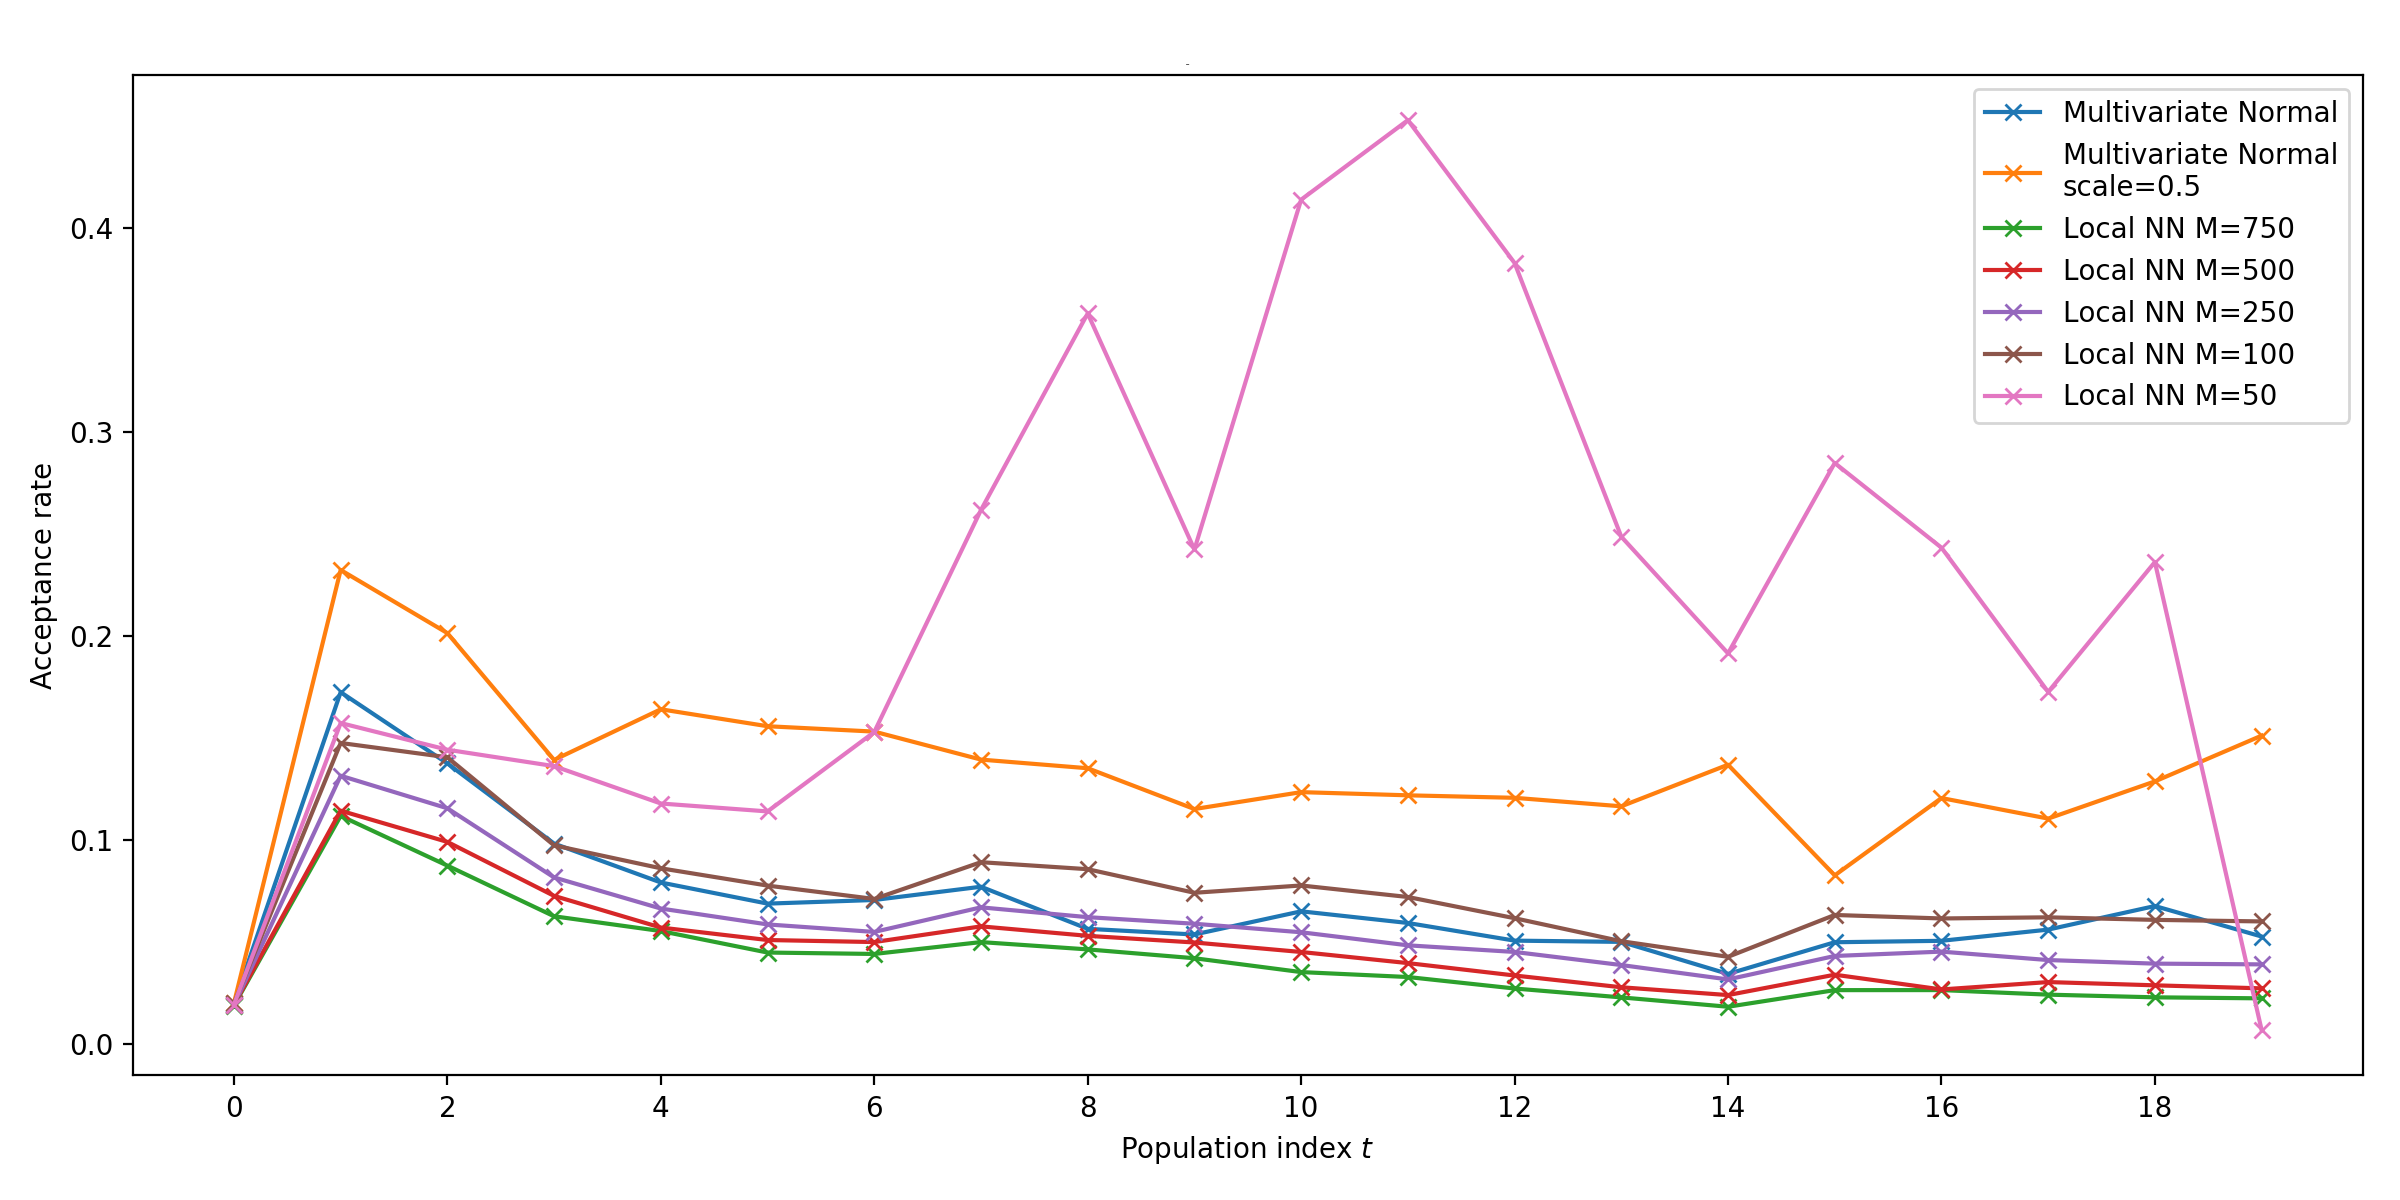
\includegraphics{fig/acceptance1.png}}
    \end{center}

    \caption[Acceptance rates of different kernels]%
    {Acceptance rates of different kernels in 20 populations. Each population has 2000 particles}
    \label{fig:acceptance1}

\end{figure}

Multivariate normal kernel has a performance between local M-NN M=250 and M=100. It proves that rather than a trivial normal kernel, multivariate normal kernels is more efficient facing the concentrations of joint distributions among multiple parameters \cite{ref:kernel}. `Scaling' option can narrower the distribution calculated from the last population, thus making the kernel more `local' by sampling under a smaller variance. Similar to small M in local M-NN, small `scaling' is also more efficient in our experiment of the model 1. Besides the fixed threshold schedule, a median threshold schedule with the same final threshold $\epsilon_{20}=10.0$ is also tested and similar results are observed (Figure \ref{fig:kernel2} and \ref{fig:acceptance2}, Appendix B2).

A more `local' kernel was more likely to give better performance by efficiently sampling around concentrations in parameters' distribution and approximate the posterior distribution. This holds in most cases under a given target final threshold value $\epsilon_t$, however may not produce the proper result want: a more local kernel, e.g. local M-NN with small M and multivariate normal with `scaling' is more likely to be stuck in local optimality, as the kernel is less likely to sample particles that are far from local concentrations, although these local optimal are still accepted under given threshold. In other words, using local kernels the epsilon may quickly converge to to local optimal; if a even smaller epsilon is desired, the local kernel can hardly generate enough particles to find another matched local modes. Also, the shapes of posterior distribution will affect the performance of local kernels \cite{ref:kernel}. One obvious example is presented in Figure \ref{fig:kernel1}, where local M-NN with M=50 suffered from a local optimal: the last generation takes much more samples to meet the required threshold.

\subsubsection{Conclusion} Local kernels can be fast bur unstable in some case; for a general parameter inference of our models, multivariate kernels are preferred, as a good fit is our prior target; some local kernels are also worth trying after the multivariate normal kernel, e.g. local M-NN with M$\leq 250$ (for population size of 2000, i.e. 12.5\% of the population) and multivariate normal with scaling. Also, multivariate M-NN is worth trying, although it was not built in \verb|pyABC| and requires additional implementations.


% \begin{figure}
%     \begin{center}
%     \resizebox{1.0\hsize}{!}{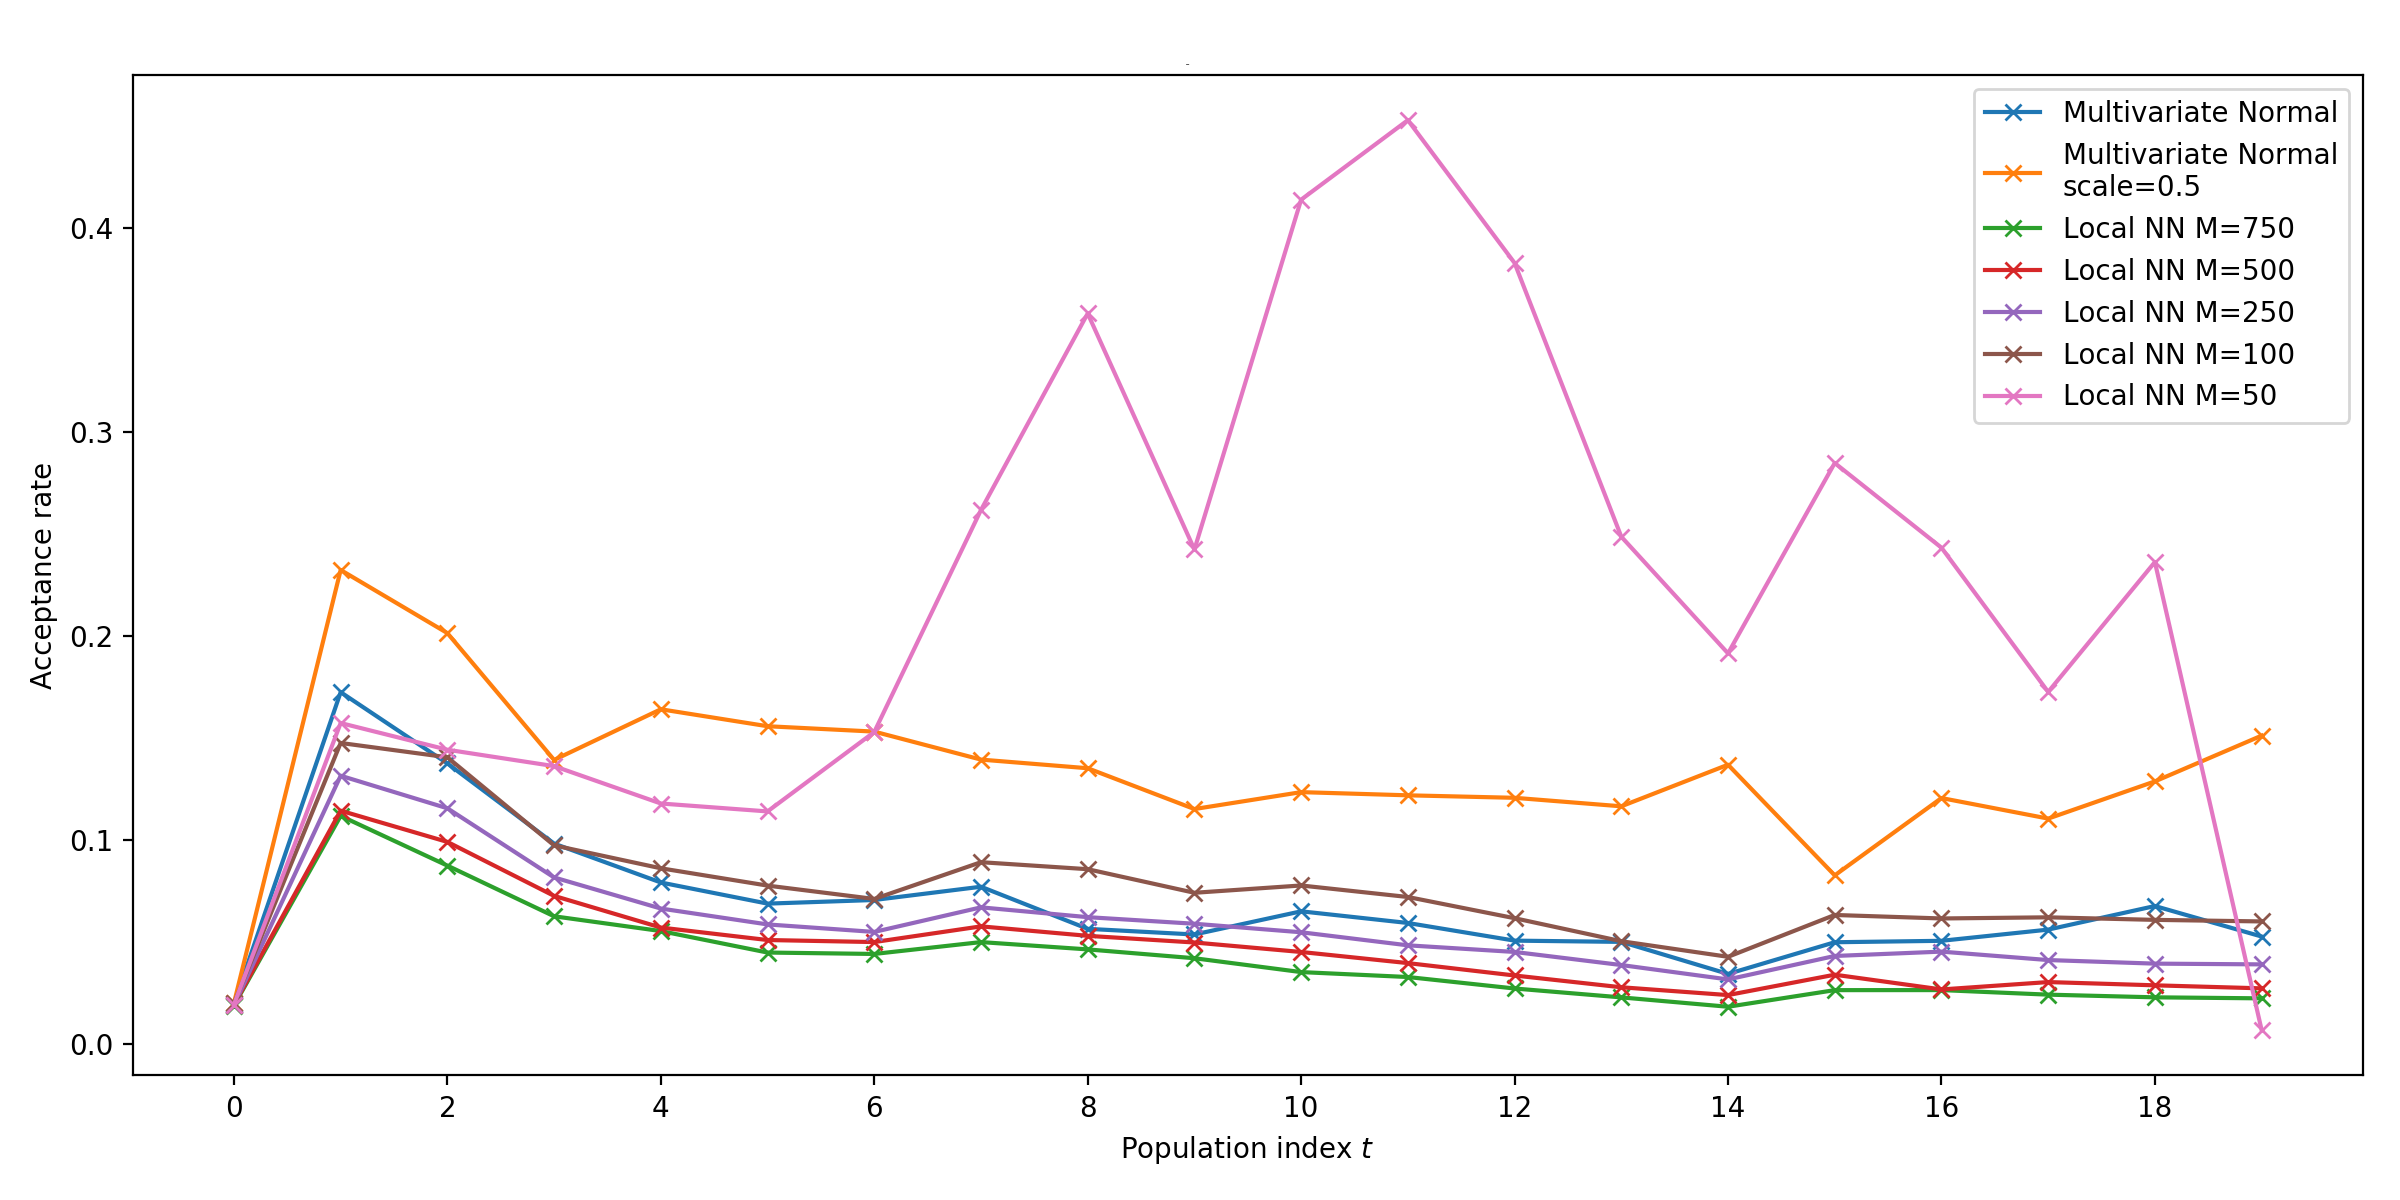
\includegraphics{fig/acceptance1.png}}
%     \end{center}

%     \caption{Acceptance rates of different kernels}
%     \label{fig:acceptance1}

% \end{figure}


\subsection{Adaptive functions and factors}

% [how adaptive distance work]

SMC can be more adaptive by introducing adaptive distance function and adaptive population; besides, factors can be applied to manually `normalise' the data.

The trivial distance function is set to Euclidean distance (2-norm distance)

\begin{align}
    \label{eq:dis}
    D=\sqrt{\sum_i \Delta x_i^2}
\end{align}

where $i$ is the index of data points and $\Delta x_i$ is the discrepancy between  observed data and simulated data at data point $i$, i.e. $\Delta x_i = x_{i, simulated}-x_{i, observed}$. In this case data points are 12 time points of four variables i.e. 48 data points in total.

A weighted 2-norm distance can be written as

\begin{align}
    \label{dis_w}
    D=\sqrt{\sum_i w_i \Delta x_i^2}
\end{align}

where a weight $w_i$ is assigned to every data point. If data point $i$ have a higher weight, then the data value is regeared to be more informative, i.e. giving more help in inferring the true posteriors; weights can be either pre-set according to prior knowledge of the problem, or using adaptive method to be dynamically calculated according to , known as adaptive distance.

Adaptive distance is changing the weights of all data points after each generation iteration, trying to assign informative data points higher weights. Additionally, implementation of adaptive in \verb|pyABC| also introduces additional factors $f_i$ multiplied to weights \cite{ref:adpt_dis}

\begin{align}
    \label{dis_f}
    D=\sqrt{\sum_i f_iw_i \Delta x_i^2}
\end{align}

Factor is helpful as an option for efficiency. When some data points are equally informative, the manually pre-defined can make the distance more focused on certain data point, or behave like a normalisation that can balance the scales of different summarised statistics (here is the 48 mean values). There are two appliance case studied: (1) factors used as an normalisation option and (2) factors used to give more focus on some features of the observed data. For (2), as we noticed that the main features (e.g. rapid increase, peaks, fluctuations) are mostly observed in the first half of the time points i.e. 0 - 30 hpl, factors are tried in the later parameter estimation of real data where a more accurate fit of the curve is desired.

Adaptive population \cite{population} can adapt the population size of each generation according to the mean correlation of variation error of the previous population. In our early test the maximal population size that is allowed is set to 5,000 and the adaptive strategy always select the upper bound, as a results of wide parameter space or the wide posterior approximation shape.

% [what is factor]

% [what is adaptive distance]

\subsubsection{Experiment results}

% [FIGURE here]

Two types of factor and adaptive distance function were tested by running the same number of generations (20 generation, 2000 particles per generation). The first type of factor is 25:75  factor, where first half of the trajectory data was assigned higher factor (75), and second half of the data was assigned lower factor (25); this could make the first half if the data more `important' in the inference. The second factor was range factor, which tried to normalise the trajectory of each dependent variable according to its data range.

From Figure \ref{fig:factor}, different types of factor gave different performance. 25:75 factor required much more samples in the first generation (orange bar in the left of Figure \ref{fig:factor}) and also did not improve much in later generations, thus it is the slowest one. The first half of observed data contained more features and information, assigning it with higher factor would make the algorithm think that it is more important to fit the first half and thus focus on the hard part, and consequently more particles were needed in the inference process. The acceptance rates of 25:75 factor among different generations were also generally slightly lower than the standard. By contrast, range factor required less total samples and gave generally higher acceptance rates than standard, which made it considerably faster. Adaptive distance gave the best efficiency, as it significantly improved the acceptance rates and resulted in even less required samples (right, Figure \ref{fig:factor}).

\begin{figure}[t!]
    \begin{center}
        \resizebox{1.0\hsize}{!}{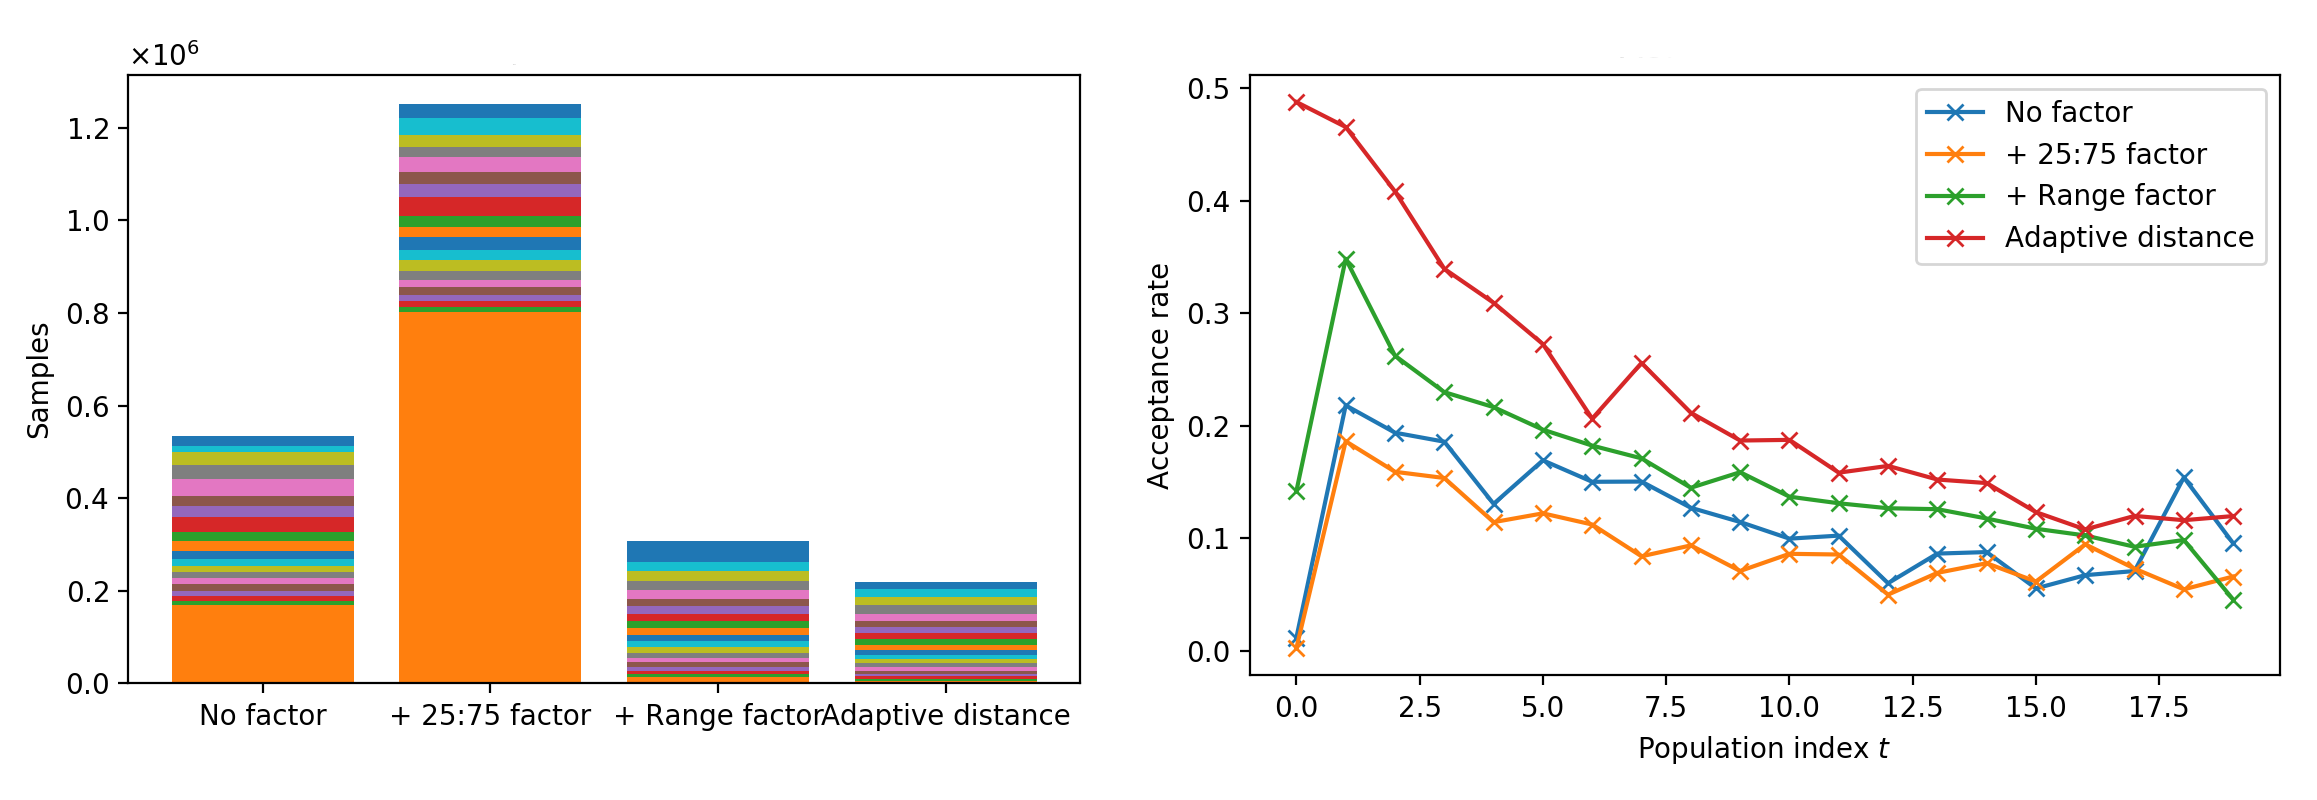
\includegraphics{fig/ib.png}}
    \end{center}

    \caption[Factors and adaptive distance experiments]%
    {Factors and adaptive distance experiments. Left: total required samples. Different color represents different generations (bottom totop: population 1 to population 20). Right: acceptance rates in each generation. }
    \label{fig:factor}

    \begin{center}
        \resizebox{1.0\hsize}{!}{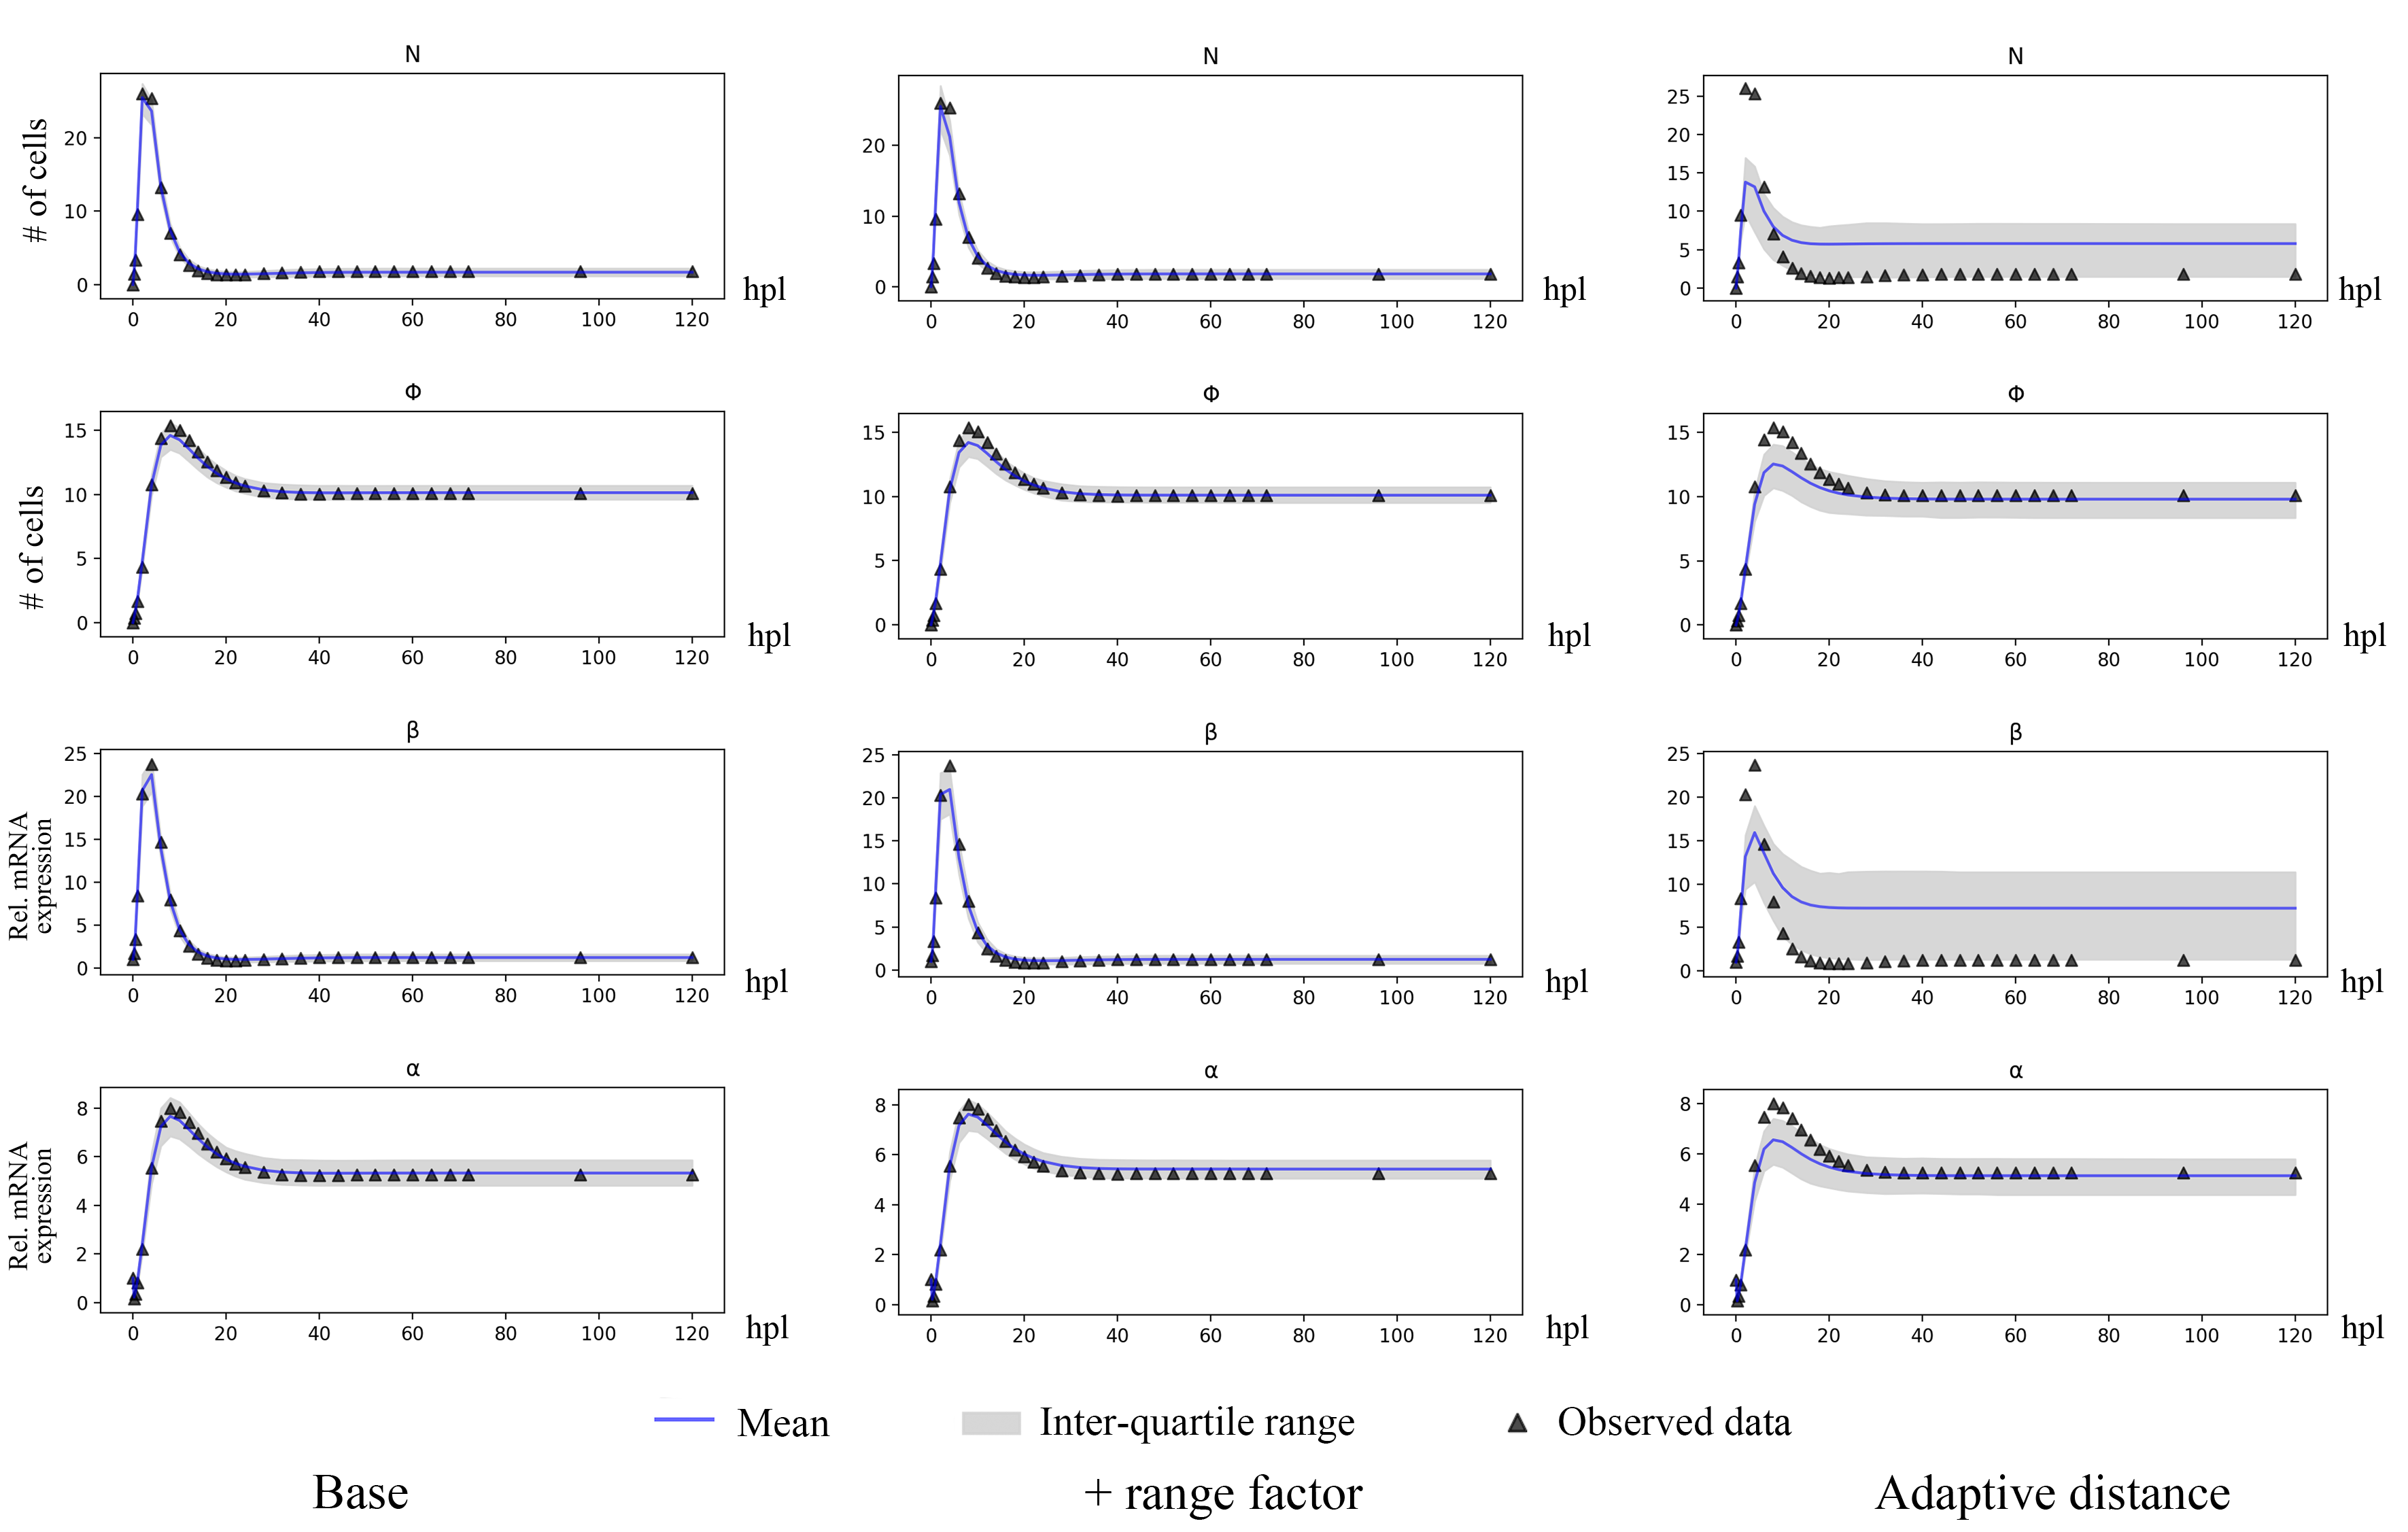
\includegraphics{fig/ib_factor.png}}
    \end{center}

    \caption[Simulated trajectories ]%
    {Simulated trajectories from the last population in the factor and adaptive distance experiment. 500 randomly chosen particles from last population are used to generate a sequence of trajectories where mean and inter-quartile range are calculated from. 25:75 factor showed very similar curve as the range factor.  
    }
    \label{fig:factor_sim}

\end{figure}

However, the result of factors adaptive distance could not be directly compared to standard run, because it changed the distance measurement by adapting weights or manually setting factors. Factors were normalise to make it more close the standard distance measurement. As a result, the same final threshold value did not guarantee that adaptive distance can reach the same level of fit as others. After 20 populations, adaptive distance had a poor fit (Figure \ref{fig:factor_sim}), while the standard run and two types of factors had similar tight fits of the data, which all converge to the true posterior. Additional in our implementations, variance factor (which tries to normalise the data according to the dependent variables' variance) was also tries and gave very similar performance as range factor.

To conclude, because the factors and weights are directly multiplied to $\Delta x$ and thus the metrics for distance are changed, the direct compare of the efficiency under the same threshold schedule was unfeasible; we could only compare the results after the same number of generations. Factors gave nearly the same inferred results but required different number of samples, hence cares must betaken when choosing factor schemes. Adaptive distance did not result in a accurate result as others. As a result, our further implementations used standard distance function, and factors were tried for possible improvements.


% by applying factors the total required samples are less, and the adaptive distance requires much less samples; their acceptance rates are also higher than the standard one. It seems that adaptive function and factors could help to converge more quickly.


% However considering the result after 20 generation (Figure \ref{fig:factor_sim}), the resultant model gives the contrary preference. Applying factors and using adaptive distance can lead the resultant model less accurate (after the same generation iterations): they have wider inter-quantile range and may requires more generations to converge. TODO

% \subsubsection{Conclusion} We noticed the significant efficiency improvement of these adaptive options; they can largely improve the acceptance rate in some cases. However, as the factors and weights are directly multiplied to $\Delta x$ and thus the metrics for distance are changed, a direct compare of the efficiency under the same threshold schedule is unfeasible; after the same number of generations they can reach a small $\epsilon_t$ but still the approximated posterior is not as accurate as the standard implementation. AS a result, our implementation of the parameter inference will only consider standard distance function and factors are only tested for improvements (FIGURE).


\subsection{Data size, prior distribution and population}

% [experiments plan]

Some other hyperparameters, e.g. feed-in data size, prior distribution, number of populations and number of particles in each population were also of our interest. Experiments were designed to explore how these options affect the goodness of fit and efficiency of the implementation.

Regarding the existing dynamic systems model, SMC was applied with two data size options, three prior distribution (uniform distribution, wider uniform distribution and log-uniform distribution). The population options i.e. population size and number of populations were also tried with different values. These experiments intended to give suggestions on the later SMC implementation on experimental data.

\subsubsection{Experiments results}

\begin{figure}[H]
    \begin{center}
        \resizebox{1.0\hsize}{!}{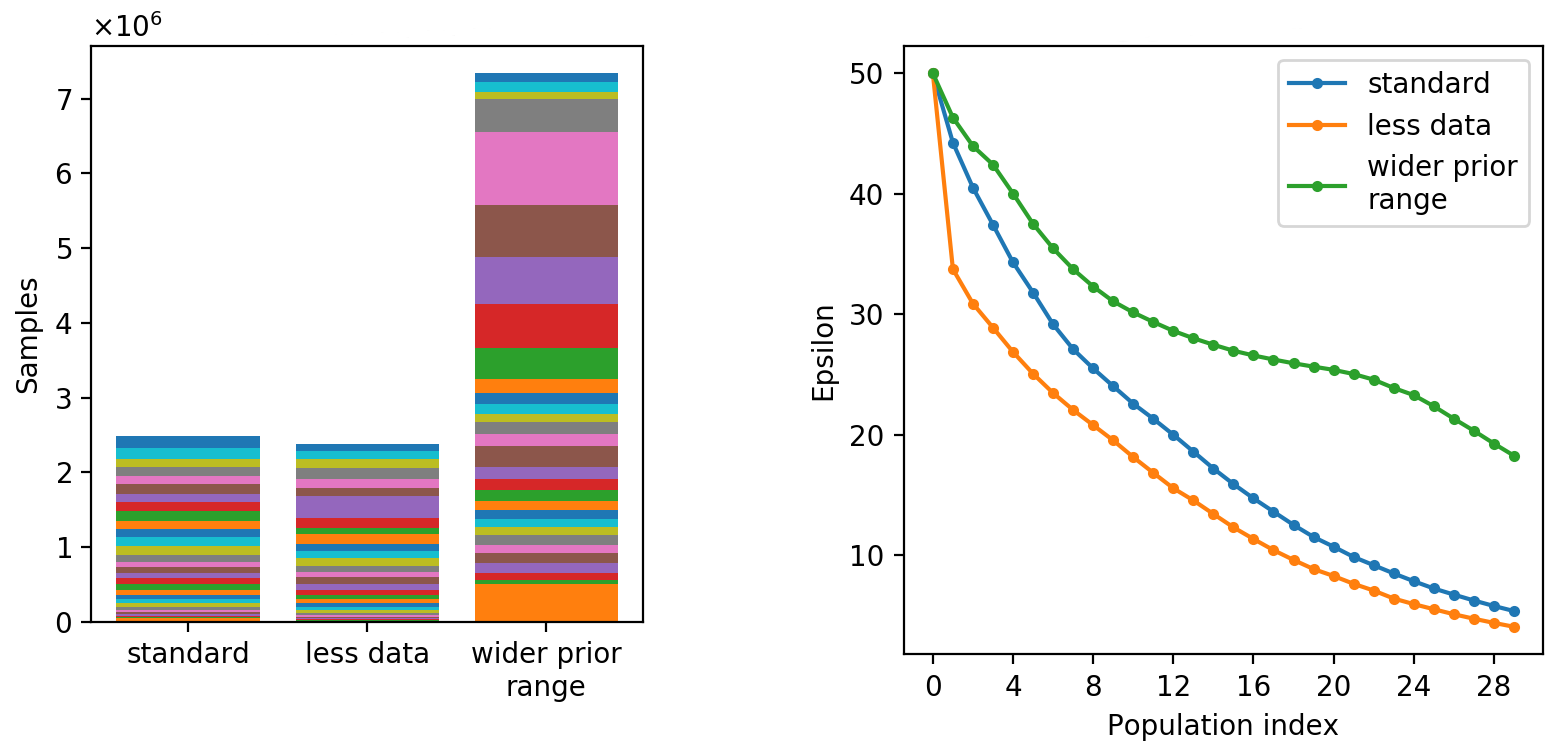
\includegraphics{fig/size1.png}}
    \end{center}

    \caption[Data size and prior distribution range experiment]%
    {Data size and prior distribution range experiment. Left: total required samples. Right: epsilon values under median epsilon schedule}
    \label{fig:size}

\end{figure}

The results from data size and prior distribution range is shown in Figure \ref{fig:size}. The standard implementation is fed with 120 data points (30 data points for each of the four variables), the `less data' is fed with 48 data points, which is the case of the real experimental measurement. Although much less (60\%) data was used, the total required sampling numbers was only 4.47\% less. This indicated that the data size does not affect the sampling process much and the inferred model are all considered acceptable when compared to the synthetic data, as they finally reached a similar epsilon threshold ((b), Figure \ref{fig:size}), but cares should still be taken when using less data point, or using other more summative statistics (e.g. mean, standard deviation, peak values, starting and ending values etc.) as the target data: as shown in \cite{ref:disease}, less data can lead to a model with more variance, under-fitting or missing some local features such as local peaks.

The prior range and distribution can largely affect the inference progress (Figure \ref{fig:size}. (a)). Samples were drawn from a high dimensional parameter space in each sampling process, a wider parameter prior interval in only one dimension can cause the parameter space to be much bigger, and consequently the exploration and sampling of parameter vectors would take much more efforts. Figure \ref{fig:size}. (b) also indicates that the convergency is slower for wider prior ranges. As a result, a proper prior interval based on our experience and belief with seeing the data should be set as narrow as possible, as inference are largely affected by the prior interval and its length; improper prior could even make the algorithm miss the true posterior \cite{ref:abcsysbio}.

How to specify prior can be tricky from problem to problem. For our task in the parameter inference of regeneration model, biologically motivated priors were used, which were general reflection of biological constrains. Also the units of the parameters help us in identify the possible scale of the parameters.


% taken from a high dimensional parameter space in each sampling process, wider prior distribution ranges will making each sampling explore more in the parameter vector space. It suggests that a narrower prior is preferred and we should make a more accurate and confident prior belief as possible for the efficiency concerns.

%     [discuss uniform and log uniform when result ready]

% [FIGURE HERE]


\subsubsection{Choise of options} 

This subsection aims to preliminarily explore options in ABC SMC implementations. From the above results, we adopted multivariate normal kernel as the kernel for our real inference on observed data; Local M-NN kernels were also planned to be tested. In the real inference, 25:75 factor were also tried to see if it could help in recovering more features and resulting a better fit. because the improvement by using less data was inapparent, we did not try to change the target summary data size. Prior intervals were explored explicitly and gradually shrunk for our models.

Some other hyperparameter, e.g. number of generations, population size (i.e. number of particles per generation) were not addressed in this subsection. In the real inference, population size was set to be greater than 2000 to avoid insufficient exploration of the previous population; in some case than high variance or uncertainties in the results were observed, population size as large as 20,000 were used. If the epsilon did not show a convergency trend, the run could be extended to more generations until a stable result was observed.

% using synthetic data with known true parameter values, thus the efficiency and the goodness of the resultant model can be compared across these options. Conclusion can be drawn to choose efficient and proper options of ABC SMC to be applied on the target models with experimental data. It also provides reference for a general inference task using SMC with high dimensional parameter space.








\section{Parameter estimation and model comparison}

\subsection{Model 1, 2 and 3}

% [separated ABC run on model 1, 2 and 3]

Using the suggested options in the previous section, the target data (Figure \ref{fig:obs_data}) is prepared as input for the SMC inference framework. Regarding the result, the population size and number of generations are adjusted several times to obtain an general informative posterior which should be stable across repeated runs and avoid local optimal as much as possible.

Parameter estimation of model 1, 2 and 3 was tried with different prior distribution setting: distribution range [0, 25] and [0, 75], amd distribution type uniform and log-uniform. All these ABC SMC runs uses 2,000 particles per population and 30 generations.

Log-uniform-shaped prior seems to give a better fit of the model, and wider prior range [0, 75] does not give a more accurate result. Then distribution range [0, 25] was tried, in case some parameter have a true posterior laying between [25, 50].

The results of prior distribution log-uniform [0, 50] is shown in Figure \ref{fig:result123}. For model 3, the acceptance rates and epsilon path are presented in Figure \ref{fig:result123_2}. For model 3, the estimated parameters' posterior is shown in Figure \ref{fig:para1}. Figure \ref{fig:result123} plots the estimated curve of models, using the mean value of each parameter's approximated posterior; also 1000 particles (each particle is a parameter set) were sampled and used to generate simulated trajectories of the four variable, and the mean (blue) and 25th to 75th percentile range (grey) are calculated from the 1000 simulated data.

Before applying model comparison methods, some features of the three model can still be compared. From simulated curves, It can be seen that all the inter-quartile ranges are tight around the mean value curve, which indicates the approximated posterior are concentrated to some degree; the peak-shaped posterior distributions (Figure \ref{fig:para1}) agrees with this. All epsilon values converges to a steady level, and model 3 has a lower final epsilon value and consequently the simulated trajectory is more close to the observed data (model 3, Figure \ref{fig:result123}).

The acceptance rates is fluctuating and have a gradually increase trend for all the three models, as the acceptance rate becomes higher when the true posteriors are gradually approximated. Compared to model 1, model 2 gives a better fit of the decreasing trend at the second half of the observed data, by using a exponentially decaying self-increase rate $\lambda_N$ instead of a constant. The resultant simulated data from model 2 and 3 are in the similar trends and the most obvious difference is that for model 3, the simulated data of $\Phi$ and $\alpha$ are more `flat'. We expect model 3 to be the best model as it reaches a threshold value and intuitively gives a better fit, although the fit could not be considered generally a good representation of the biological process that we want to model, as the simulated data are significantly biased from the observed data for tnf-$\alpha$. A sharp peak at 4 hpl is observed from the measurement (Figure \ref{fig:obs_data}) but no similar features are represented by any of the three models.

\begin{figure}
    \begin{center}
        \resizebox{1.0\hsize}{!}{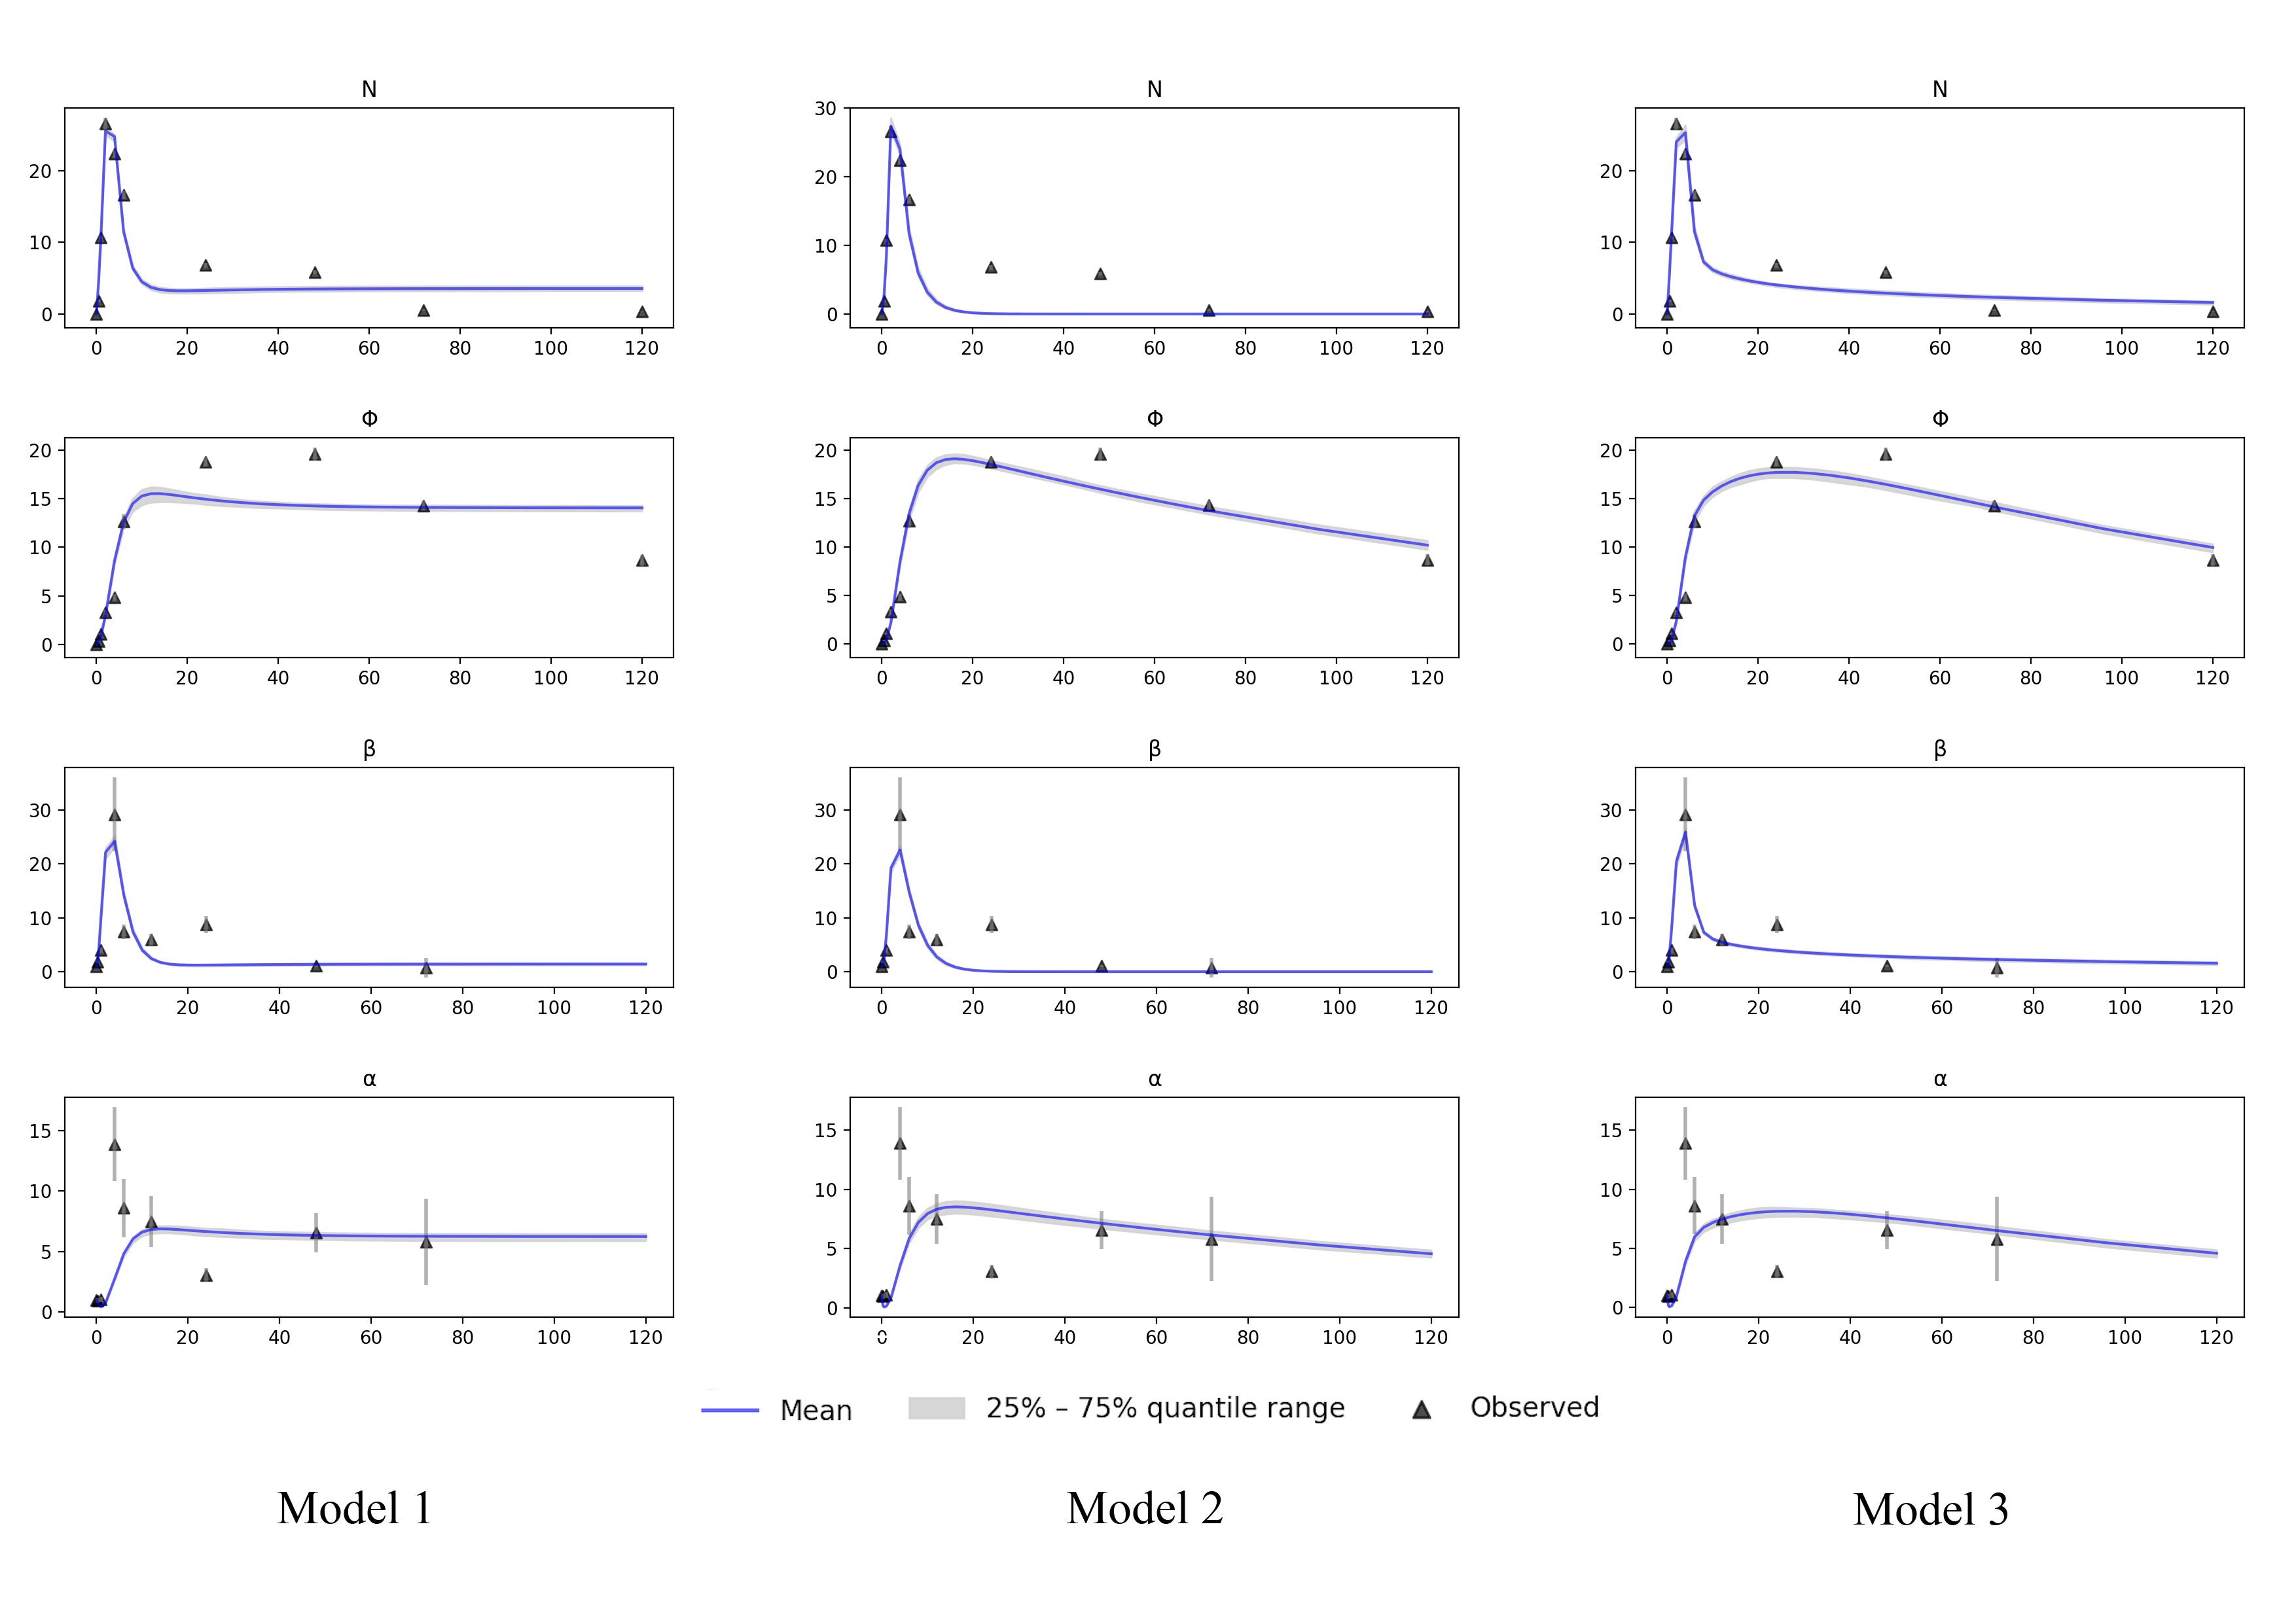
\includegraphics{fig/resultCurve123.png}}
    \end{center}

    \caption[Simulated trajectory from the 20th population of model 1, 2 and 3]%
    {Simulated trajectory from the last population of model 1, 2 and 3. Error bar indicates SEM. 500 randomly chosen particles from last population are used to generate a sequence of trajectories where mean and inter-quartile range are calculated from}
    \label{fig:result123}


    \vspace*{\floatsep}


    \begin{center}
        \resizebox{0.6\hsize}{!}{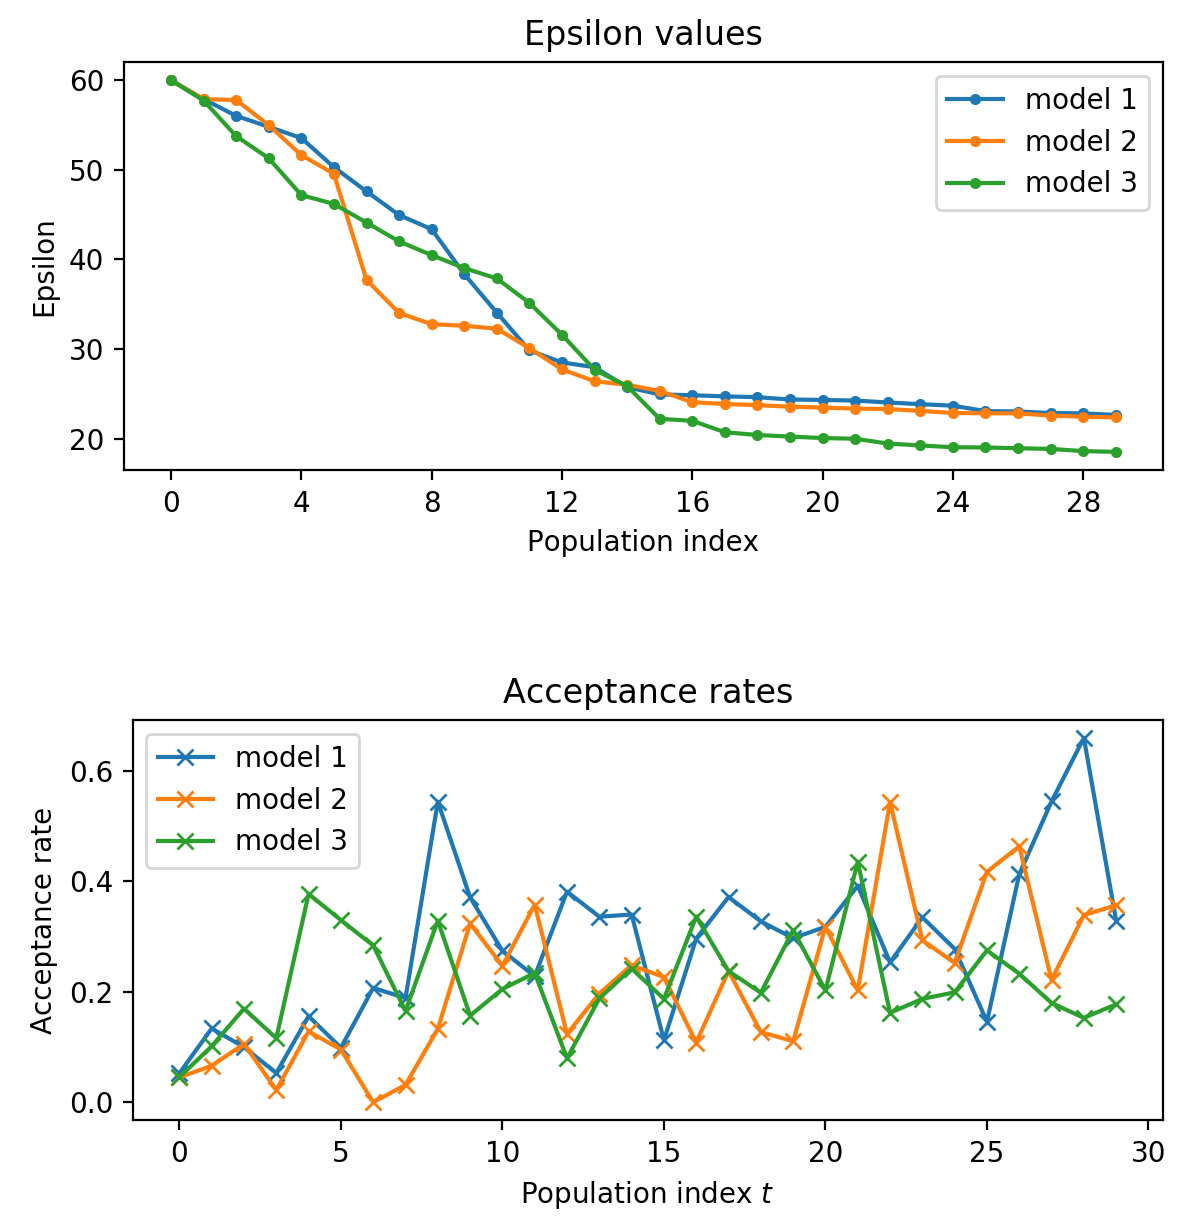
\includegraphics{fig/eps_acc123.png}}
    \end{center}

    \caption{Epsilon trends and acceptance rates of model 1, 2 and 3}
    \label{fig:result123_2}

\end{figure}

\begin{figure}
    \begin{center}
        \resizebox{1.0\hsize}{!}{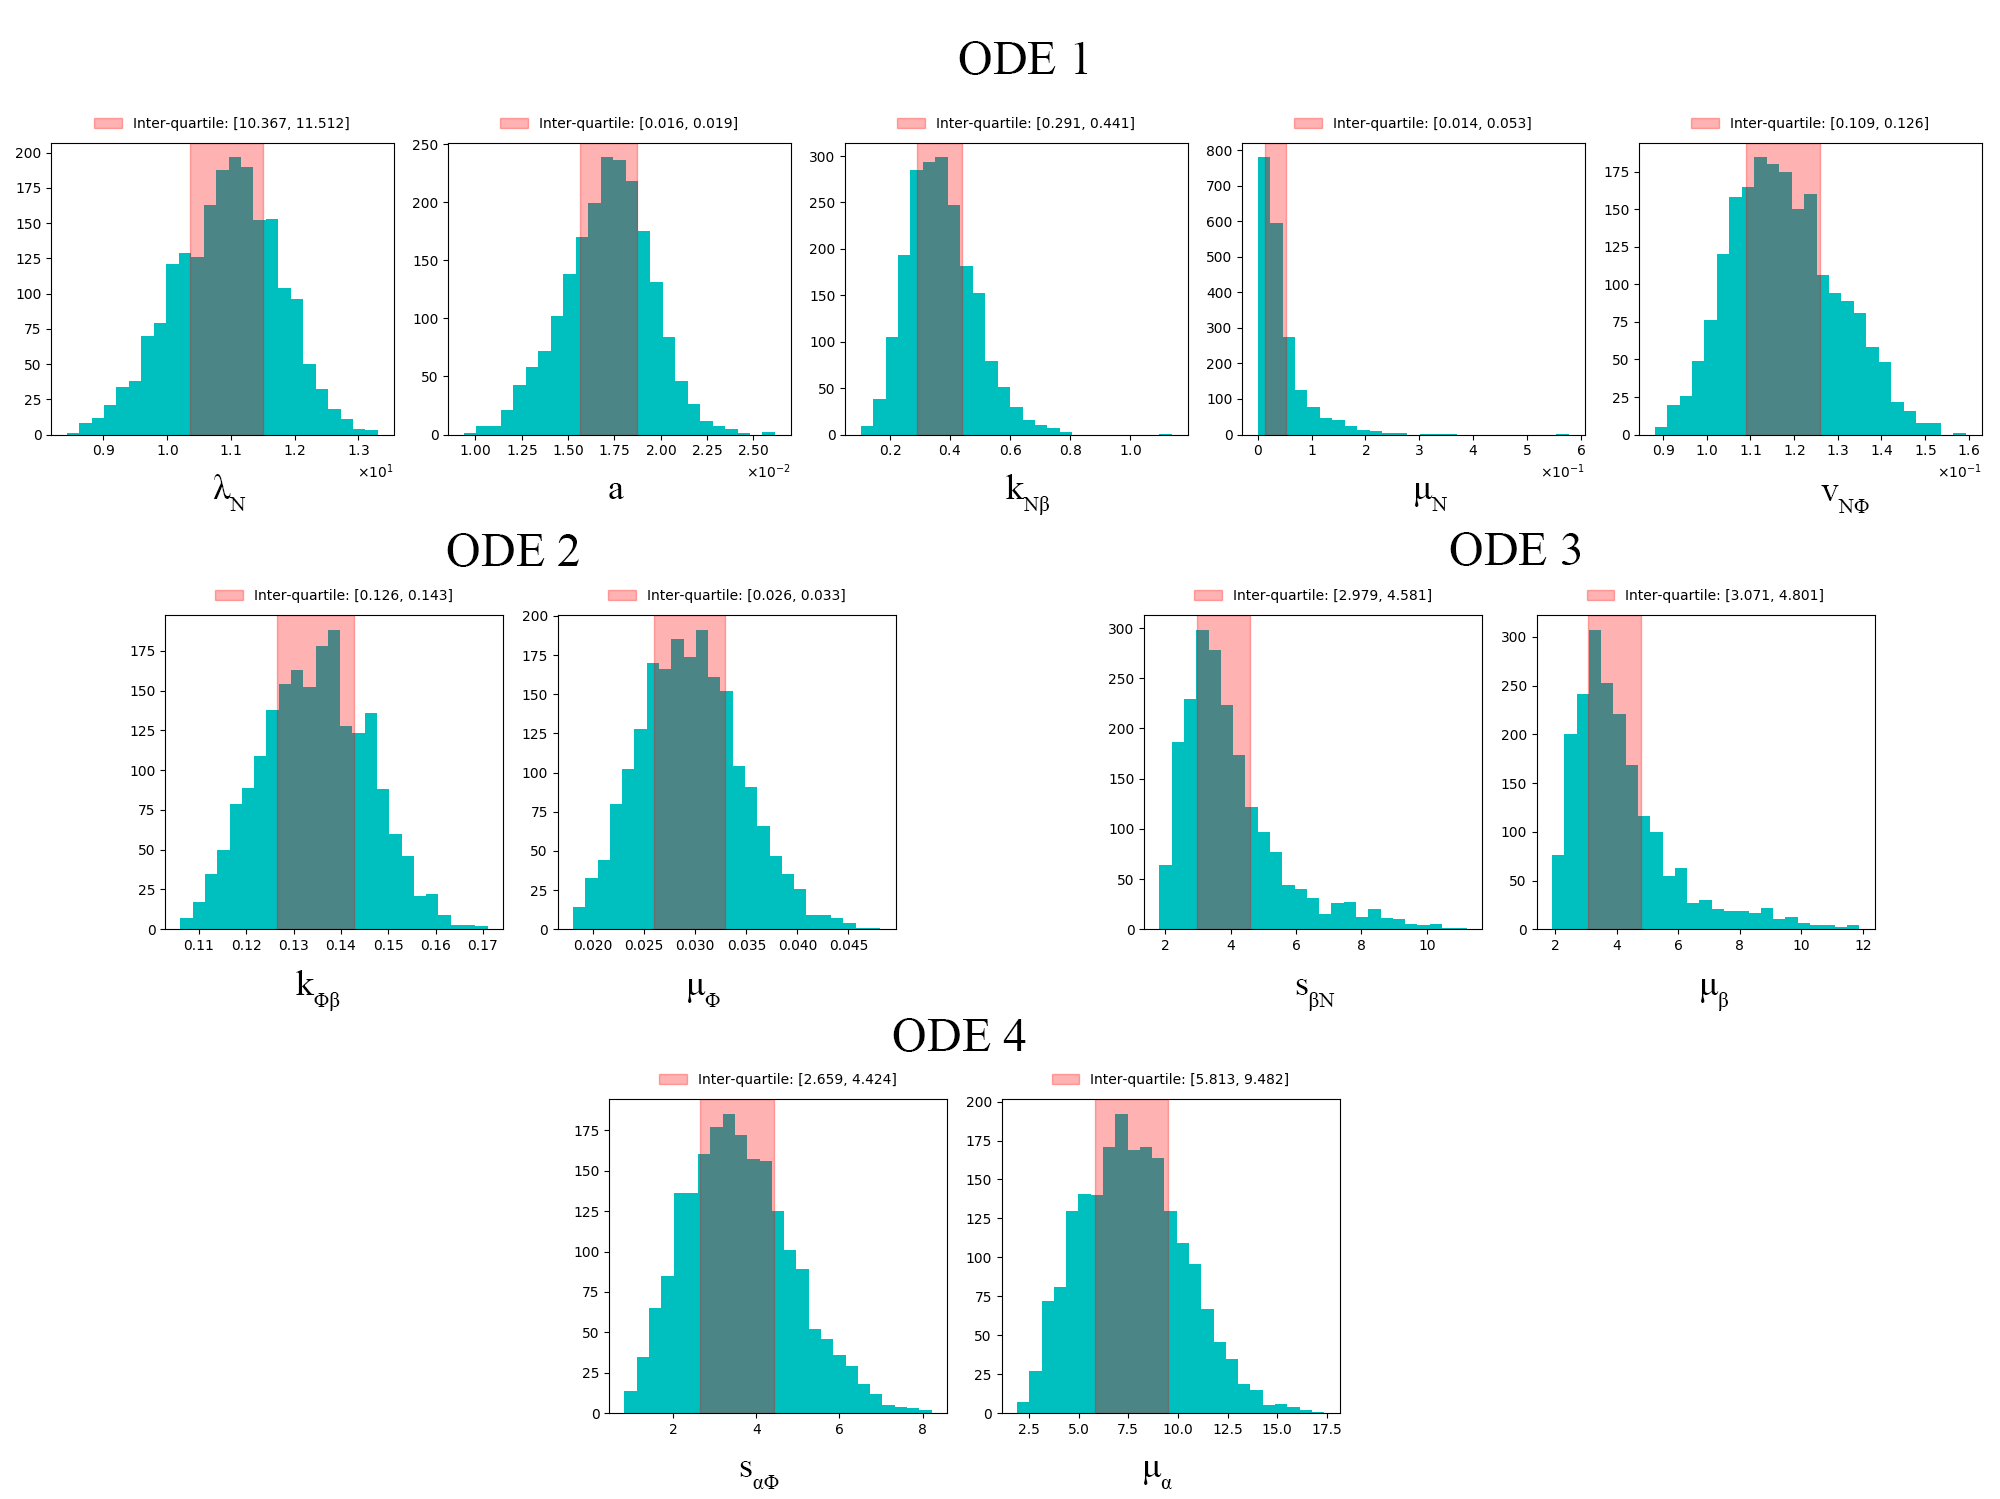
\includegraphics{fig/para1234.png}}
    \end{center}

    \caption[Estimated posterior distribution of parameters in model 3]%
    {Estimated posterior distribution of parameters in model 3. Shaded range indicates 25\%--75\% quantile of the population}
    \label{fig:para1}

    \begin{center}
        \resizebox{1.0\hsize}{!}{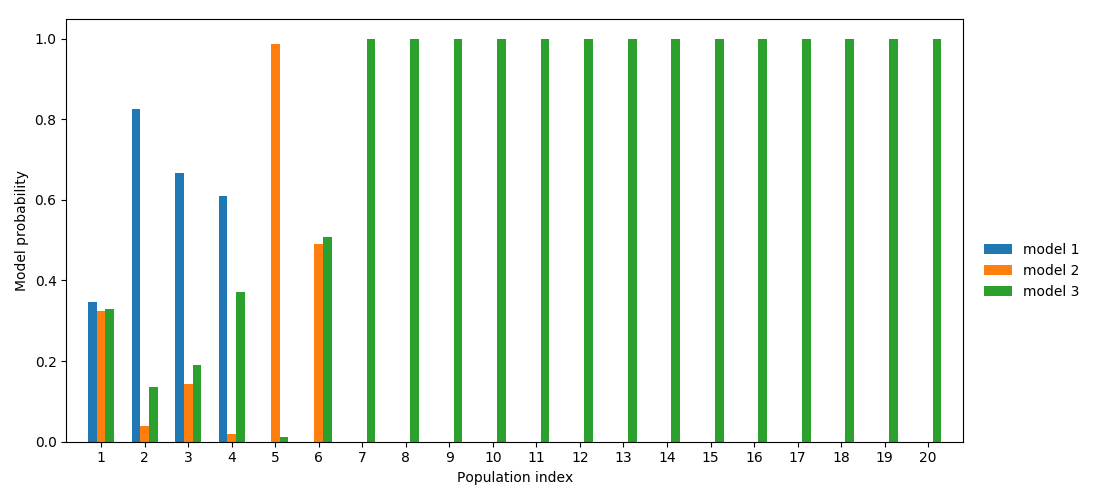
\includegraphics{fig/cmp1.png}}
    \end{center}

    \caption[ABC SMC based model comparison of model 1, 2 and 3]%
    {ABC SMC based model comparison of model 1, 2 and 3. From population 8 to population 30, model3 always wins}
    \label{fig:cmp1}

\end{figure}

[model comparison among model 1, 2, 3]

Next a model selection experiment with different prior was conducted, using the same ABC-SMC framework. As in the parameter inference, two distributions (uniform and log-uniform) are tested with three different interval ([0, 25], [0, 50] and [0, 75]). The results show that model 3 wins with nearly 100\% model probability at most runs after 30 generations, except log-uniform [0, 75]. All the model probability results are of great discrepancy (e.g. 100\% model 3 and 0\% for model 1 and 2), so Bayesian factor is not calculated.

Figure \ref{fig:cmp1} shows the model selection process, under log-uniform [0, 50] prior distribution. Model 3 gains total advantage over model 1 and 2 after 7th population. Together with conclusions above, model 3 is considered to be the the best model to represent the target data so far.



\begin{table}[t!]
    \centering
    \begin{tabular}{|c c c|}
        \hline
        Parameter            & Estimated mean  & Estimated mean      \\
                             & value (uniform) & value (log-uniform) \\[0.5ex]
        \hline\hline
        $\lambda_N$          & 14.1            & 13.3                \\
        $a$                  & 9.67            & 0.0170              \\
        $\kappa_{N\beta}$    & 18.0            & 0.259               \\
        $\mu_N$              & 13.2            & 0.0180              \\
        $\nu_{N\Phi}$        & 0.742           & 0.131               \\
        \hline
        $\kappa_{\Phi\beta}$ & 0.239           & 0.156               \\
        $\mu_\Phi$           & 0.154           & 0.0350              \\
        \hline
        $s_{\beta N}$        & 6.75            & 1.21                \\
        $\mu_\beta$          & 6.38            & 1.32                \\
        \hline
        $s_{\alpha\Phi}$     & 17.0            & 5.83                \\
        $\mu_\alpha$         & 11.9            & 2.43                \\
        \hline
    \end{tabular}
    \caption[Estimated parameter values of model 3]
    {Estimated parameter values of model 3, using uniform prior distribution and log-uniform prior distribution respectively}
    \label{table:estimated1}
\end{table}

Compared to uniform distributed prior, we found that log-uniform distributed prior is more suitable in the inference. Log-uniform results in an obviously better fit and narrower inter-quantile interval (Figure \ref{fig:result123} and \ref{fig:resultCurve_uni}), and the final epsilon value is also smaller. Log-uniform tends to assign values that are close to the left boundary (i.e. zero in our case) higher density, i.e. they are more likely to be sampled in the first population. As a result, the estimated parameter posteriors are expected to have smaller mean and/or skewed to left of the x-axis. The estimated values proved this (see \ref{table:estimated1}; also observed in other models and prior interval experiments). It indicates that some of the true parameter tend to have small values that are close to zero, and using log-uniform distribution could results in a faster and more satisfying inference. Regarding this, further experiments all use log-uniform distribution only.


\subsection{Model 4 and 5}

[features that derive model 4 and 5]

We observed that the existing models cannot well represent the trajectory of relative expression of tnf-$\alpha$: from experimental data, a rapid increase of tnf-$\alpha$ expression is observed in 0--4 hpl, followed by a rapid drop; all the models cannot well recover this feature and most test results see a less-rapid increase followed by a gradually decree and the observed peak value is not reached (e.g. Figure \ref{fig:result123}). Also in some other case e.g. Figure \ref{fig:resultCurve_uni}, tnf-$\alpha$ trajectories is well fitted at the cost of under-fitting $\Phi$. Hence efforts had been spent to propose more alternative models that can possibly solve this problem.

The two proposed alternative models is based on model 3 and try to add extra term in the tnf-$\alpha$ equation $\mathrm{d} \alpha/\mathrm{d} t$. As macrophage is the main source of tnf-$\alpha$ production, and a similar sharp increase-and-drop trend is observed in the il-1$\beta$ trajectory, two hypothesis and corresponding terms are propose as follows.

\paragraph{Model 4} It is assumed that the expression of il-1$\beta$ would have a promoting effect, representing by a phenomenological term $d_{\beta\alpha}\beta$ and $d_{\beta\alpha}$ is a new model parameter (positive constant). The promoting effect here is regarded to have the equivalent effect as directly promoting by il-1$\beta$, but the underlying mechanism is unclear so far. In mathematical view, this additional term can accelerate the expression of tnf-$\alpha$ in the first few time points and help to recover the peak-shaped trajectory. The proposed model is written as Equation \ref{eq:model4}.

\paragraph{Model 5} Alternatively, we considered promotions to the tnf-$\alpha$ production, i.e. $s_{\alpha\Phi}\Phi$. It is assumed that il-$\beta$ could accelerate the production process. An additional term $f_{\beta\alpha}\beta$ is introduced to production rate, with $f_{\beta\alpha}$ being a new model parameter (positive constant). This model meets the biological context considering the source of tnf-$\alpha$. The proposed model is written as Equation \ref{eq:model5}.

[further comparison of model 3, 4 and 5]

Model 4 and 5 are base on model 3, so in this phase experiments of these three models are conducted for separately parameter inference and overall model comparison. Based on our experience in conducted experiments, we used the following setting for parameter inference:

\begin{itemize}
    \item population size: 2000 and 5000
    \item number of populations: 30 generations
    \item prior: [0, 50] log-uniform
    \item perturbation kernel: multivariate normal kernel
\end{itemize}

Factors (Equation \ref{dis_f}) are also tried to find if we can force the inference framework to give more importance on the first few data points. In this experiment, for each trajectory first 8 data points are assigned higher factors (0.75), and the rest 4 data points are assigned with lower factors (0.25). All these runs are conducted on remote machines and the output database files are retrieved form analysis.

Figure \ref{fig:resultCurve345} shows the simulated data from the inferred models, with population size 2000. It can be seen that the addressed problem in the trajectory of tnf-$\alpha$ is partially relieved in model 4 and 5: compared to model 3, a peak appears around 4 hpl; it can represent more features in the observed data and consequently the final reached epsilon (after 30 populations) is smaller than that of model 3, which proves that our proposed modifications in model 4 and 5 are helpful in recovering more features in observed data.

\begin{figure}
    \begin{center}
        \resizebox{1.0\hsize}{!}{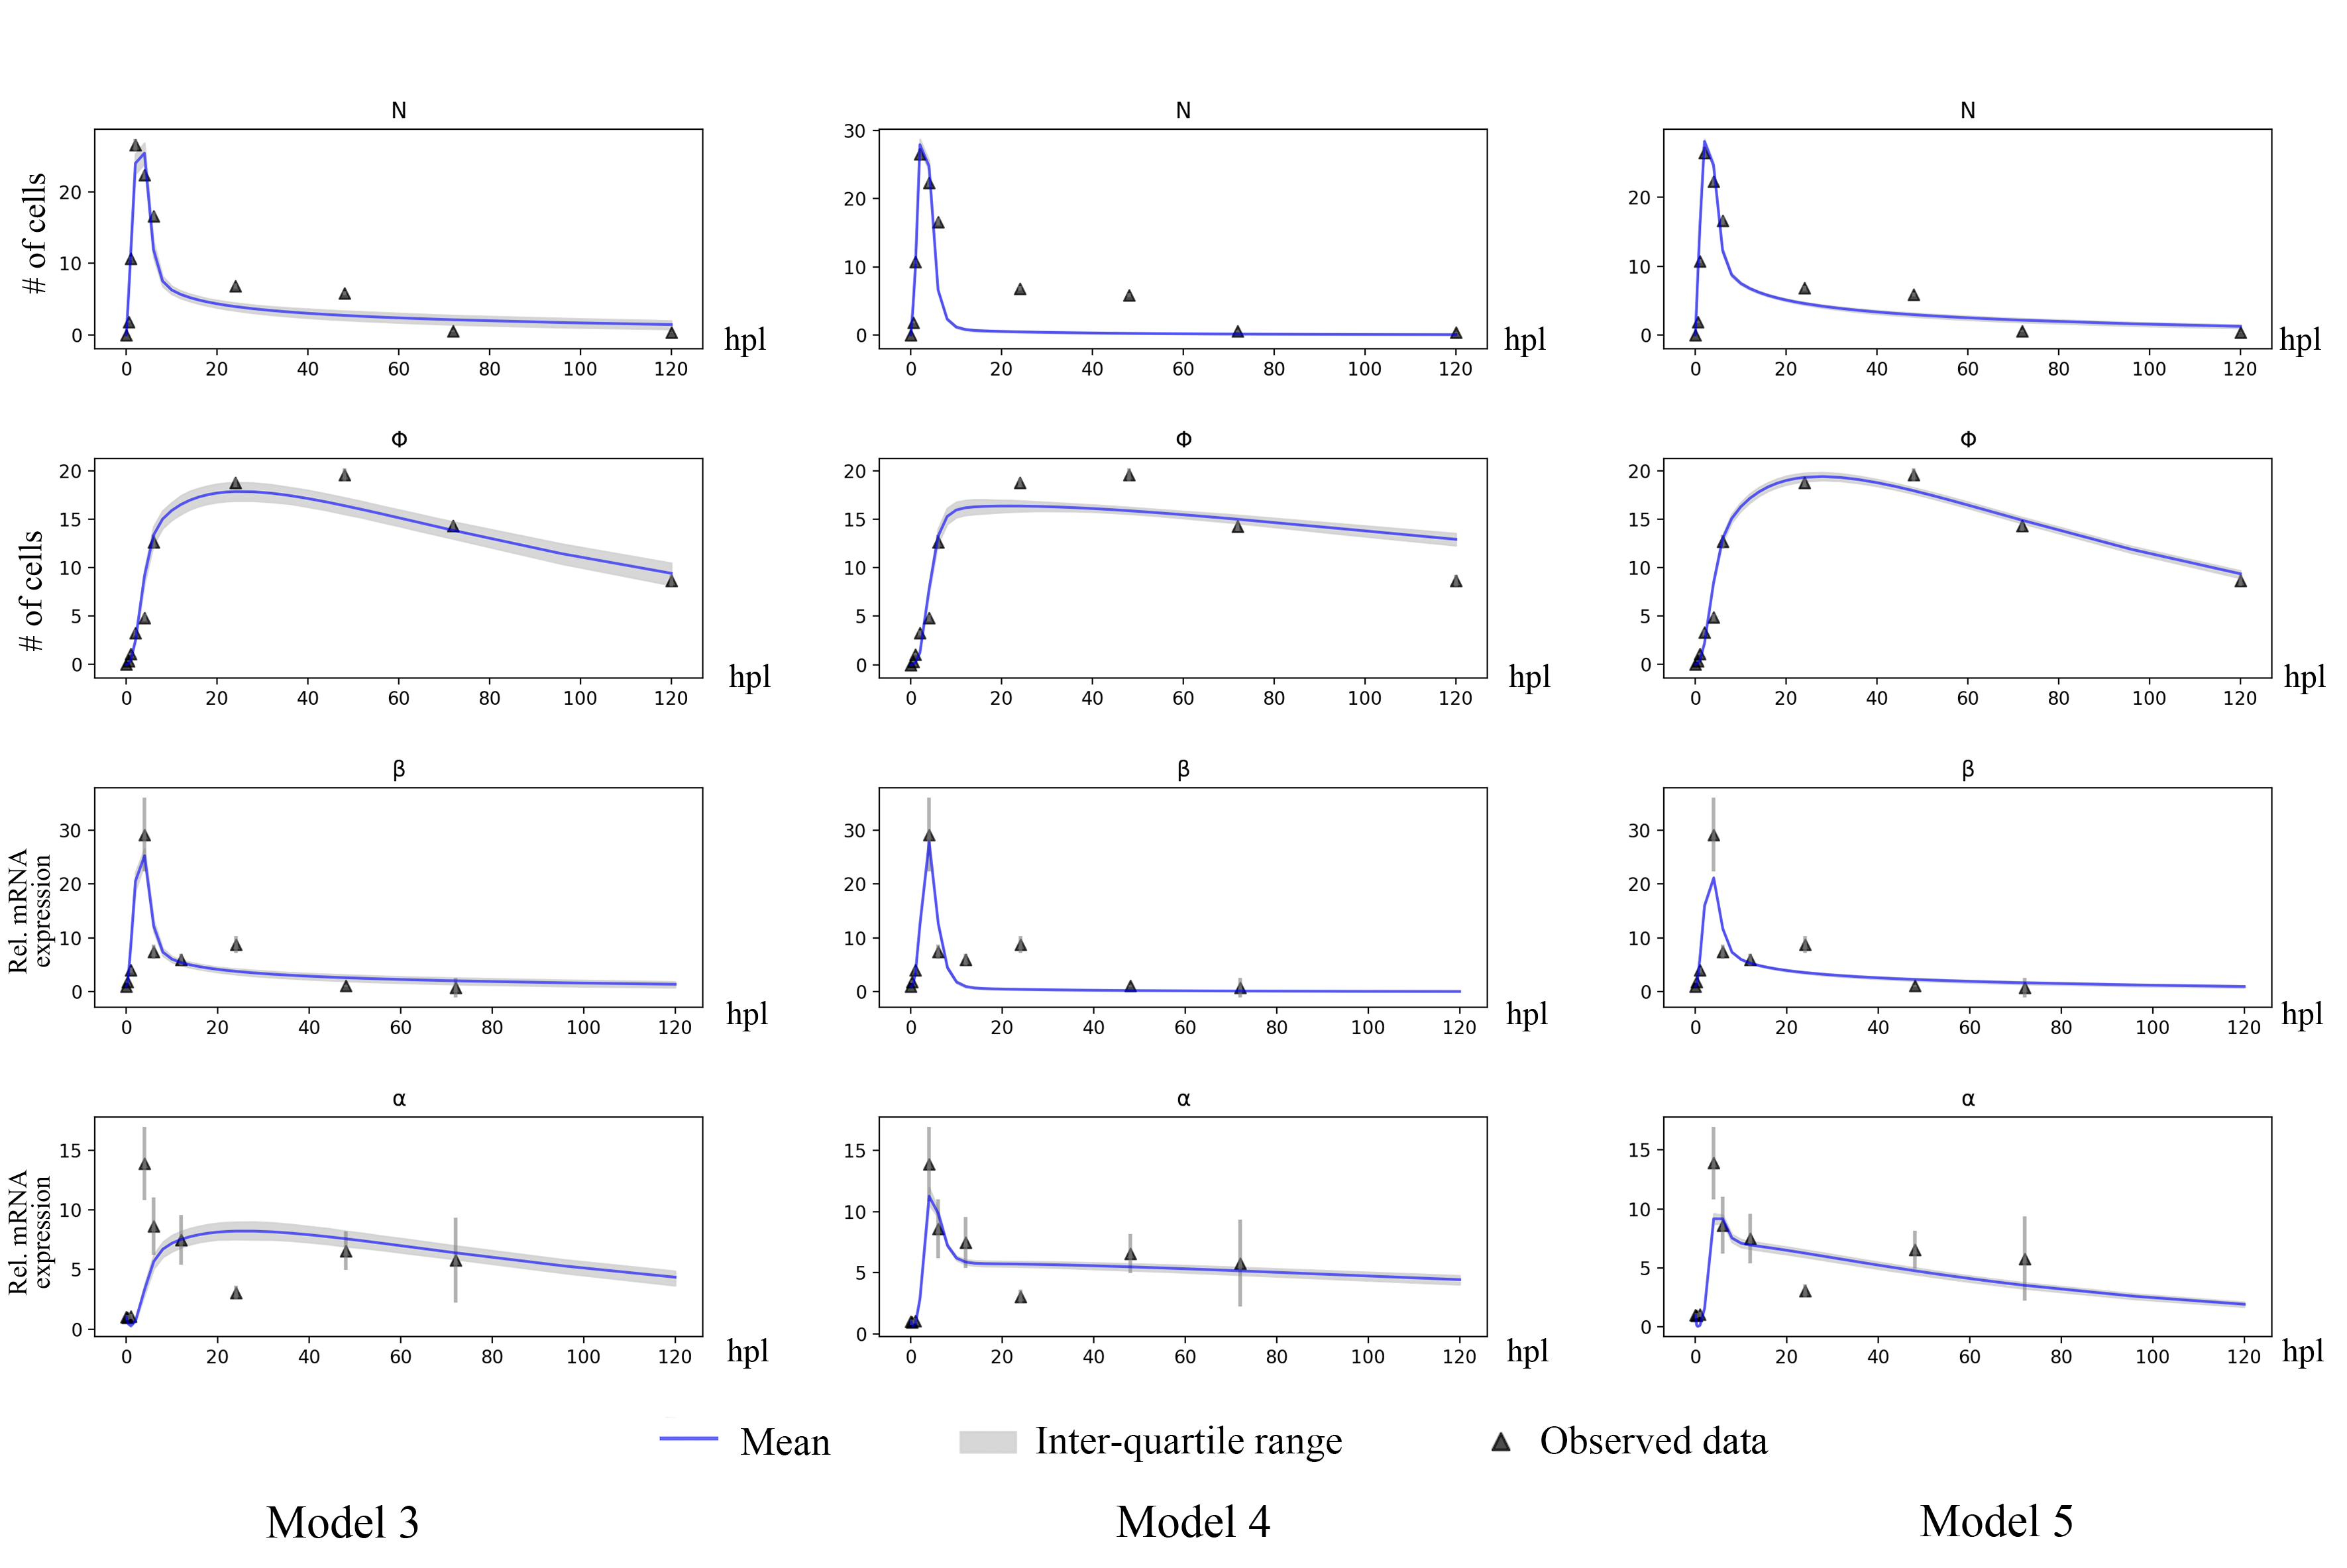
\includegraphics{fig/resultCurve345.png}}
    \end{center}

    \caption{Simulated data from the last population of model 3, 4 and 5. Error bar indicates SEM (for $N$ and $\Phi$ the SEM is relatively small)}
    \label{fig:resultCurve345}

\end{figure}

By intuition model 4 and 5 would be the best models sofar that can recover most of observed data features. Model 1, 2 and 3 con also converge to a low final epsilon value (~20), but a key feature observed in target data -- a peak at around 4 hpl -- is not fitted. Some features, e.g. fluctuations in il-1$\beta$ and tnf-$alpha$ trajectories at around 20 hpl are still not ideally fitted; all existing models give a steady or gradually decrease trends for all the four variables after 20 hpl, and fluctuations in the observed data are fitted by smooth and steady curves.

After applying factors, the results were not largely different. As expected, applying factors made the data points at first half (where exists most of the fluctuations) more `focused', however the inferred models are close to one without factors, which could indicate that for model 4 and 5, applying factors will not largely affect the final convergency and the resultant posterior.

When we are trying more generations with factors, an `over-fitting' behaviour was observed at the trajectory of macrophage (Figure \ref{fig:overfit}). In this case, the discrepancy of simulated data and observed data mainly comes from the last 2 data point (72 hpl and 120 hpl) of macrophage. As additional importance was assigned the the first few data points of each trajectory, the inference algorithm tended to preferentially fit first data points and thus relative large discrepancy at the tails were acceptable.

\begin{figure}[H]
    \begin{center}
        \resizebox{1.0\hsize}{!}{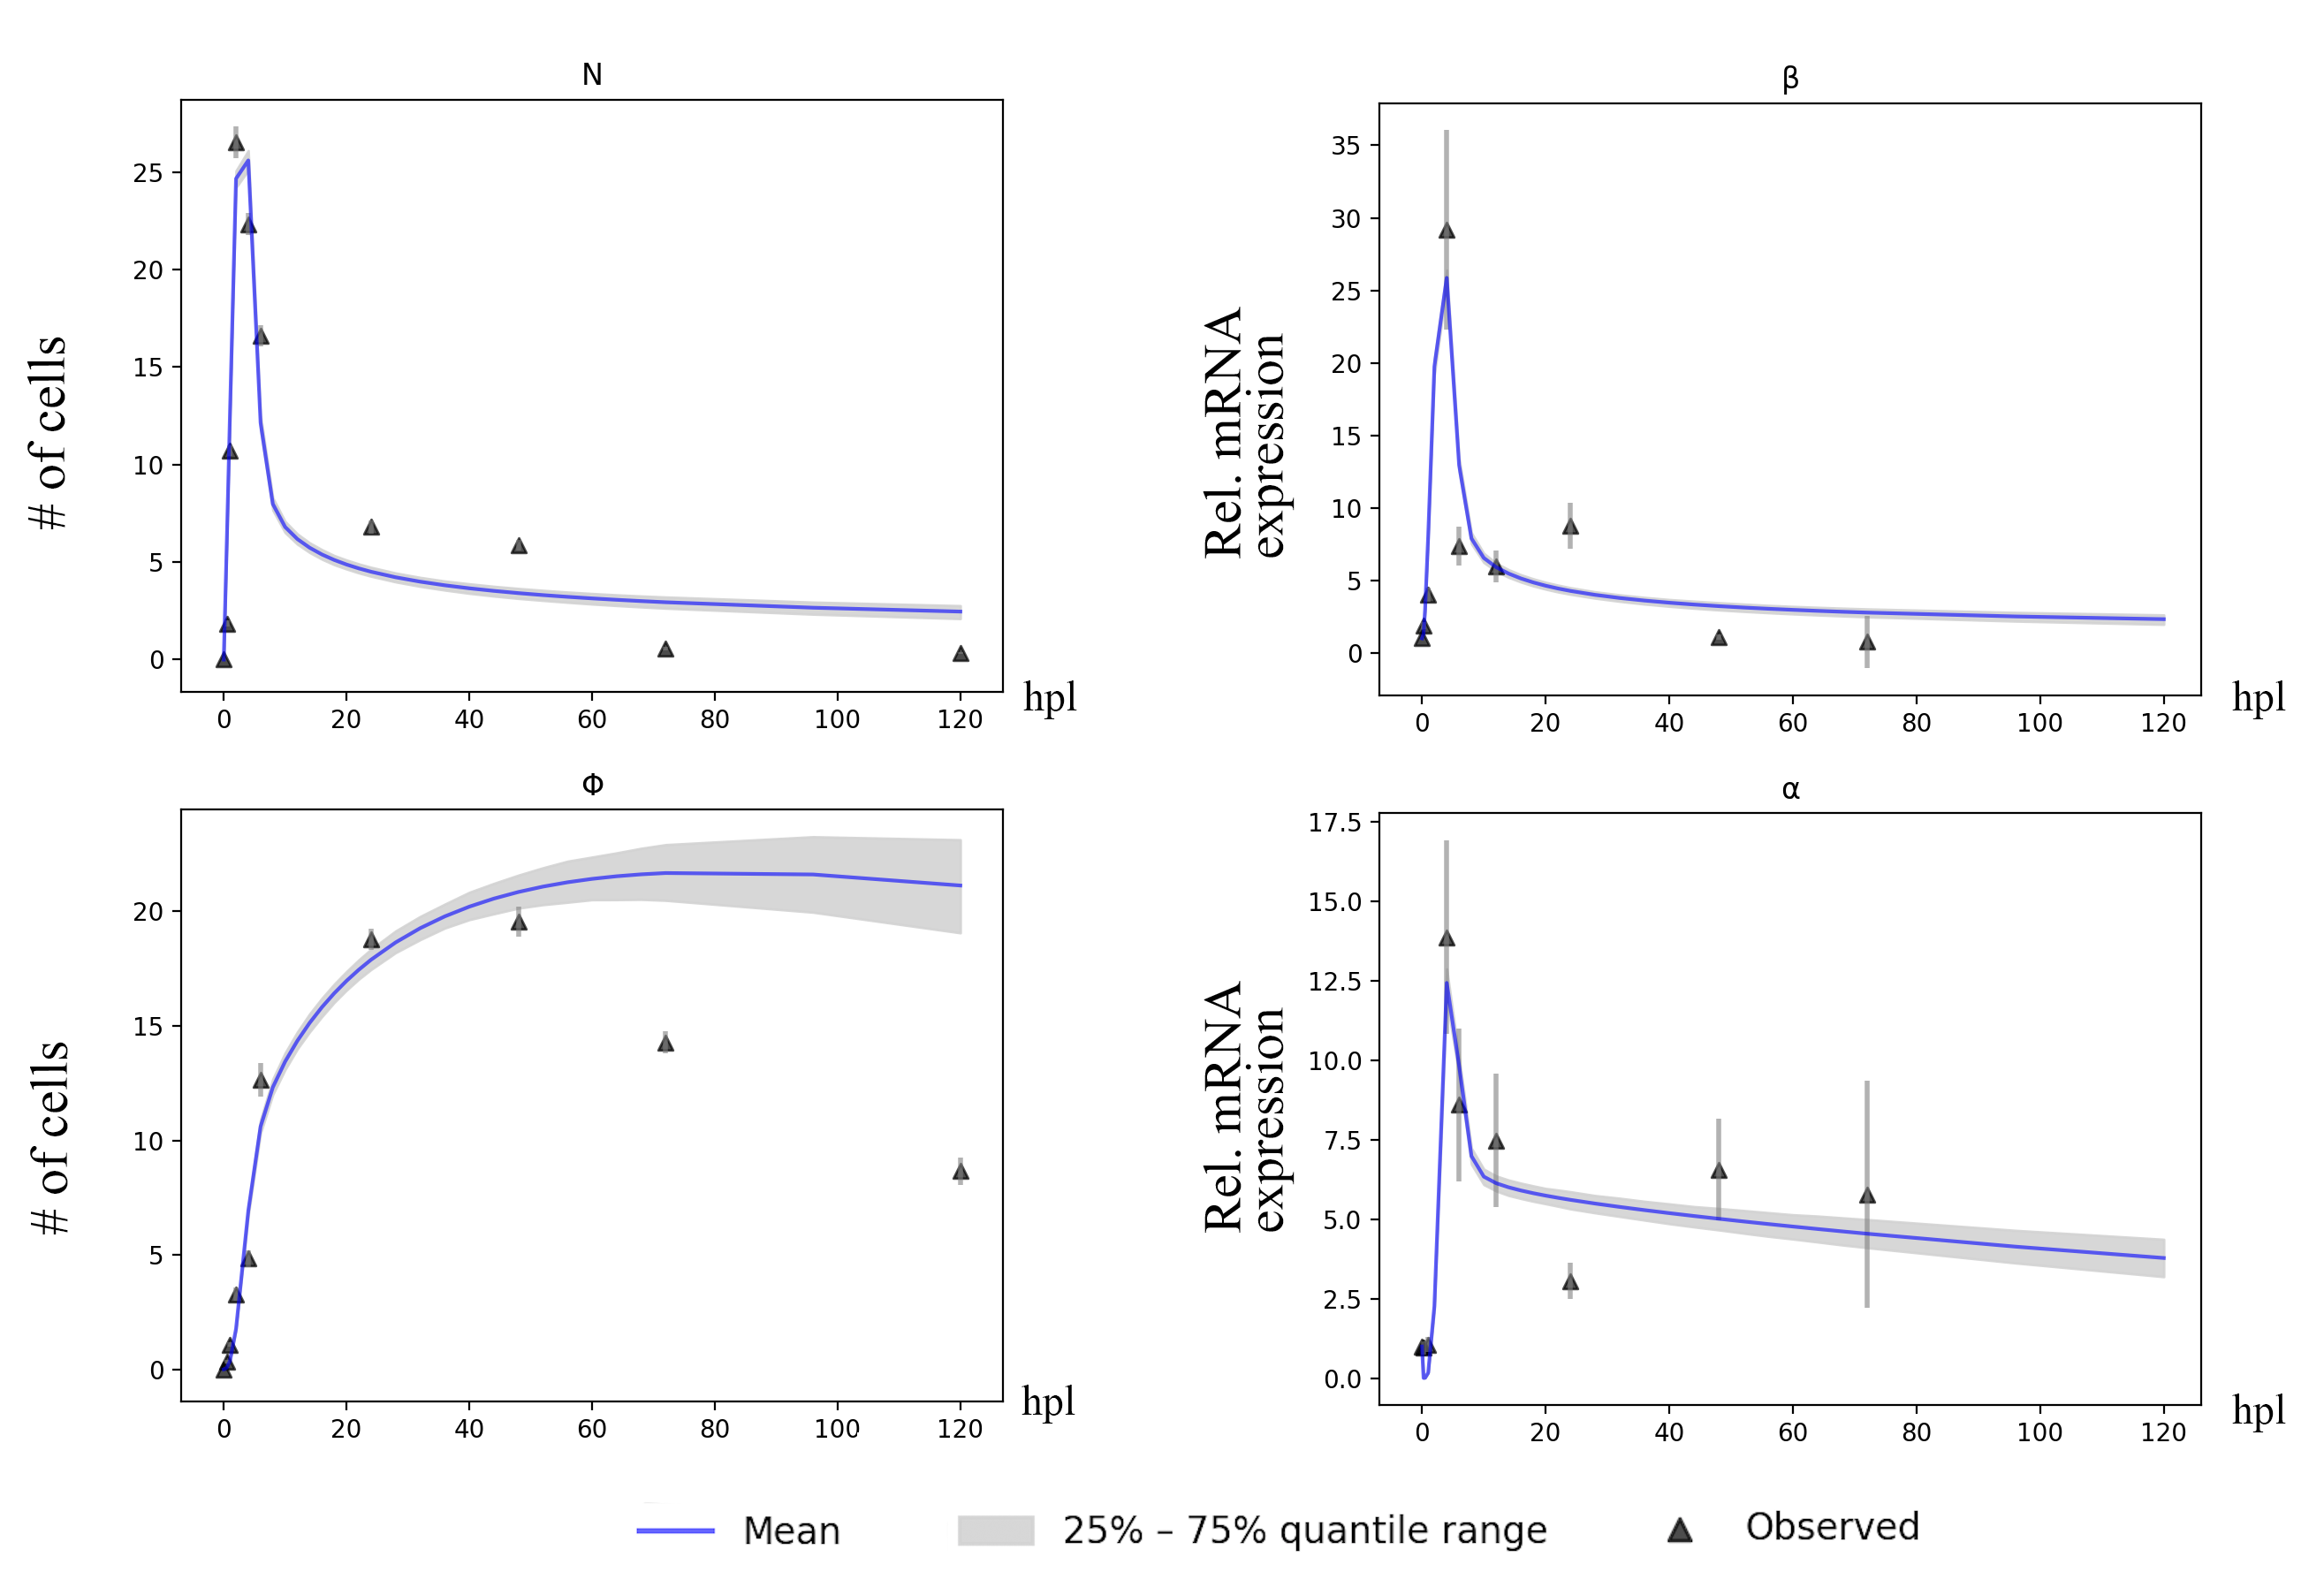
\includegraphics{fig/overfit.png}}
    \end{center}

    \caption[Simulated trajectory from the 30th population of model 5, with 25:75 factor applied]{Simulated trajectory from the 30th population of model 5, with 25:75 factor applied. Error bar indicates SEM (for $N$ and $\Phi$ the SEM is relatively small).}
    \label{fig:overfit}
\end{figure}


Next, we performed a model comparison on model 3, 4 and 5, using the same ABC SMC inference framework. Figure \ref{fig:model345cmp} shows the model probabilities at different generations.

\begin{figure}[H]
    \begin{center}
        \resizebox{1.0\hsize}{!}{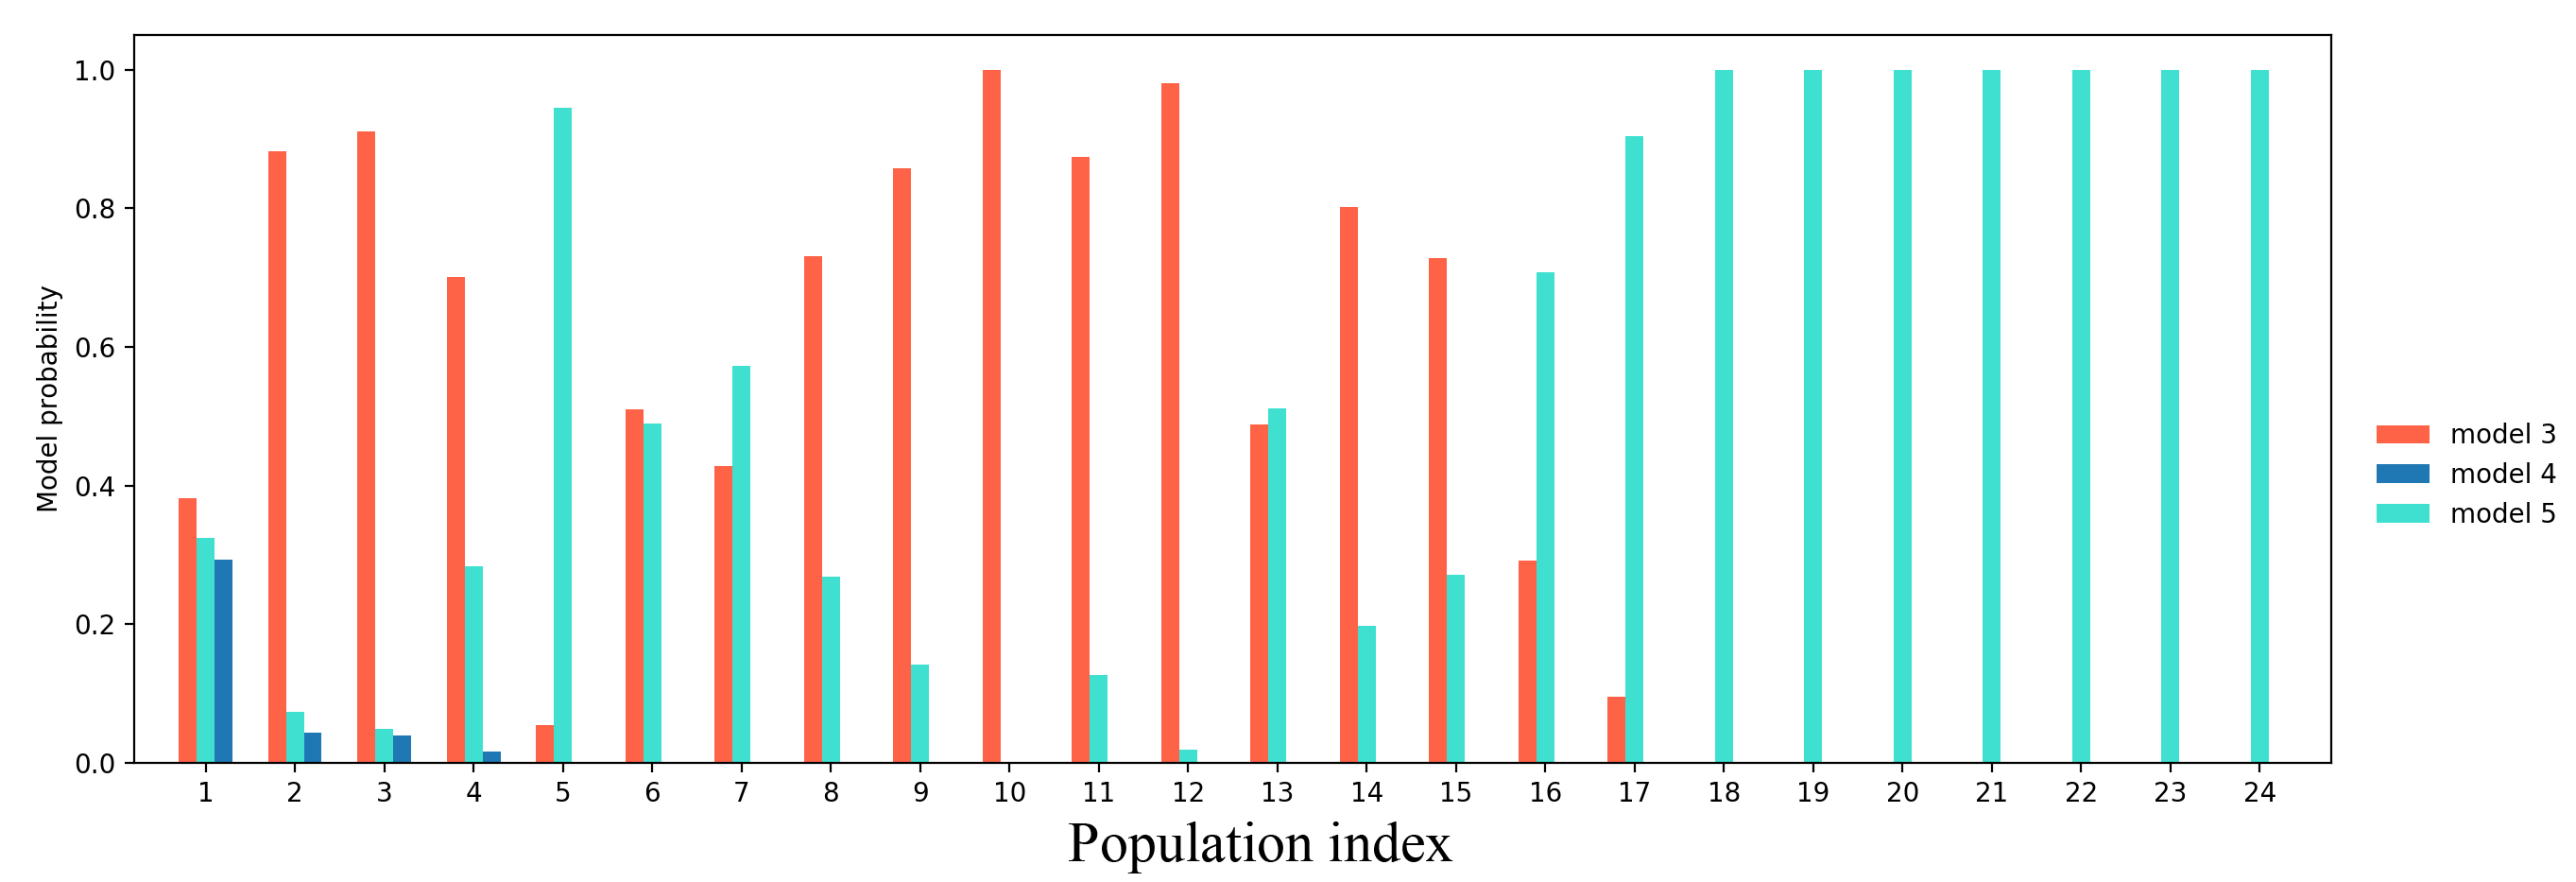
\includegraphics{fig/model345cmp.png}}
    \end{center}

    \caption[Model probabilities of model 3, 4 and 5 in ABC SMC based model comparison]{Model probabilities of model 3, 4 and 5 in ABC SMC based model comparison. Model 5 also wins in further populations (population 25 to 30)}
    \label{fig:model345cmp}
\end{figure}

Model 4 did not overweight other models across all the generations; model 3 gained advantage before generation 15 except generation 5. After generation 18 ($\epsilon_{18} = 16.98$), model 5 gained absolute advantage and won in further generations. Also, repeated runs showed similar trends: although uncertainties were present before generation 20, model 5 won with nearly 100\% probability in later generations where epsilon values were considerably low, i.e. $\epsilon_t<16$.

Based on the model comparison results, we could conclude that model 5 was the best model among the tested models. Uncertainties were observed in early generations, where similar patterns were also observed in the model comparison of model 1, 2 and 3. We considered the the violently changing model probability in early generations is related to the inference ability at high epsilon threshold values (epsilon) and possibly the insufficient exploration of the parameter space. However as we only focused on the best model with small final threshold $\epsilon_T$, the easiest way is to extended the number of generation until epsilon converges, or increase the population size for a more statistically confident probability.


% From population 10 to population 20 model 4 gains advantage but after population 20 model 5 is preferred. Again, as DISCUSSED in the model comparison of model 1, 2 and 3, Given the present result, model 5 is regarded as the best model. 

% Some further experiments tried larger population size (10,000 particles per population) and more populations (36 populations), but the resultant model did not have a significantly better fit of the observed data, although much more computation resources are used. 

For the best model (model 5), the inferred parameter posterior distribution of model 5 is shown in Figure \ref{fig:model5_para}, the estimated mean values is shown in Table \ref{table:estimated5}. The pair-wise joint density distribution is shown in Figure \ref{fig:model5_para_joint}. Most of inferred posteriors show a bell-shaped density distribution, indicating that they are gaussian distributed. A thin and concentrated shape indicate a well inferred parameter, e.g. $\mu{\Phi}$ and $\kappa_{\Phi\beta}$. Some distributions, however, are skewed to zero, e.g. $\mu_N$ ans $s_{\alpha\Phi}$.

By looking at the joint density plot (Figure \ref{fig:model5_para_joint}), some correlated patterns are observed. For example, an obvious linear relationship on the distributions of $\mu_\beta$ and $s_{\beta\Phi}$. This leads us to consider that reducing the number of parameters in the model is possible. Highly correlated parameters can be reduced, e.g. $s_{\beta\Phi}$ can be expressed as $A\mu_\beta+B$ where $A$ and $B$ can be calculated from the joint distribution by fitting a linear regression.

\begin{figure}[ht]
    \begin{center}
        \resizebox{1.0\hsize}{!}{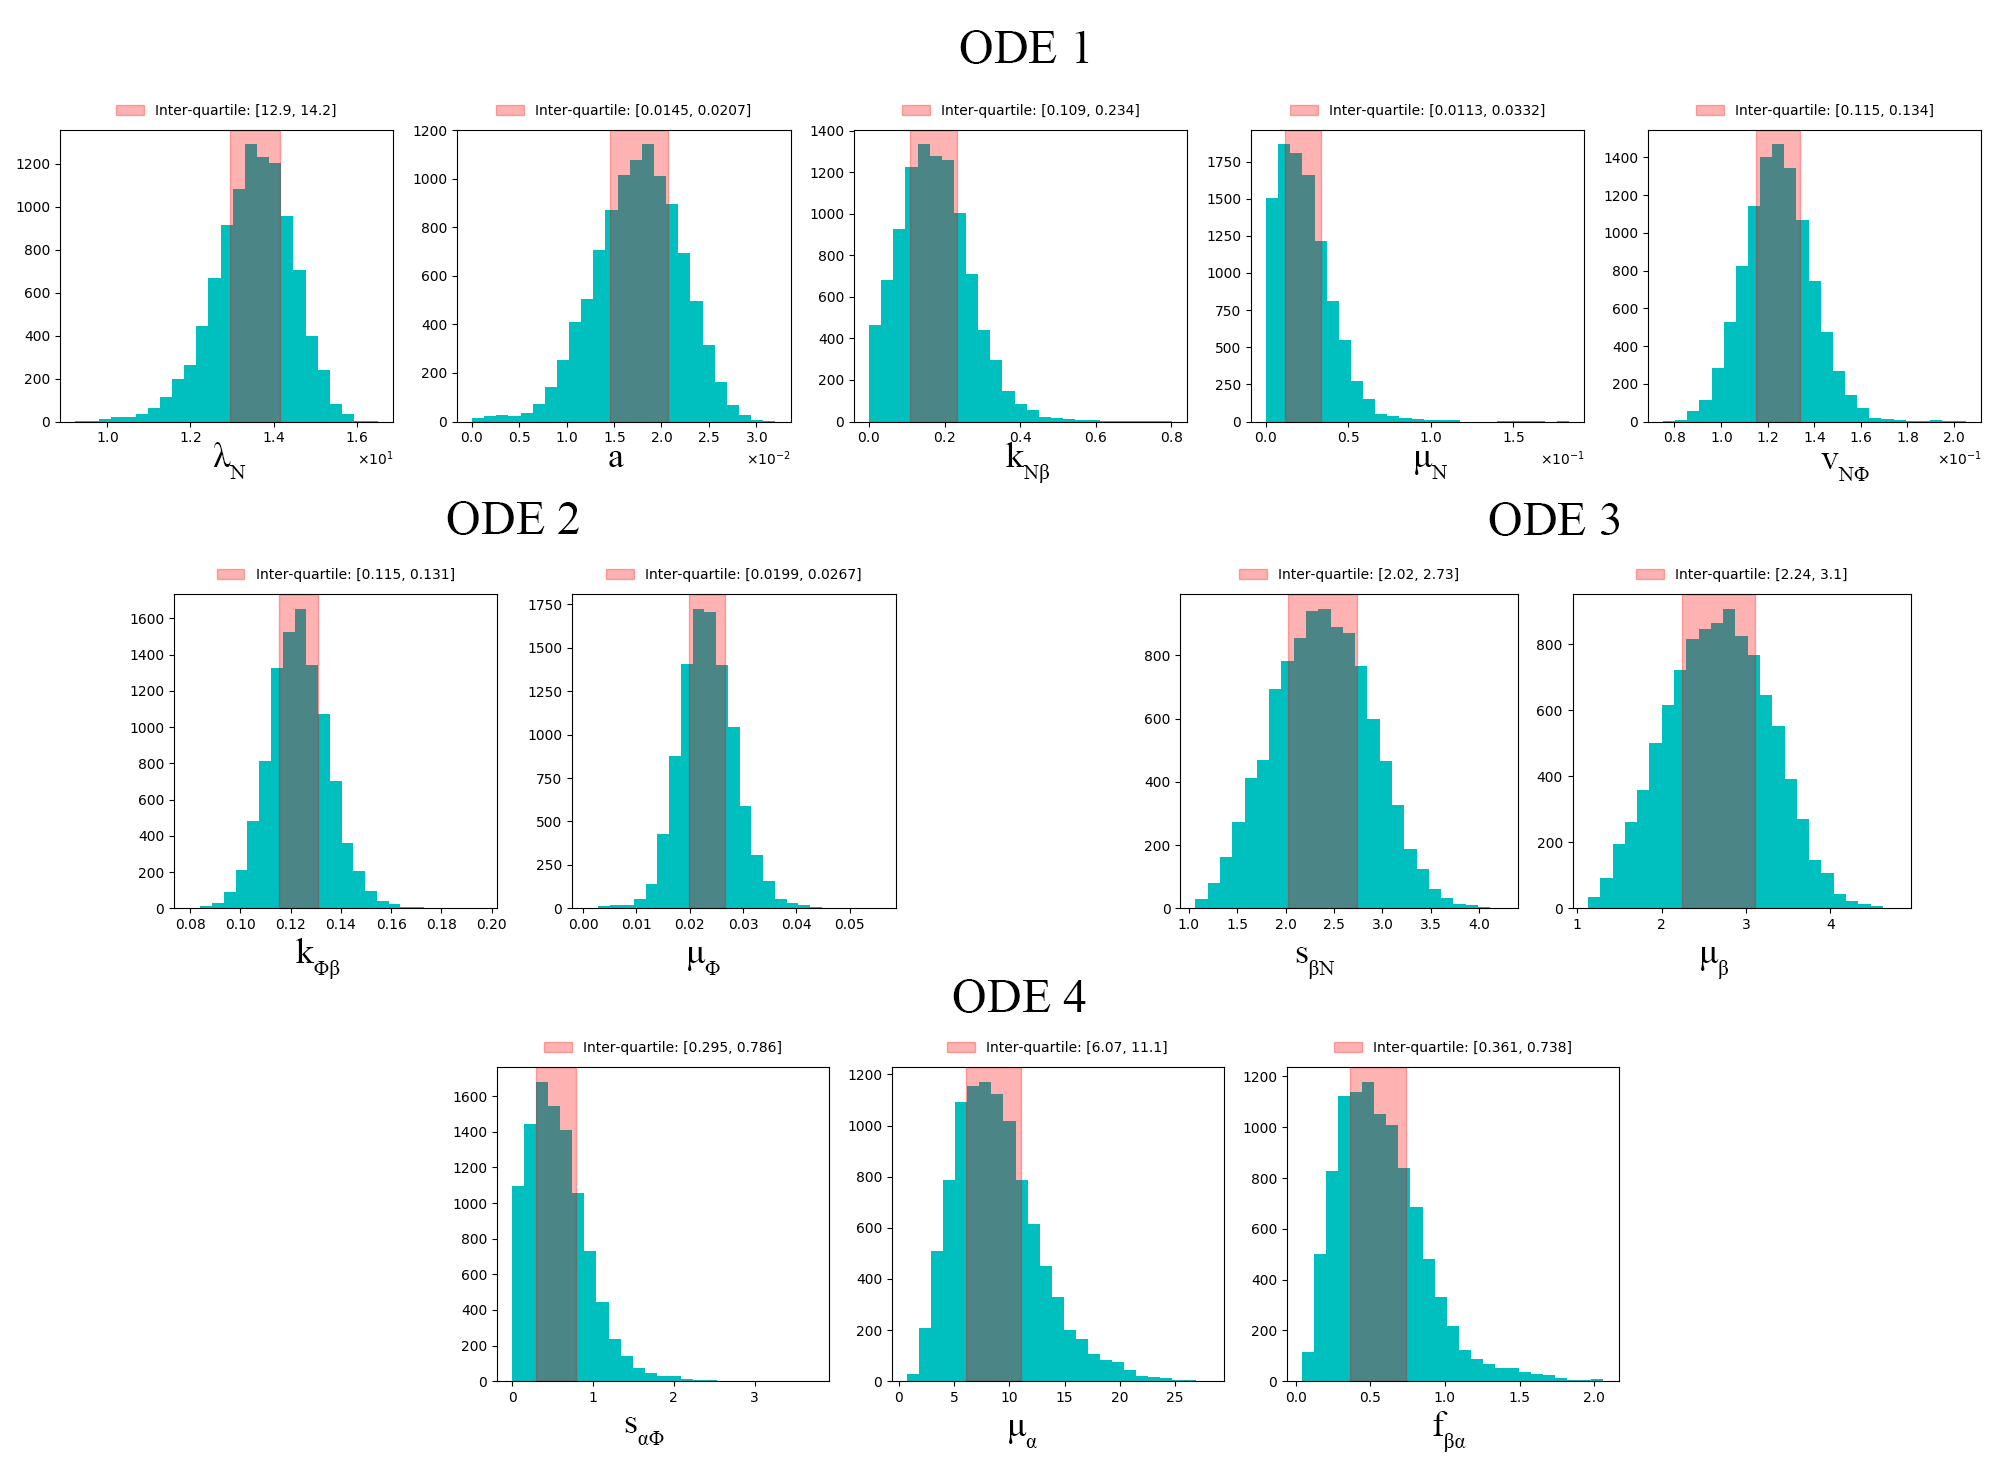
\includegraphics{fig/model5_para.png}}
    \end{center}

    \caption[Inferred posterior distribution of parameters in model 5]%
    {Inferred posterior distribution of parameters in model 5. Shaded range indicates 25\%--75\% quantile of the population}
    \label{fig:model5_para}

\end{figure}

\begin{table}[H]
    \centering
    \begin{tabular}{|c c c|}
        \hline
        Parameter            & Mean value & Inter-quartile interval \\[0.5ex]
        \hline\hline
        $\lambda_N$          & 13.5       & [12.9, 14.2]            \\
        $a$                  & 0.0175     & [0.0145, 0.0207]        \\
        $\kappa_{N\beta}$    & 0.176      & [0.109, 0.234]          \\
        $\mu_N$              & 0.0239     & [0.0113, 0.0332]        \\
        $\nu_{N\Phi}$        & 0.125      & [0.115, 0.134]          \\
        \hline
        $\kappa_{\Phi\beta}$ & 0.123      & [0.115, 0.131]          \\
        $\mu_\Phi$           & 0.0234     & [0.0199, 0.0267]        \\
        \hline
        $s_{\beta N}$        & 2.38       & [2.02, 2.73]            \\
        $\mu_\beta$          & 2.67       & [2.24, 3.10]            \\
        \hline
        $s_{\alpha\Phi}$     & 0.574      & [0.295, 0.786]          \\
        $\mu_\alpha$         & 8.91       & [6.07, 11.1]            \\
        $f_{\beta\alpha}$    & 0.577      & [0.361, 0.738]          \\
        \hline
    \end{tabular}
    \caption[Inferred parameter values of model 5]
    {Inferred parameter values of model 5}
    \label{table:estimated5}
\end{table}


\subsection{Sensitivity of parameters}

% [why last PCs]

% [which parameters are most sensitive]

% [compared to credible intervals plot]

% [what does that mean]

A quick sensitivity analysis of the dynamical systems models can be quantified using principle component analysis (PCA) \cite{Toni}, where the first PCs corresponds to sloppy parameters while the last PCs corresponds to stiff parameters \cite{sensitivity}. PCA can only provide rough approximated sensitivity behaviour. By identifying the component loadings, the PCs can be visualised in pie charts and used to indicate the sensitivity. 

\begin{figure}[H]
    \begin{center}
        \resizebox{1.0\hsize}{!}{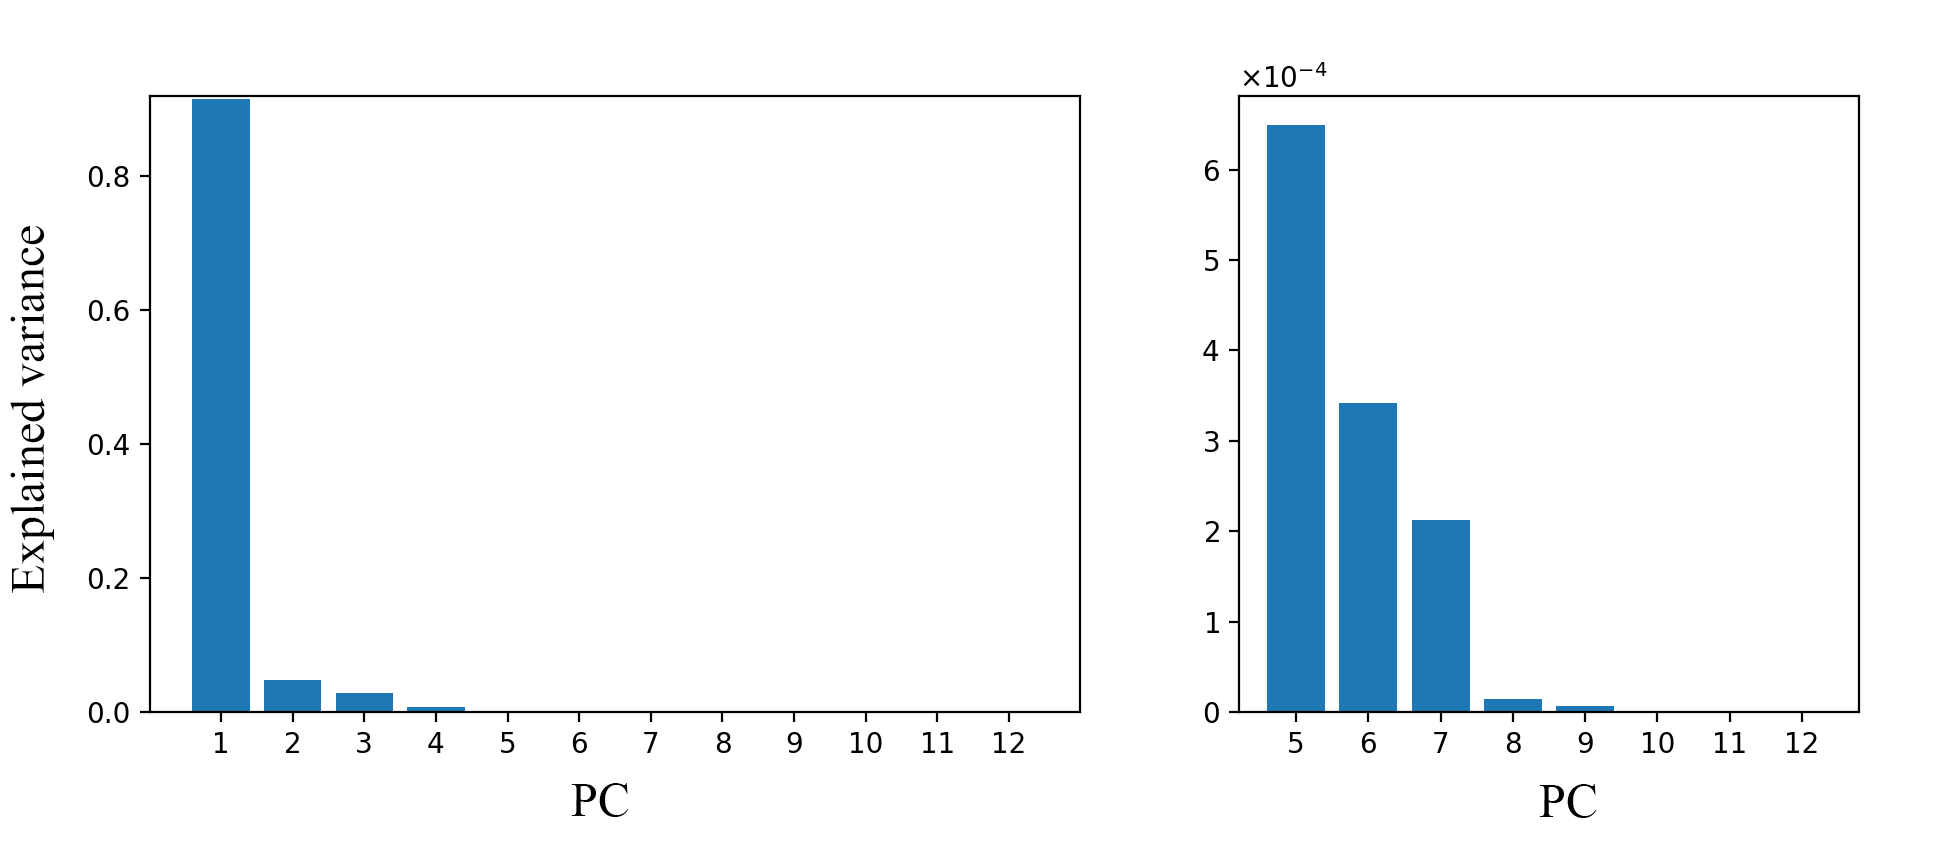
\includegraphics{fig/pc.png}}
    \end{center}

    \caption[Explained total variance in original parameters by each PC]{Explained total variance in original parameters by each PC. From PC 5 on. little variance is explained by each PC, which is enlarged in Right}
    \label{fig:pc}
\end{figure}

\begin{figure}
    \begin{center}
        \resizebox{0.8\hsize}{!}{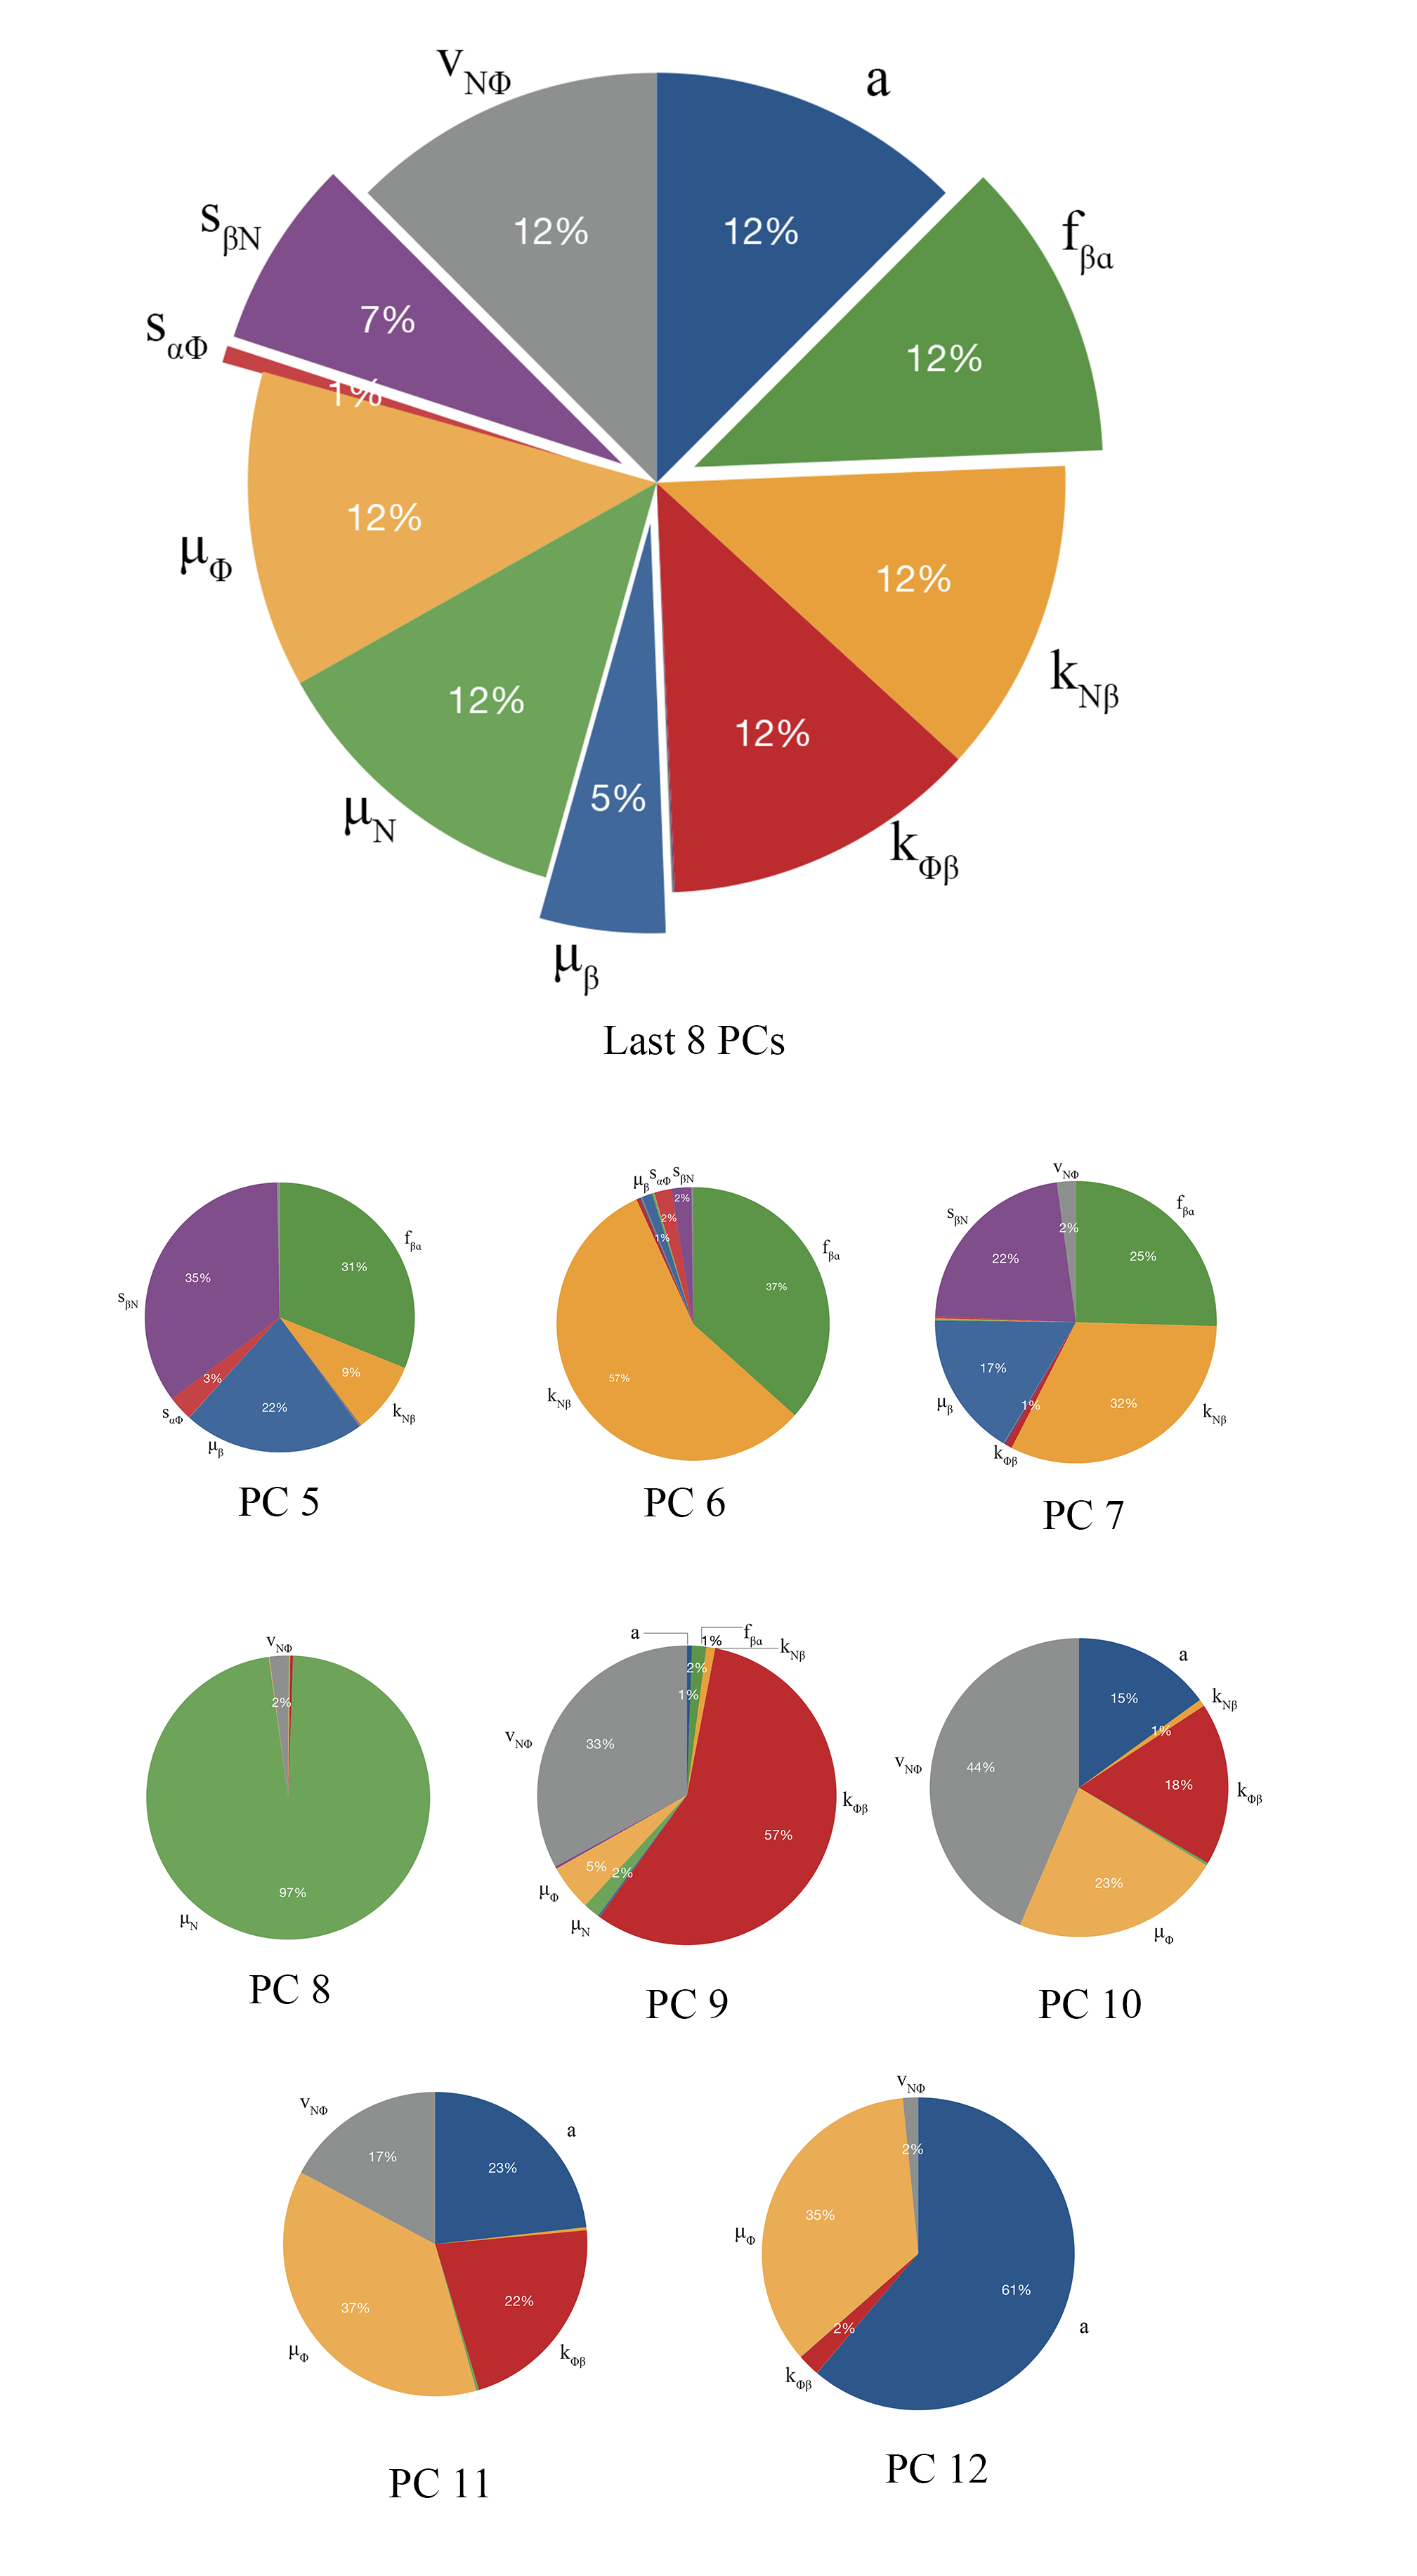
\includegraphics{fig/pc_pie_all.png}}
    \end{center}

    \caption[TODO]{Fraction of the length of PCs explained by parameters}
    \label{fig:pc_pie}
\end{figure}

As models 5 won in the model selection, a further interest was to explore the parameter-to-model sensitivity of the resultant model. PCA was performed on the last generation of inferred model 5, Figure \ref{fig:pc} shows the total explained variance by each PC. The first PC explained a major part of the variance (91.5\%), and the rest PCs explained less less than 5\% of the variance each. PC 5 to PC 12 explained much less variance (less than 0.1\% of the total variance) than the first four PCs, thus they were consider to extend much narrower regions on the posterior distributions and could be used to identify parameter that the model is sensitive to.

Figure \ref{fig:pc_pie} shows the fractions of the PCs explained by individual parameters, and a sum of the fractions in the last 8 PCs, i.e. PC 5 to PC 12. The last PC (PC12) is mostly the linear combination of $a$ (from the equation of neutrophil) and $\mu_\Phi$ (from the equation of macrophage), to which the model is most sensitive. If we conclude the last 8 PCs, it can be found that the biggest portions ($v_{N\Phi}$, $a$, $\kappa_{N\beta}$, $\kappa_{\Phi\beta}$, $\mu_N$, $\mu_\Phi$, $\nu_{N\Phi}$) mostly come from the equation of neutrophil and macrophage i.e. equations of the cells (the un-exploded portion in Figure \ref{fig:pc_pie} a); if we look at the last 8 PCs individually, the same pattern can be observed. This might suggest that the model is more sensitive to cells' dynamic rather than cytokines' dynamics.

The credible intervals (Figure \ref{fig:credible}) of each parameter across generations also agreed with the above conclusion from PCA. The stiff parameters, e.g. $a$ and $\mu_N$, extend narrow credible intervals, while sloppy parameters, e.g. $\mu_\alpha$ and $s_{\alpha\Phi}$, have wider credible intervals across the last few generations.

% then $v_{N\Phi}$, $\mu_N)$ (from the equation of neutrophil) and $k_{\Phi\beta}$ (from the equation of macrophage) contribute most portions together with $a$ and $\mu_\Phi$. As a conclusion, model 5 is sensitive to changes in the above parameters, which all come from the equation of neutrophil and macrophage i.e. equations of the cells; it may suggests that given the observed data, the inferred model is more sensitive to cells' dynamic rather than cytokines' dynamics.

% Also, some visualisations of the last population agreed with conclusions from PCA. Approximated posteriors of the last population plotted in FIGURE and credible ranges of parameters across populations in FIGURE shows that the 5 parameters identified by PCA is indeed `stiff' parameters.


\chapter{Performance experiments}

The performance experiments were designed to explore the parallel performance of ABC SMC inference framework that was used in our parameter estimation and model selection tasks. Generally, ABC SMC is a time-consuming and computation-intensive task and ideally executed on large clusters. The scheduling strategy, implementation details, randomness in the algorithm and many other factors can affect the parallel efficiency. Thus, we designed a scaling-up experiment and studied a case where abnormal performance was observed.

% [MORE meanings of the performance study]

\section{Scaling-up}

First experiments are designed to illustrate the scaling-up performance. The program used here is an implementation of ABC SMC on model 5. The details of the ABC SMC settings are listed below

\begin{itemize}
    \item Prior distribution: default to log-uniform distribution [$1\times 10^{-6}$, 50] for all the 12 parameters
    \item threshold schedule: median epsilon
    \item No factors, no adaptive distance or adaptive population applied
    \item Population size is 2000, with 20 generations
\end{itemize}

% [HOW PYABC parallelise the sampling]

For HPC systems like Cirrus, \verb|pyabc| uses \verb|multiprocessing| for multi-core parallel sampling. By default, if the number of cores is not specified, it will automatically read the number of available cores and use them all. Cirrus has a 36-core CPU which support hyperthreading, such that the maximal number of cores available to \verb|multiprocessing| is 72.

The experiment was executed on Cirrus, using 8, 16, 24, 36, 54 and 72 cores respectively. Each run was repeated ten times and the average execution time, required sampling numbers are recorded. Hyperthreading was enabled when using 54 and 72 cores. The access to the node that contains computation cores is exclusive, such that the execution would not be affected by other programs of operations.

The implementation of ABC SMC in \verb|pyabc| enables the parallelisation of sampling, which is the most time-consuming part. The rest part of the program is mostly not parallelised, e.g. database I/O and reductions operations. The sampling process involves sampling, perturbation and test of the acceptance criteria, which are computation-intensive.

In practice, using ABC SMC to estimate the parameters of a given model could cost up to several hundred of hours if the computational resources are limited \cite{ref:compare}. The performance experiment result could provide a reference that illustrates how the efficiency changes when scaling-up or the trade-offs in computational resources' cost and their benefit.

\subsubsection{Results}

% [scaling-up performance: speed-up and efficiency]

% [large variation in required sampling numbers]

% [possible reasons]

\begin{figure}[h]
    \begin{center}
        \resizebox{1.0\hsize}{!}{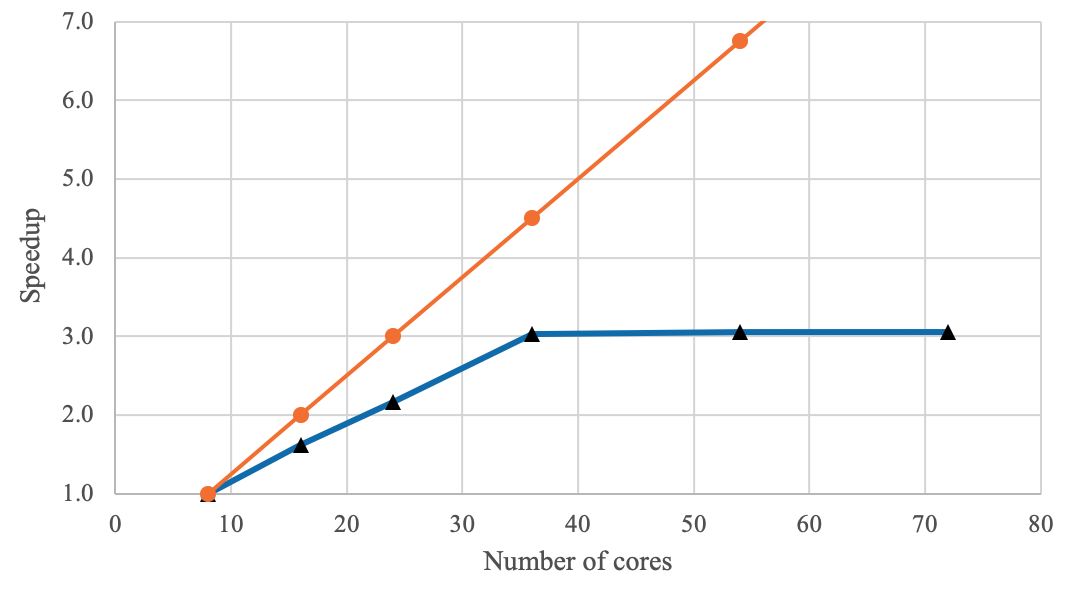
\includegraphics{fig/speedup.png}}
    \end{center}

    \caption[Speedup of the program]{Speedup of the program. Line in orange indicates the ideal linear speedup}
    \label{fig:speedup}
\end{figure}

The recorded execution time under different numbers of cores was used to calculate the speedup of the program (Figure \ref{fig:speedup}). Here 8-core run is regarded as the baseline for speedup and efficiency, as the serial version (using only one core) can take quite a long time to finish 10 repeats. When increasing number of cores, the execution time drops fast at first, but the decreasing trend became slower for large numbers of cores; 36, 54 and 72 cores gives nearly the same average execution time and consequently gains very close speedup values (Table \ref{table:performance}).

\begin{table}[H]
    \centering
    \begin{tabular}{|c c c c c|}
        \hline
        Number of cores & Avg. time (second) & Avg. sample size & Speedup & Efficiency \\ [0.5ex]
        \hline\hline
        8               & 6617          & 445406.8              & 1       & 1          \\
        16              & 3926          & 590221.0              & 1.61    & 0.807      \\
        24              & 2921          & 573339.8              & 2.17    & 0.723      \\
        36              & 2096          & 446948.7              & 3.02    & 0.672      \\
        54              & 2076          & 640404.9              & 3.05    & 0.452      \\
        72              & 2071          & 768096.0              & 3.06    & 0.340      \\
        \hline
    \end{tabular}
    \caption{Performance data}
    \label{table:performance}
\end{table}

Denote the number of cores used in the ABC SMC runs as variable $p$. The speedup curve shows a linear trend when $p\leq 36$; when $p\geq 36$ the speedup stays nearly unchanged. $p=36$ is an inflexion point, where 36 is the maximum numbers available physical cores in a compute node of Cirrus. A constant drop of efficiency is observed when increasing $p$; smaller $p$ ($p<36$) gives an efficiency higher than 65\% but greater $p$ e.g. $p=72$ results in a low efficiency (34\%).

% \begin{figure}[h]
%     \begin{center}
%         \resizebox{1.0\hsize}{!}{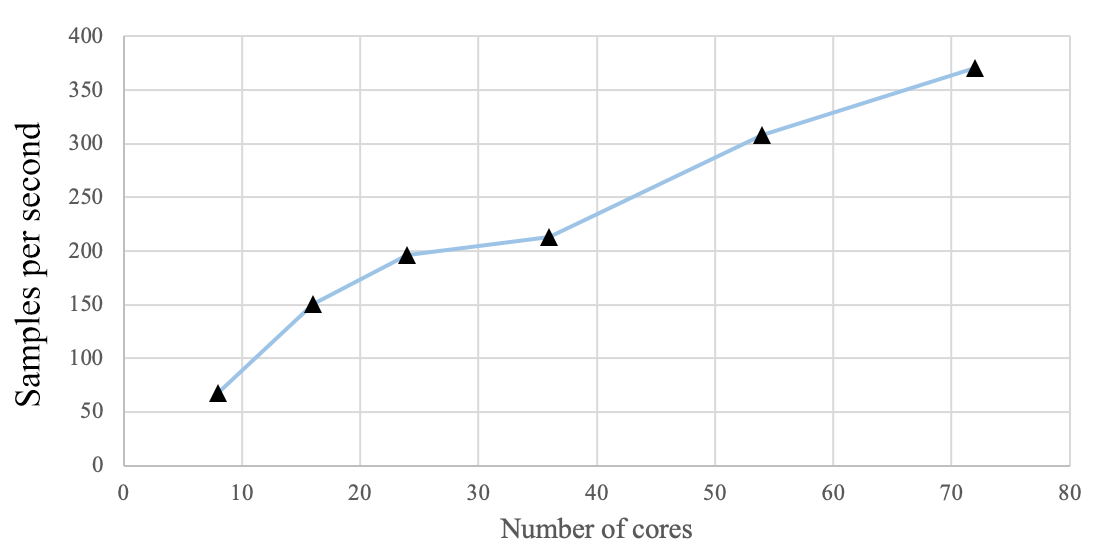
\includegraphics{fig/sample_per_time.png}}
%     \end{center}

%     \caption[Average samples in a second, under different number of cores]{Average samples in one second, under different number of cores}
%     \label{fig:sample_per_sec}
% \end{figure}

\section{Discussions}

A high variance of total required samples was observed in the scaling-up experiments: some single runs required much more samples to finish 20 populations, where they were supposed to have relatively similar average required samples such that we can compare the performance directly via speedup or efficiency. 

Due to the variant total required samples drawn our attention to the per-second performance. Although the execution time was not improved by using 54 or 72 cores, the required number of samples were higher than that of $p=36$, which indicates slight improvements. However, the high variance made us hard to gave statistically significant conclusions on the per-second performance.

% our interests switched to the per-second performance, where the average sampling numbers per second under different of numbers of cores ($p$) are plotted (Figure \ref{fig:sample_per_sec}). The plot shows that even theoretical speedup stops growing when $p>36$, the average sampling numbers per second performance still get improved when using more than 36 cores. It proves that the implementation used here scales reasonably well without encountering bottleneck when using multi-core parallelisation inside one physical node.

The variant total required samples for different runs under the same setting was most likely the result of different threshold evolve path. Median epsilon schedule and randomness in the sampling process resulted in different sequences of thresholds for different runs, which means different repeated runs may have different convergency path \cite{threshold}. For example, Some runs temporarily converge to a local optimum, while the target epsilon in the next generation cannot possibly be reached if the new particles are still concentrated in the local optimum. In this case, a huge amount of sample will be drawn to find enough accepted particles, and the new generation will be able to jump out of the local optimum and have different concentrations. 

\begin{figure}[ht!]
    \begin{center}
        \resizebox{1.0\hsize}{!}{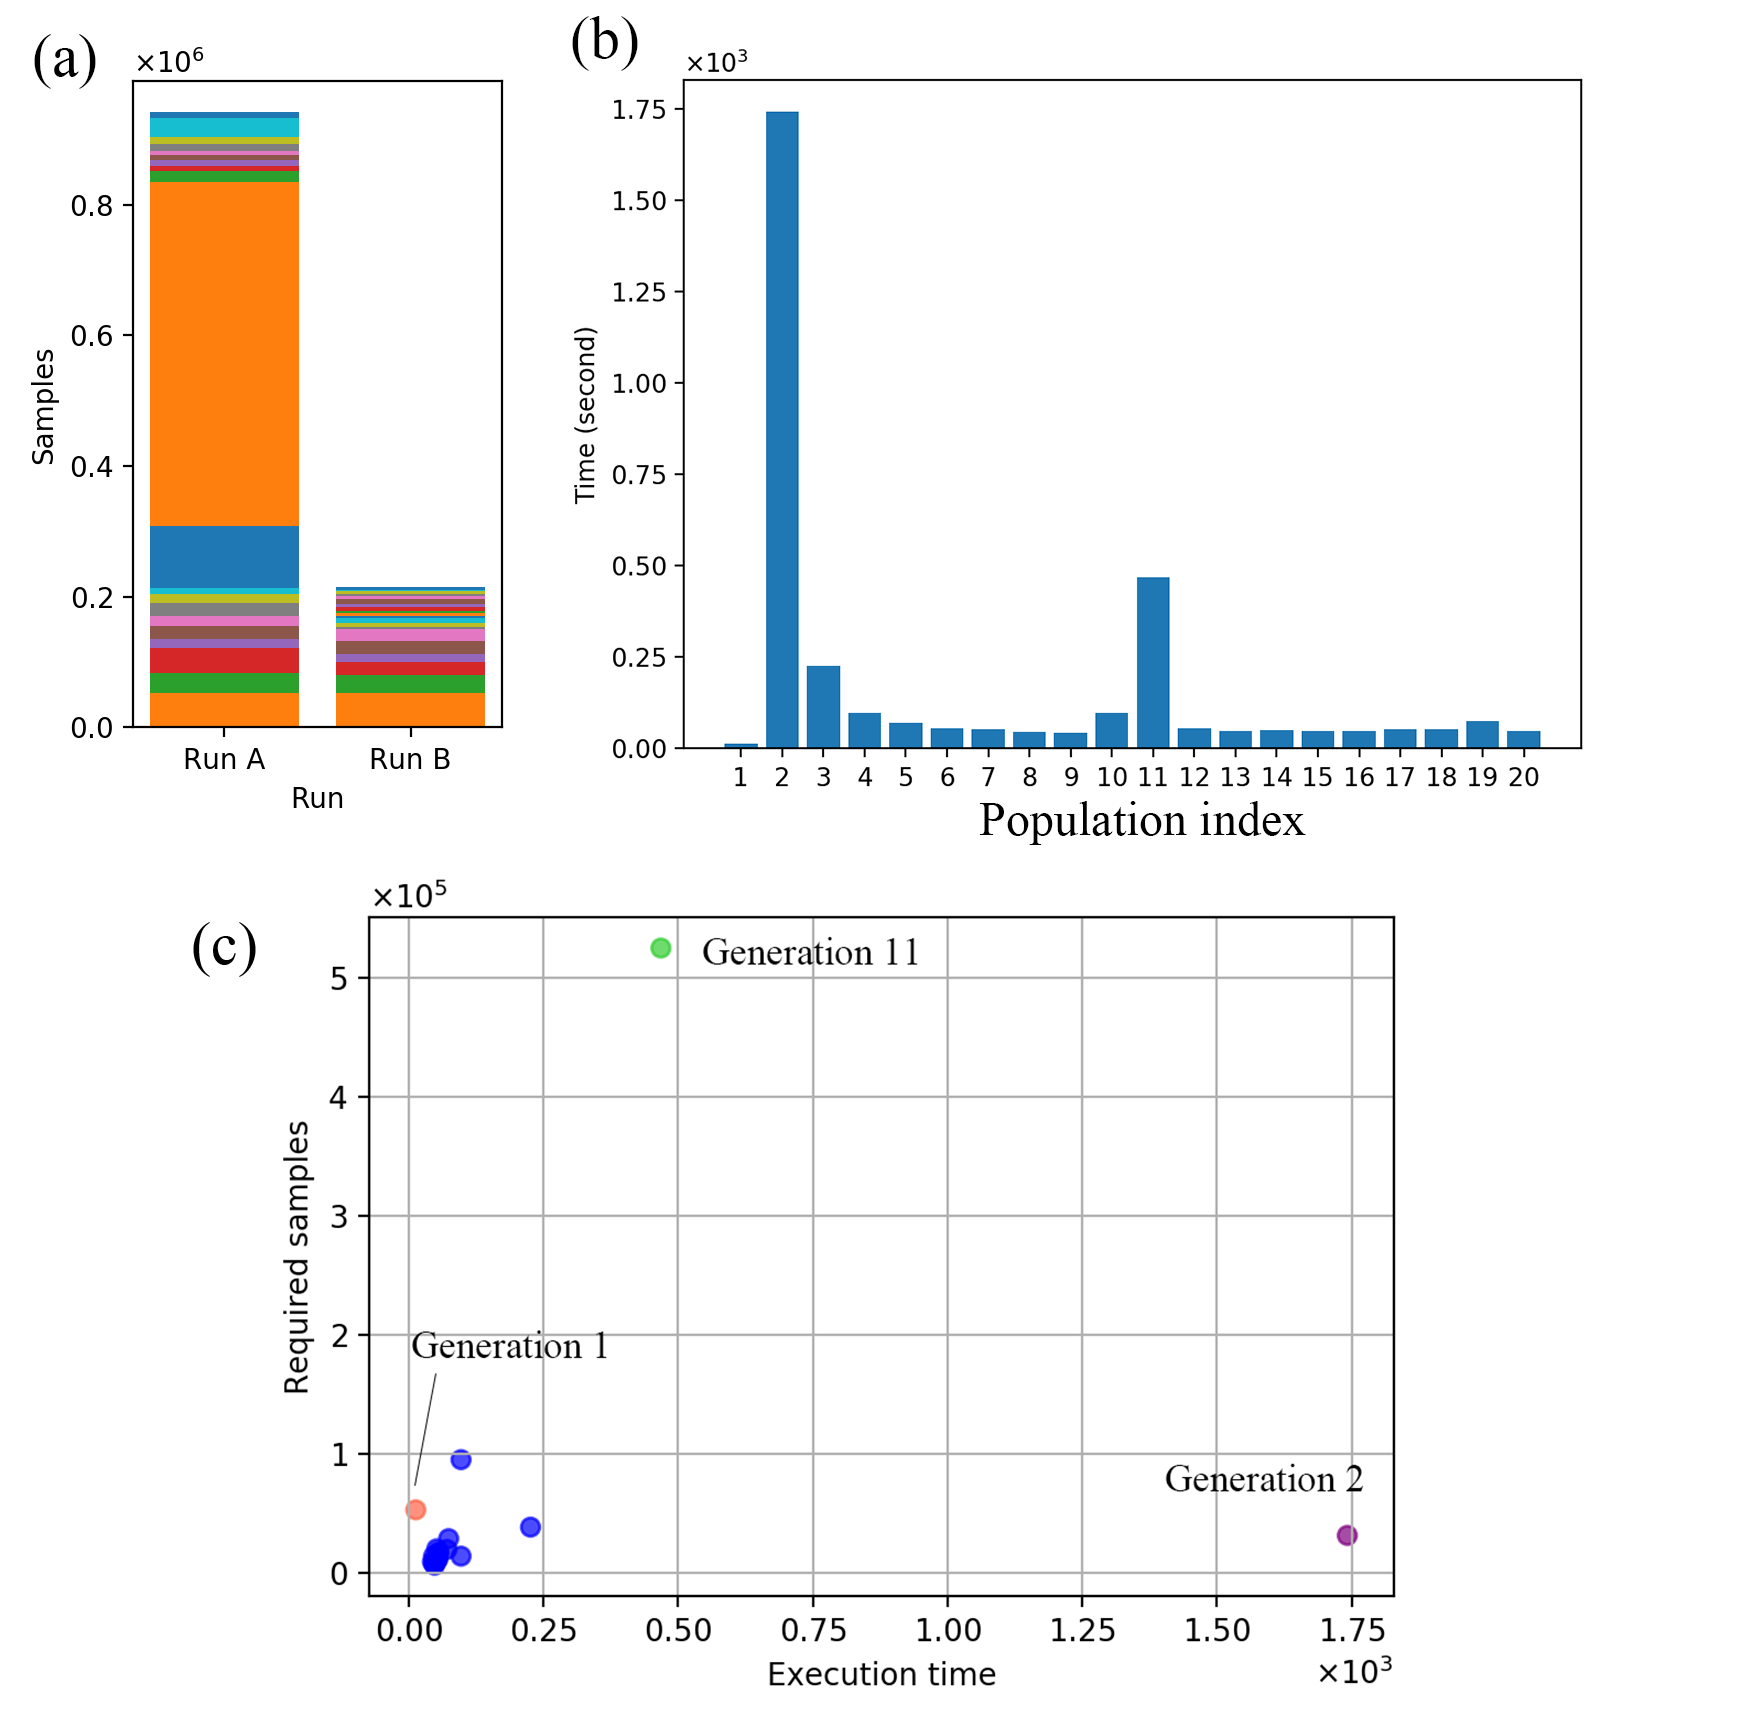
\includegraphics{fig/local_modes_new.png}}
    \end{center}

    \caption[Local optimum and abnormal pattern]{(a) Required number of samples for two example runs (A and B). Different colour represents different generation (from bottom to top: generation 1 to generation 20). Run A took huge amount of time in population 11. (b) Execution time for each generation of Run A. (c) Scatter plot of required number of samples against execution time for each generation. Generation 1 and two outliers, i.e. generation 11 and generation 2, are marked in different colours from other generations}
    \label{fig:local_modes}
\end{figure}

To illustrate this, Two independent run, namely Run A and Run B, were chosen from the experiment of $p=24$ and visualised in Figure \ref{fig:local_modes} and Figure \ref{fig:local_para}. These two runs used identical options of the algorithm. Figure \ref{fig:local_modes} (a) shows the comparison of the required samples, where Run A converged to a local mode, and in population 11 took much more sample tires to move away from the local optimum (Figure \ref{fig:local_modes} (b)). Figure \ref{fig:local_para} compares the posterior density distribution before (t=9, cyan) and after (t=13, red) the jumping away: significant movement of concentrations in posterior density distributions are observed, especially in parameters from ODE 1, 2 and 4. An interning movement is that there are two concentrations in $\kappa_{\Phi\beta}$ and $\mu_\Phi$ when t=9, and the majority of particles are concentrated in the second concentration with high parameter values; when t=13, the second concentration distribution disappears and all particles are concentrated near zero.

\begin{figure}[ht!]
    \begin{center}
        \resizebox{1.0\hsize}{!}{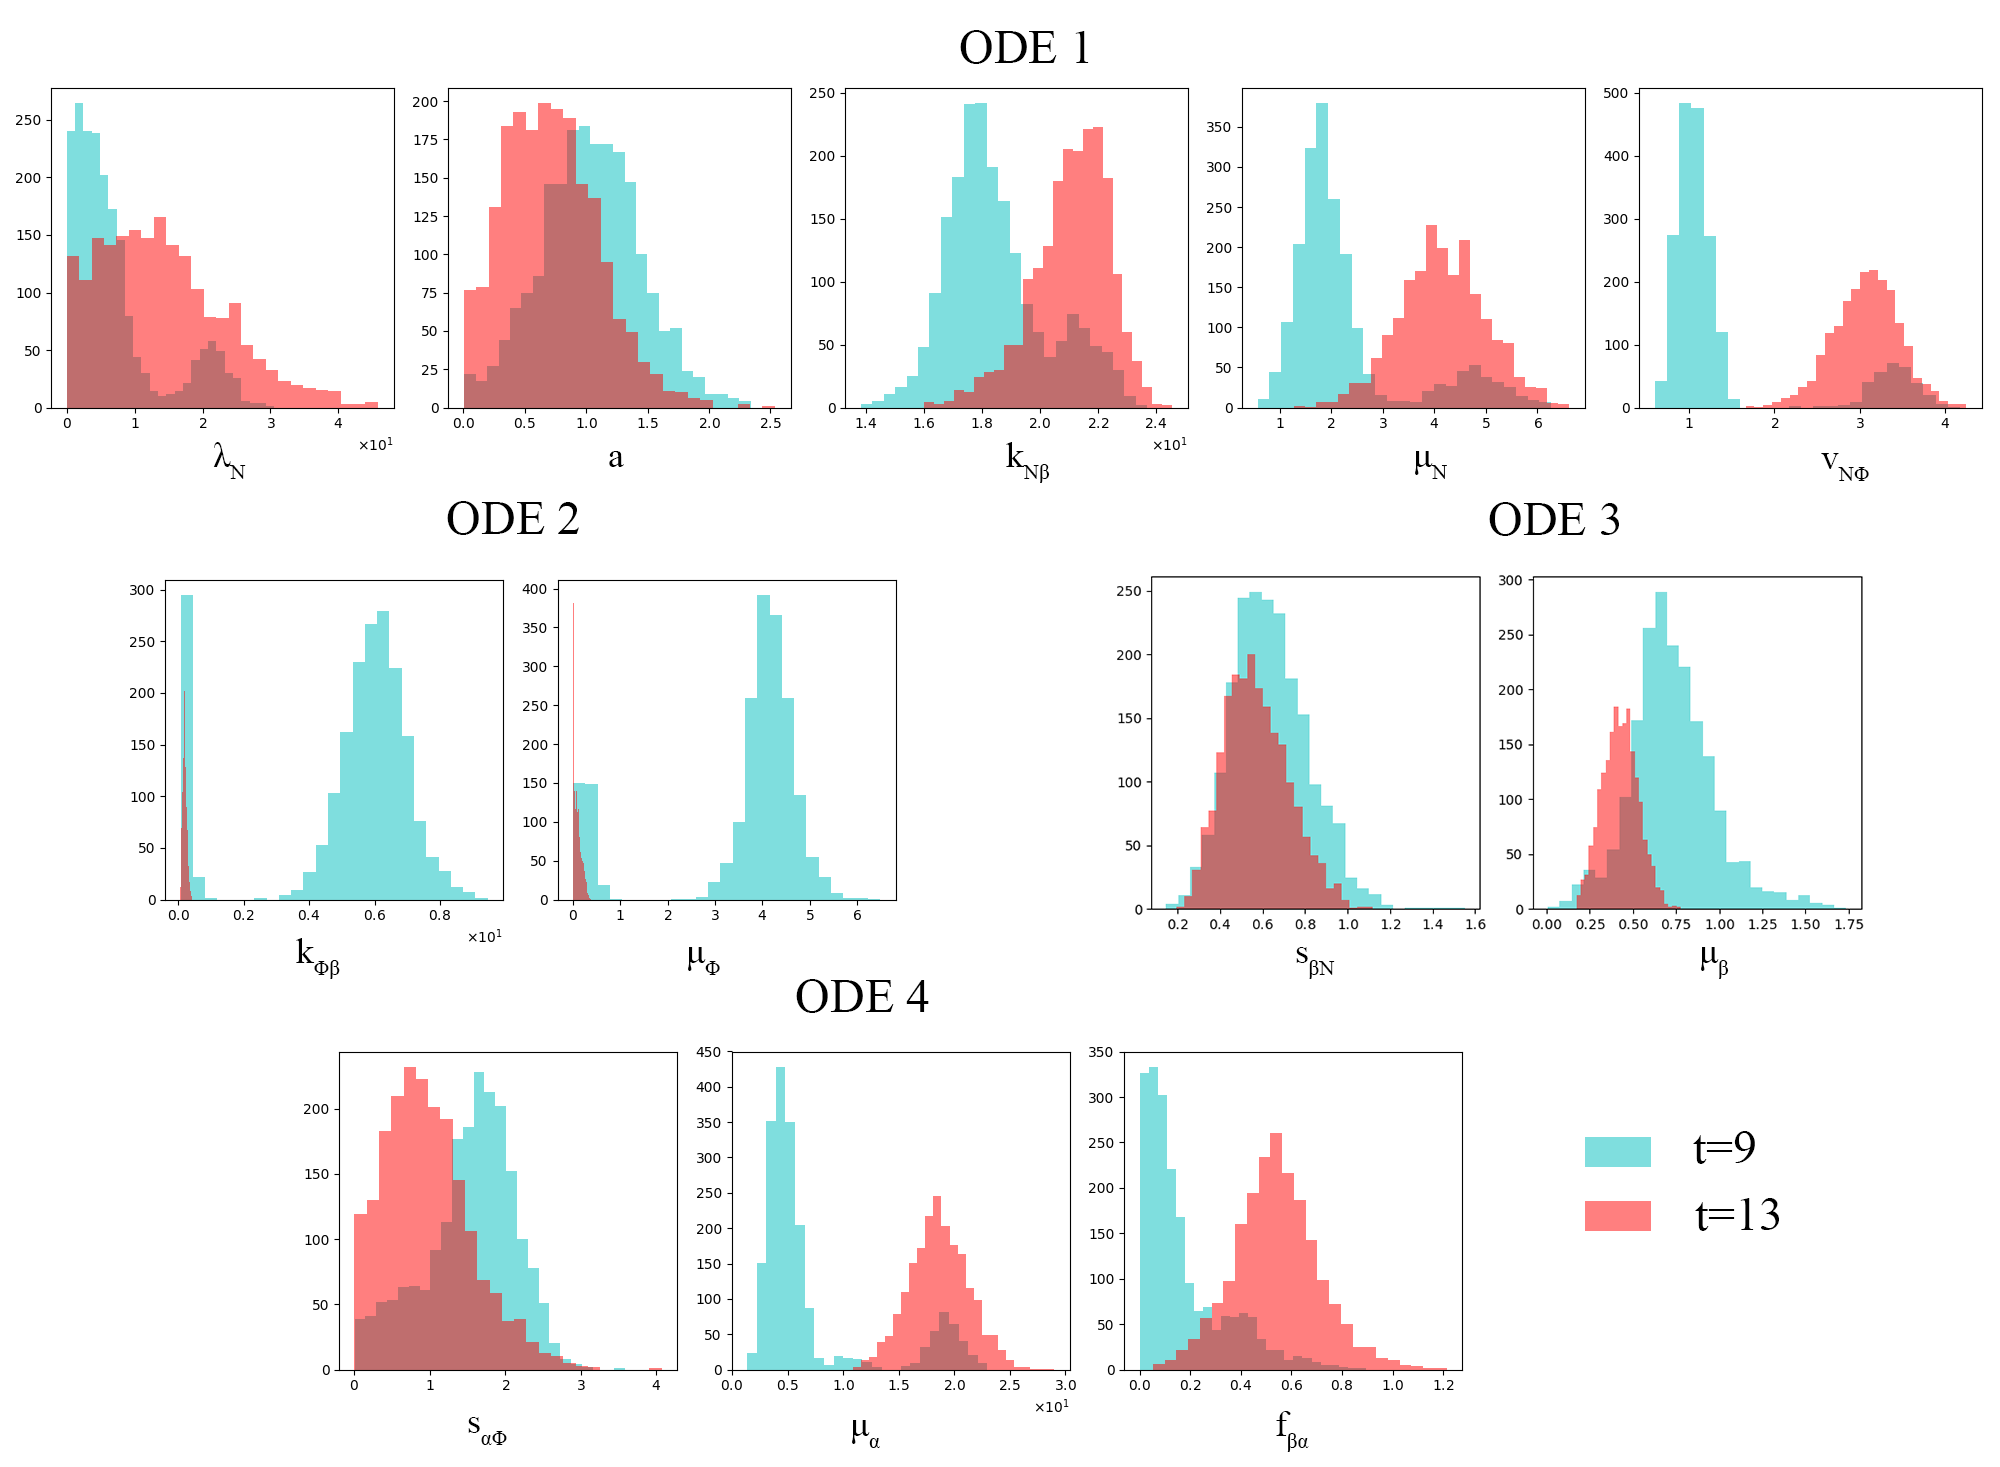
\includegraphics{fig/local_para.png}}
    \end{center}

    \caption[Parameter density distribution before and after the concentration movement in generation 11]{Parameter density distribution before (generation 9, cyan) and after (generation 13, red) the concentration movement in generation 11}
    \label{fig:local_para}
\end{figure}

Moreover, we found that the execution time was not ideally proportional to the sampling tires in that period of time, for both different repeated runs and different generations in a single run. From the same example, the sample size for each generation of Run A (Figure \ref{fig:local_modes} (a)) is not proportional to its execution time (Figure \ref{fig:local_modes} (b)), especially for the first two generations and generation 11. Figure \ref{fig:local_modes} (c) shows a scatter plot of the required samples and execution time for each generation, where two obvious outliers (generation 1 and generation 11) are observed.

% Figure \ref{fig:local_modes} (b) and (c) show the non-linear relationship between execution time and sample tries in different generations. 

% Apart from 1st and 2nd generation, generation 3 to 20 show a general linear relationship i.e. $T_t\propto n_t$, where $t$ is the population index, $T_t$ is the execution time of generation $t$ and $n_t$ is the required samples in generation $t$.

% However, this relationship does not hold for the first two generations. 

Generation 1 (red pont in Figure \ref{fig:local_modes} (c)) drew samples from prior, but it was done with high efficiency as only a small amount of time are taken; generation 2 (purple pont in Figure \ref{fig:local_modes} (c)) took an unusually large amount of the while it did not require much more samples. The abnormal execution time of generation 1 and 2 were observed in all other runs, where for $p=24$ generation 1 usually takes c. 16s and generation 2 takes c. 1600s. This is believed to be related to the initialisation of the algorithm. For local modes, e.g. generation 11 (green pont in Figure \ref{fig:local_modes} (c)), high efficiency were achieved.

By looking into the code, some reasons can be found. There exist some `cheap' particles. If at the first time points, a variable reached unacceptable high value (regarded as \verb|Inf| in \verb|Python|), the ODE solver cannot perform further integration but result in a data full of \verb|NaN|s. Such particles cost less time than an usual particle (where values at 120 data points are explicitly calculated and then compared with observed data). Local mode, e.g. generation 11, might take large amount of these `cheap' particles. Also, generation 1 draws samples directly from prior without fitting and using kernels, so it is much faster. The huge amount of time observed in generation 2 is believed to be a result of some initialisation steps in the ABC SMC algorithm.

To conclude, the performance experiments revealed reasonable scaling-up behaviour when the \verb|Python| processes did not exceed number of physical cores. Local modes lead to high variance in total required number of samples, and the relationship between required sample numbers and required execution time are not ideally linear; they all made further detailed analysis difficult.

Additionally, by observing CPU frequency and load curve in-time while running the program, we found that the parallelised part is limited to the sampling, calculation and criterion test process. Some reduction calculations and preparation work for the next generation (e.g. calculation of the new epsilon values, normalisation of data, fit of multivariate kernel) are serial. The database I/O is also serial.  It is noticed that the program took no advantage of graphics card, as \verb|multiprocessing| along can only exploit the resources inside CPU. 

% A possible explain to these phenomenons can be that the median epsilon schedule results in different threshold strategies due to the randomness in the sampling process, thus results in different approximate convergency paths for different runs. Some runs that are stuck in a local optimum and require smaller target epsilon will take huge amount of samples to move away from the local optimum. This have been observed when the distribution of posterior is plotted before and after jumping away from local modes (FIGURE and more explain). Also, time spent in each sample using sanme number of cores is not constant in our case, which might be a result of the parallel schedule; ideally a serial run using only one core will see a nearly constant time spent in every particle.



% \section{Profiling}

% The performance could also be analysed given a profiling report. The second experiment profiles the program to reveal the detailed time consumption for each operation and the possible bottleneck, according to which we could find the hot-spot of program and given possible suggestions on improving the performance.

% In this case, profile tools \verb|cProfile| and \verb|yappi| is used in PyCharm IDE.

% \subsubsection{Results}

% [profiling results: hot-spot and possible improvements]


\chapter{Conclusion and future works}

%  [what is studied]

%  [to what extend]

%  [how good is the result]

 To conclude, ABC SMC was successfully applied to the models of zebrafish spinal cord regeneration. These models were all ODE equations that described the interactions and effects between cells and proteins in the lesion site. These equations contain four dependent variable and more than 10 model parameters.  Parameter estimation for high-dimensional parameter space is a challenging work for many dynamic system models, as insufficient explore of parameter space can easily lead to local optimal. Using a large population size in ABC SMC in our models could partially relief the concerns in local modes, and give considerable parameter estimates. We found that the first three models could not recover some local features observed in the early times, so further models -- model 4 and 5 -- were proposed. Additional interactions were introduced in the new model, and the results proved that they were helpful in resolving the under-fit.
 
 Also, ABC SMC successfully helped in the model comparison and thus can be used for suggestions of the best model, although there were uncertainties remained in the process and a large number of population size needed. In our practice, model 5 won with absolute advantages when the threshold is converged to a small value. The approximated posteriors showed bell-shaped density distribution for most of the parameters (Figure \ref{fig:model5_para} and Figure \ref{fig:para1}), indicating that most parameters were well-inferred in our implementations.

%  ABC SMC implementation is a complex process with respect to both algorithm settings and code development. The ability of parameter inference and robustness of algorithm was firstly studied using synthetic data where the true parameter value was known, and experiments were performed to find proper hyperparameter and implementation settings of ABC SMC. 

% Later inference on the observed data followed these suggestions from the synthetic data experiments and acceptable results were produced. These examples proved that ABC SMC was capable of the inference tasks for the proposed models with high-dimensional parameter space.

 The inference program was mostly run on multi-core machines, and additional scaling-up performance test illustrated the scaling behaviour. When the number of running \verb|Python| process exceeds the number of physical cores, hyperthreading would be enabled, and performance improvement was still considerable (Figure \ref{fig:sample_per_sec}). Studies on the variant required samples revealed that some threshold paths could lead to local optimum and significantly affect the efficiency. A non-linear relationship between the required samples and execution time was also observed in the first two generations.

%  [summary of the findings and advise]

 From this application, some suggestions on ABC SMC implementation could be drawn. How to set the prior could be the most tricky decision for high dimensional parameter inference. The distribution and the interval of each parameter can affect the inference results significantly, and improper prior cold lead to poor fit. In our cases, log-uniform prior gave better fits than uniform prior. The threshold path and plot of required samples in each generation can be used to identify possible local modes; if stuck, it takes much more samples than usual to move out. To avoid this, large population size and a proper epsilon schedule may help. For the uncertainties observed in model selection and some duplicated runs with high variance, a longer run with more generation could help to identify whether the convergency is consistent such that a reproducible inferred results can be obtained.

%  [thanks]

In terms of the future works, some more comparison with other algorisms could be of our interest. Least square fitting using MCMC \cite{ref:MCMC} and some other exact inference approaches could be performed on the same model and observed data, as the standard deviation at each measurement point is known. By comparing to these methods, differences in the inference results, algorithm robustness and required computational resources could be revealed and possibly help us in choosing an inference algorism that can balance the trade-off between efficiency and a reasonable good `fit'. Also there other implementation options of ABC SMC worth trying, e.g. CUDA acceleration and \verb|Julia| implementations\footnote[1]{\url{https://github.com/tanhevg/GpABC.jl}} \footnote[2]{\url{https://github.com/marcjwilliams1/ApproxBayes.jl}}.

In the aspect of models, some further models can be studied. If there were some more experimental evidence on the proposed interaction map, we could propose more precise models, or calibrate some terms in our existing models. Also, models of other forms, e.g. PDE and stochastic models, could also be studied if a more complex model is needed for the dynamic system. Simplification is also possible of existing models. Some highly-correlated parameters could be reduced, as there exist some linear relationships between parameters.  

% Beyond this scope, we are interested in the 

% \chapter{Results and Discussions}

% [WHAT results is outputted and WHAT topics are discussed]

% \section{ABC SMC results}

% [inferred parameters: joint distribution, estimated values and simulated trajectory for each models; sensitivity; features of the inferred model]

% [model selections result; bayes factor]



% \section{Discussions}

% [goodness of fit (evaluation); preferred models and effects of modification to basic model]

% [efficiency and trade-offs in scaling-up]

% [POSSIBLE: compare to exact inference; compared to other implementations]

% [limitations]


\appendix
% the appendix command just changes heading styles for appendices.

\chapter{System and software environment}

\section{ABC SMC implementation}

\subsection{Local machine}

Local development machine is a Mac laptop, running on macOS 10.15.6. The environment of the development is listed in Table \ref{table:local_macine}.

\begin{table}[H]
    \centering
    \begin{tabular}{|c c|}
        \hline
        Environment        & Version                \\ [0.5ex]
        \hline\hline
        Operating system   & macOS Catalina 10.15.6 \\
        PyCharm (IDE)      & Professional 202.2     \\
        Python interpretor & 3.7.0                  \\
        IPython            & 7.12.0                 \\
        Clang              & 6.0 (clang-600.0.57)   \\
        \hline
    \end{tabular}
    \caption{Environment on local machine}
    \label{table:local_macine}
\end{table}

Version requirements for some critical site packages (\verb|Python|) used in the code are listed in Table \ref{table:local_package}.

\begin{table}
    \centering
    \begin{tabular}{|c c|}
        \hline
        Environment & Version         \\ [0.5ex]
        \hline\hline
        pyABC       & $\simeq$ 0.10.3 \\
        NumPy       & $\simeq$ 1.18.4 \\
        SciPy       & $\simeq$ 1.4.1  \\
        pandas      & $\simeq$ 1.1.0  \\
        matplotlib  & $\simeq$ 3.0.1  \\
        bokeh       & $=$ 1.4.0       \\
        \hline
    \end{tabular}
    \caption{Site packages on local machine}
    \label{table:local_package}
\end{table}

Local development and some runs of small size were done under the hardware listed in Table \ref{table:local_hardware}. When running ABC SMC, the program can make used of 8 python process (Hyper-Threading enabled) and run under 3.8GHz (maximal) for a long time under proper cooling, proved that the program could efficiently use the computation resources for a local personal computer. It is noted that the program took no advantage of graphics card, as \verb|multiprocessing| along can only exploit the resources inside CPU. The execution time and other performance data presented in Chapter 5 were obtained using remote machines but not local machine.

\begin{table}
    \centering
    \begin{tabular}{|c c|}
        \hline
        Hardware        & Detail                                \\ [0.5ex]
        \hline\hline
        CPU             & Quad-Core Intel Core i5 8259U 2.3 GHz \\
        Architecture    & 64 Bit                                \\
        Hyper-Threading & Supported                             \\
        Turbo Boost     & Max 3.8 GHz                           \\
        Memory          & 16 GB                                  \\
        Graphics card   & Iris Plus Graphics 655                \\
        \hline
    \end{tabular}
    \caption{Hardwares on local machine}
    \label{table:local_hardware}
\end{table}



\subsection{Remote machine}

\begin{table}[H]
    \centering
    \begin{tabular}{|c c|}
        \hline
        Environment                 & Version                       \\ [0.5ex]
        \hline\hline
        Placeholder                 & 2\\
        \hline
    \end{tabular}
    \caption{Environment on remote machine}
    \label{table:remote_macine}
\end{table}

\section{Data analysis}

\chapter{Data and settings}






\section{Infer-back experiments}

\subsection{Parameter values used to generate synthetic data}

\begin{table}[H]
    \centering
    \begin{tabular}{|c c|}
        \hline
        Parameter            & Value \\[0.5ex]
        \hline\hline
        $\lambda_N$          & 2.20  \\
        $\kappa_{N\beta}$    & 3.96  \\
        $\mu_N$              & 1.72  \\
        $\nu_{N\Phi}$        & 0.219 \\
        \hline
        $\lambda_\Phi$       & 1.31 \\
        $\kappa_{\Phi\beta}$ & 0.124 \\
        $\mu_\Phi$           & 0.145 \\
        \hline
        $s_{\beta N}$        & 6.55  \\
        $i_{\beta\Phi}$ & 1.71 \\
        $\mu_\beta$          & 0.521  \\
        \hline
        $s_{\alpha\Phi}$     & 10.2 \\
        $\mu_\alpha$         & 19.7  \\
        \hline
    \end{tabular}
    \caption[TODO]
    {Known values TODO}
    \label{table:known_values}
\end{table}

\subsection{Kernel experiment: median epsilon schedule}

\begin{figure}[H]

    \begin{center}
        \resizebox{1.0\hsize}{!}{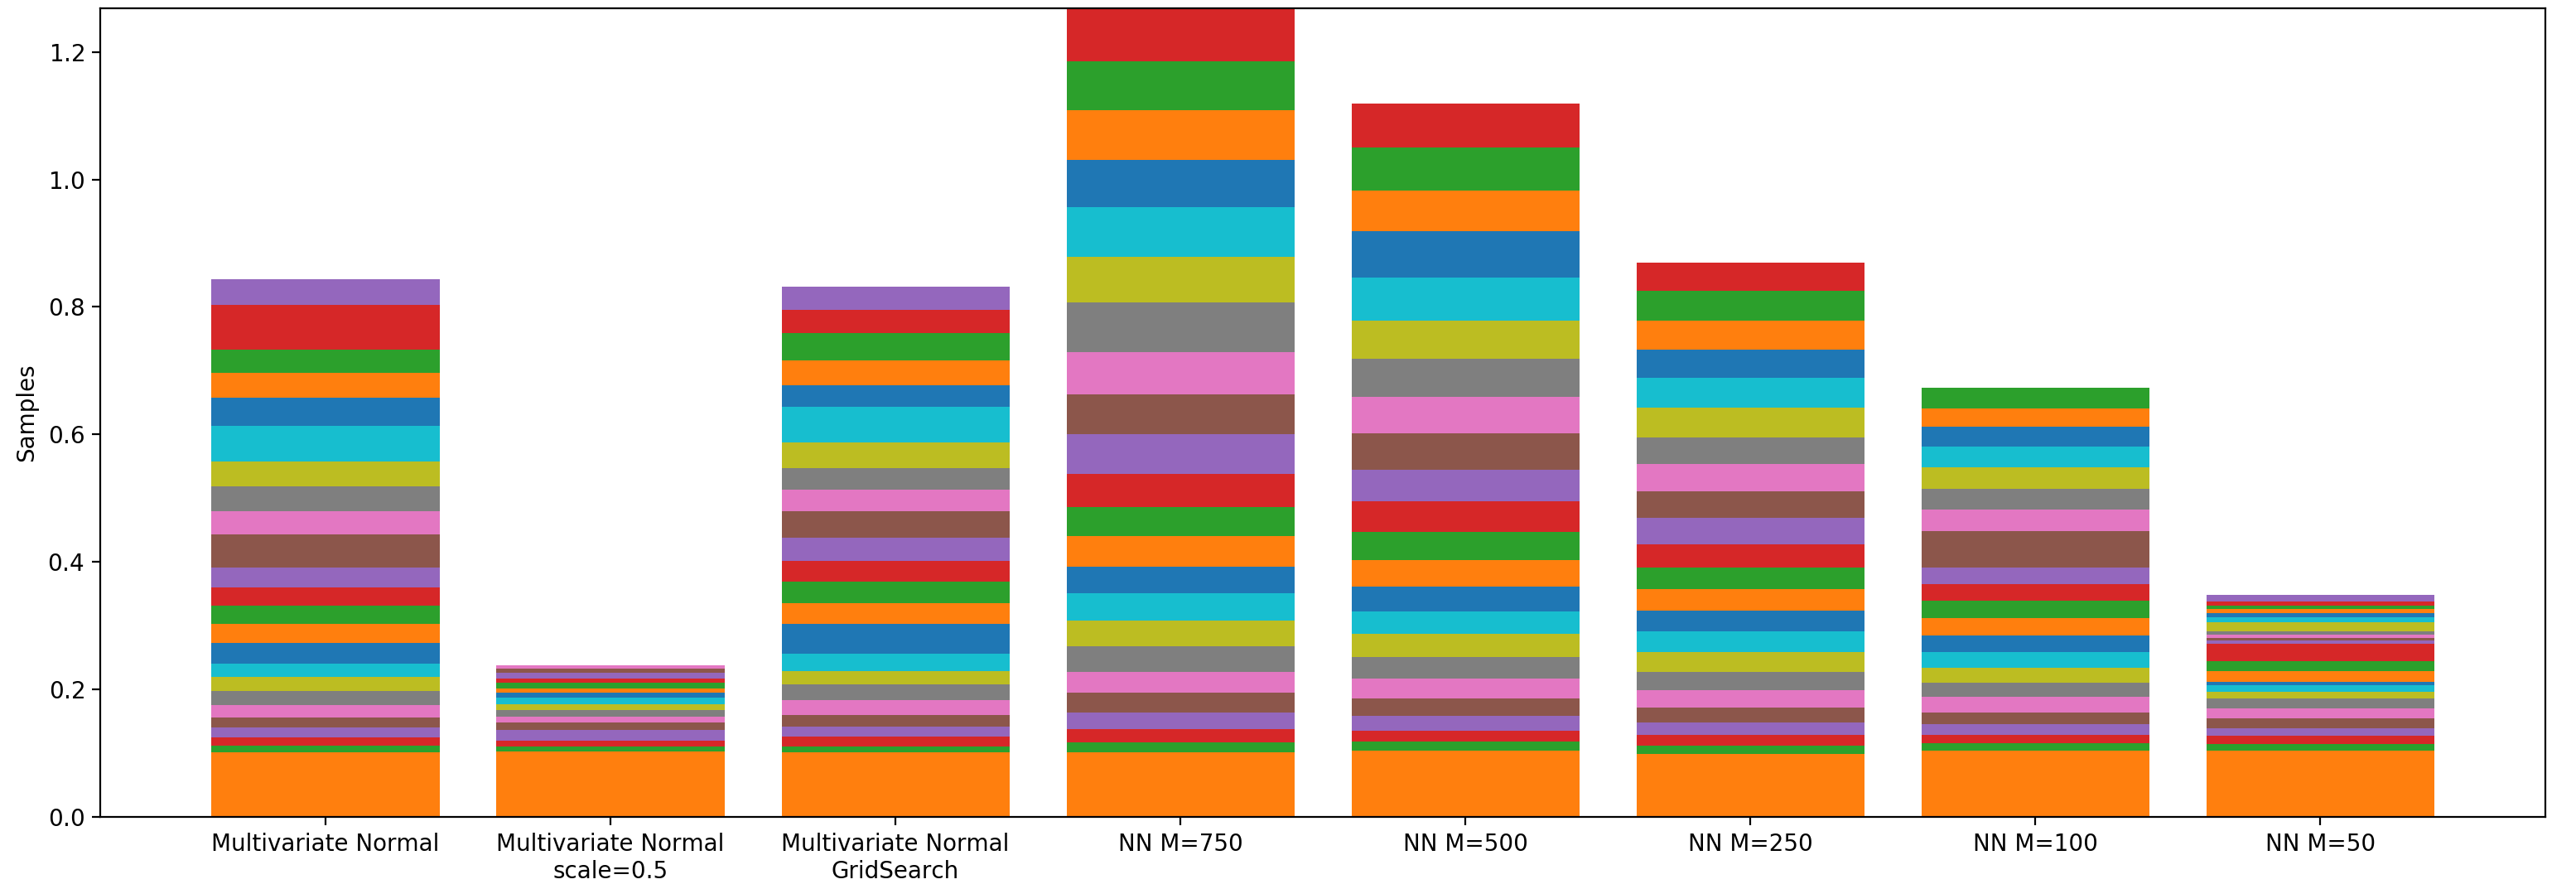
\includegraphics{fig/kernel2.png}}
    \end{center}

    \caption[Total sampling size of different kernels, using median epsilon strategy]
    {Total sampling size of different kernels, using median epsilon strategy. Different color represents different generations (bottom to top: population 1 to population 20)}
    \label{fig:kernel2}

    \begin{center}
        \resizebox{1.0\hsize}{!}{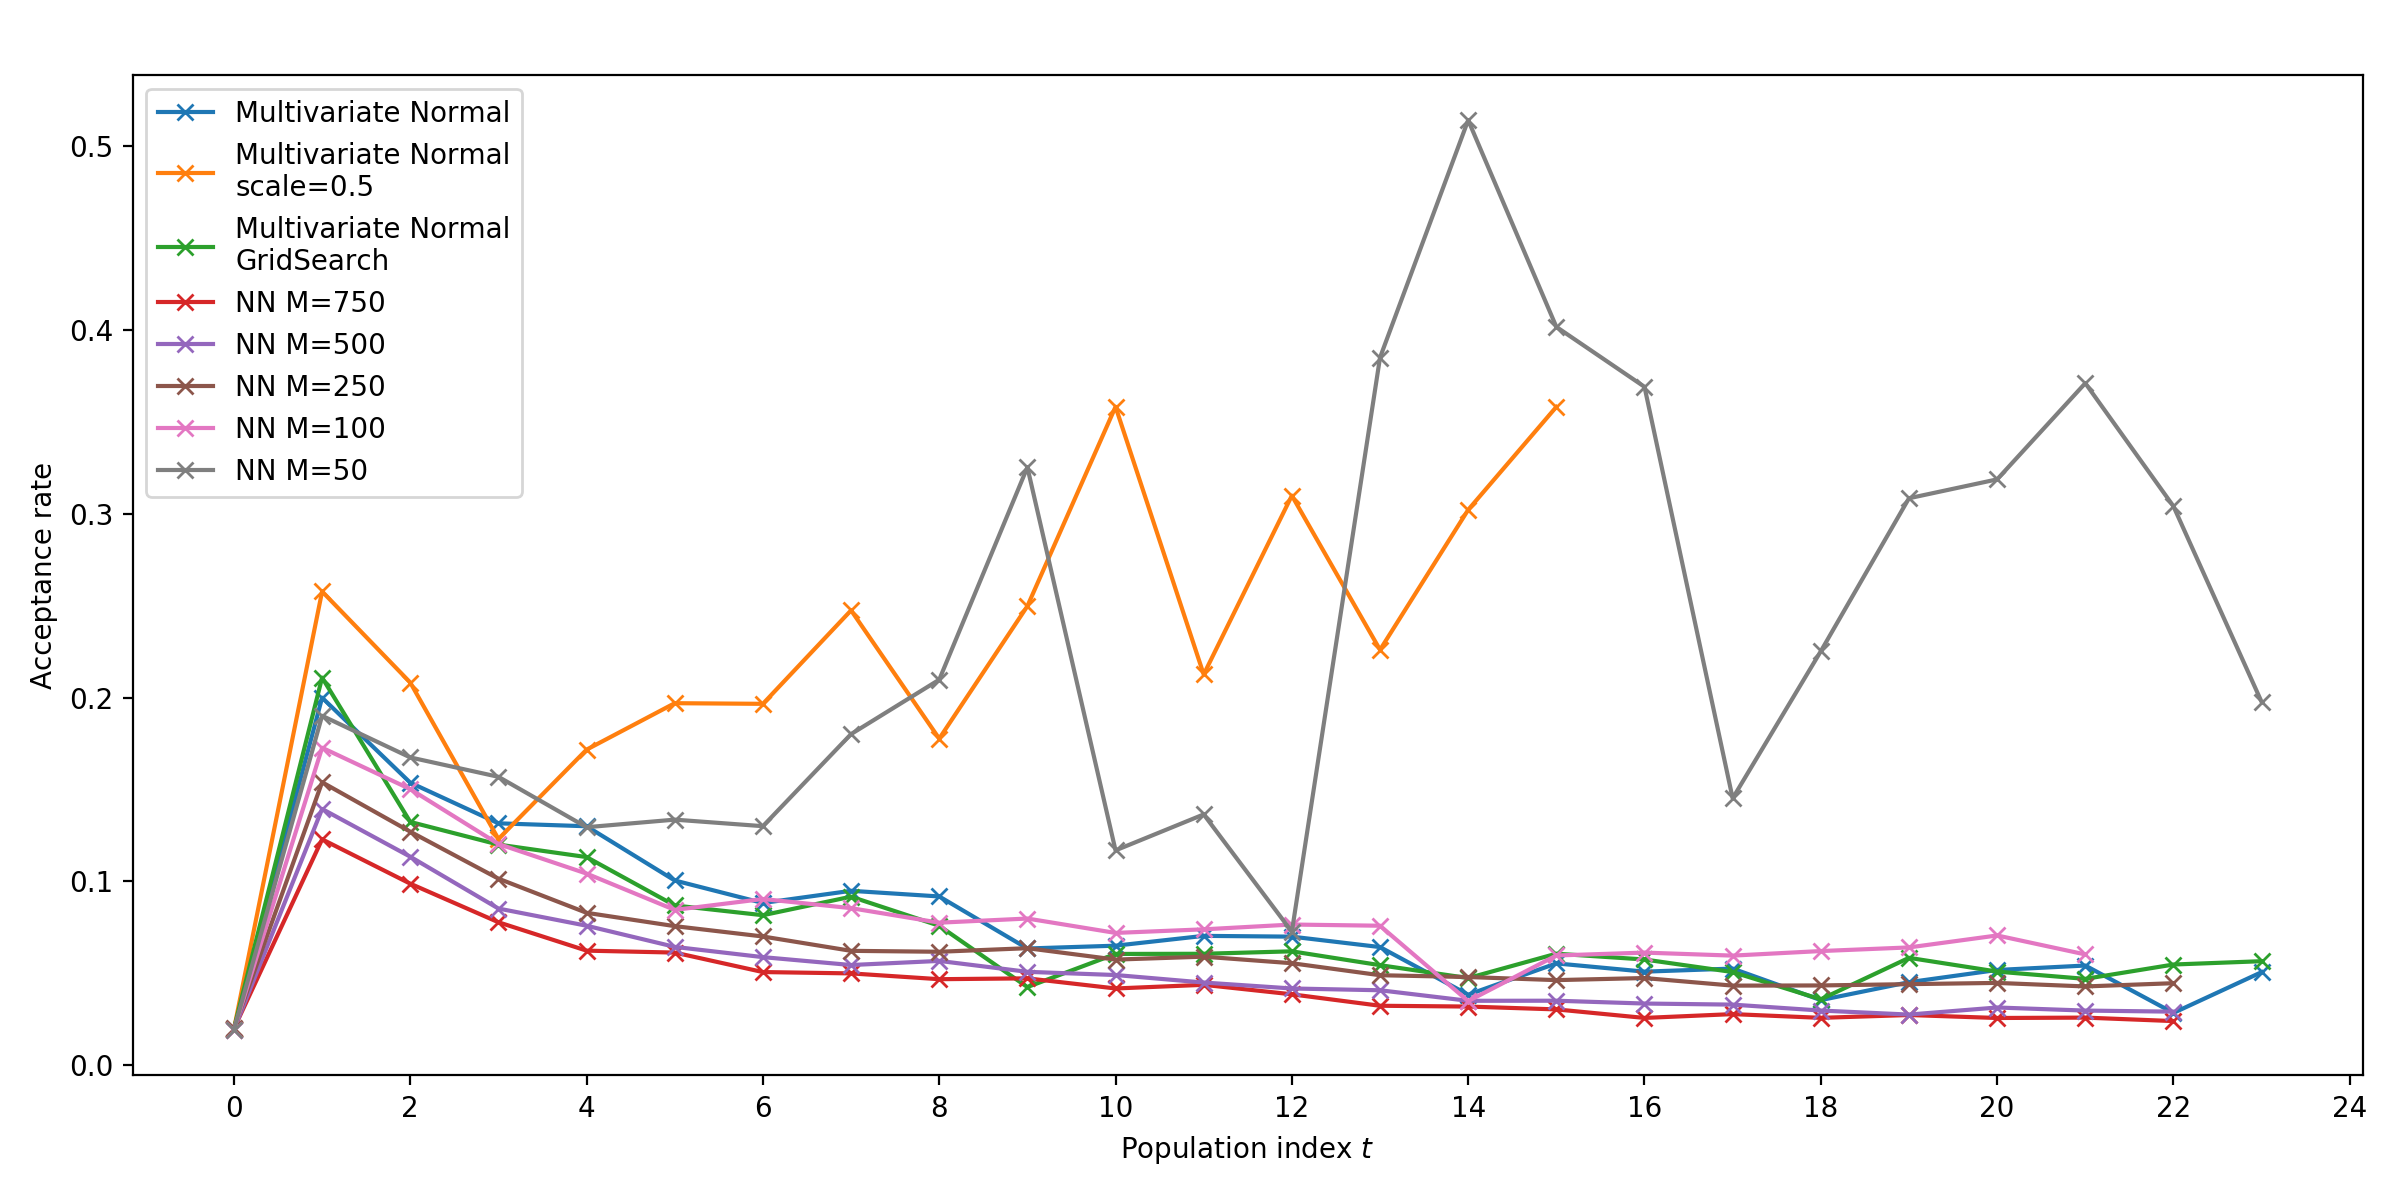
\includegraphics{fig/acceptance2.png}}
    \end{center}

    \caption[Acceptance rates of different kernels, using median epsilon strategy]
    {Acceptance rates of different kernels, using median epsilon strategy. Each population has 2000 particles}
    \label{fig:acceptance2}

\end{figure}


\section{Parameter inference and model comparison results}

\begin{figure}[H]

    \begin{center}
        \resizebox{1.0\hsize}{!}{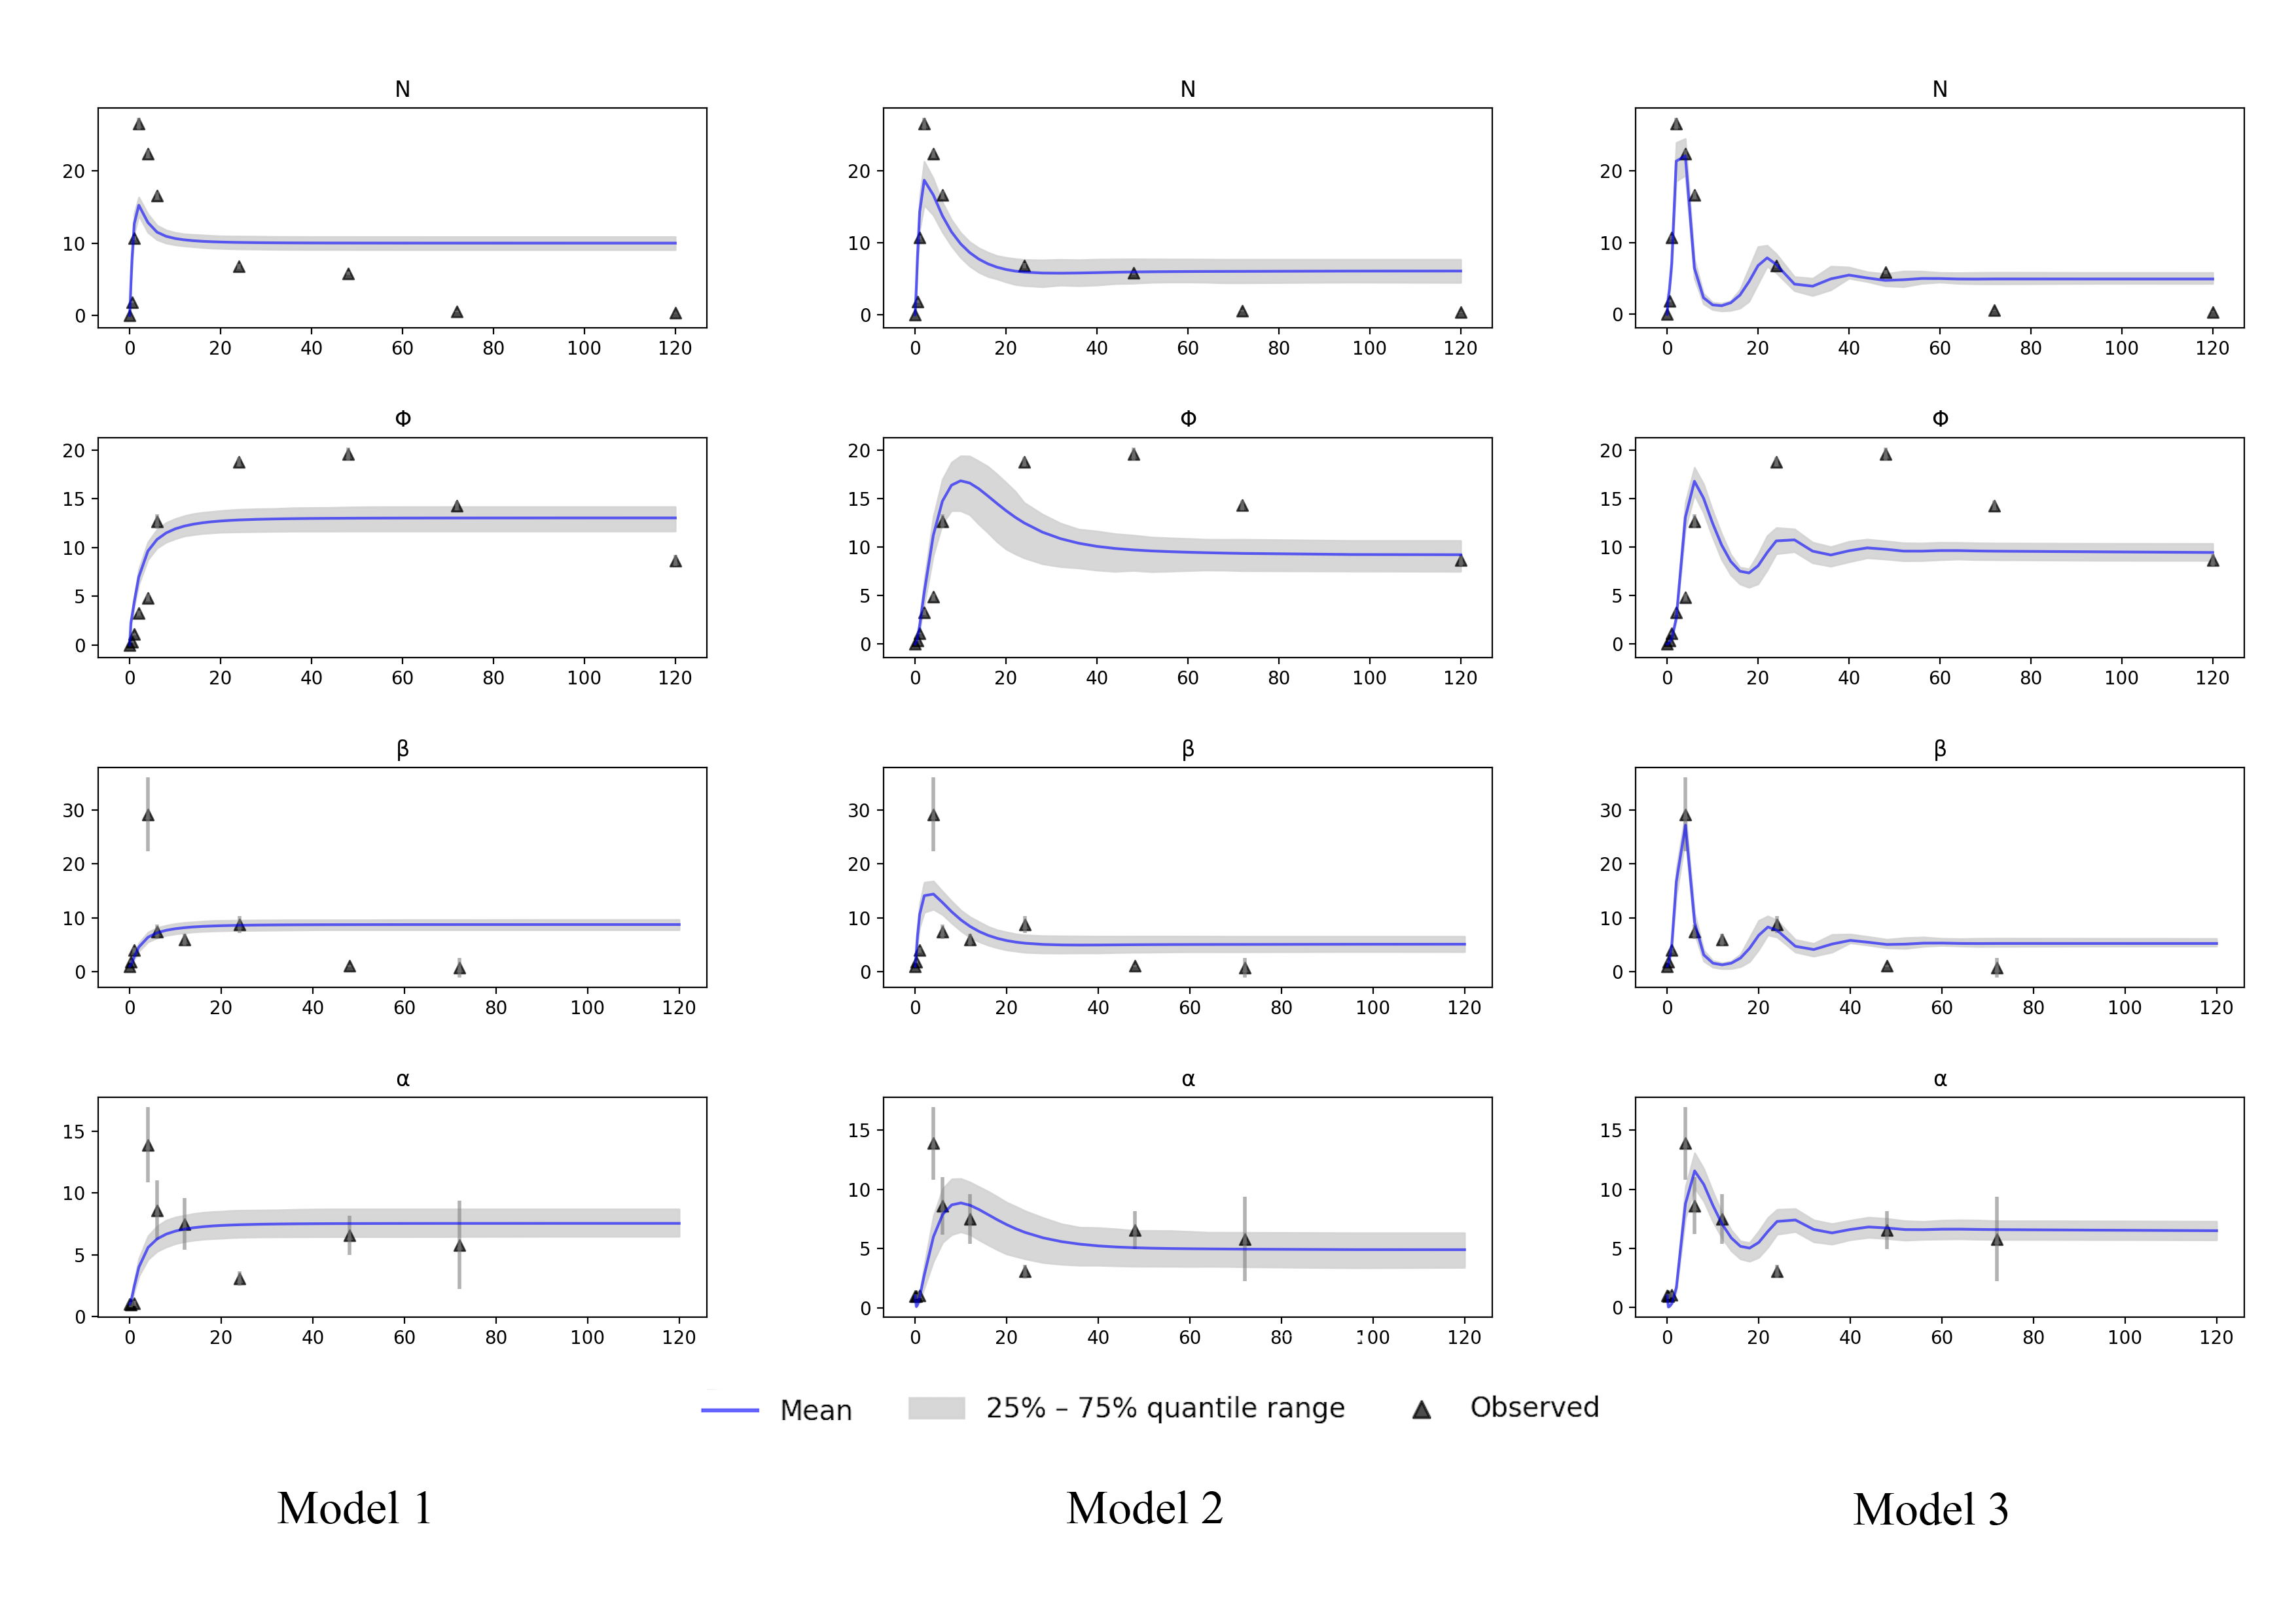
\includegraphics{fig/resultCurve_uni.png}}
    \end{center}

    \caption{Total sampling size}
    \label{fig:resultCurve_uni}


\end{figure}

\begin{figure}[ht]
    \begin{center}
        \resizebox{1.0\hsize}{!}{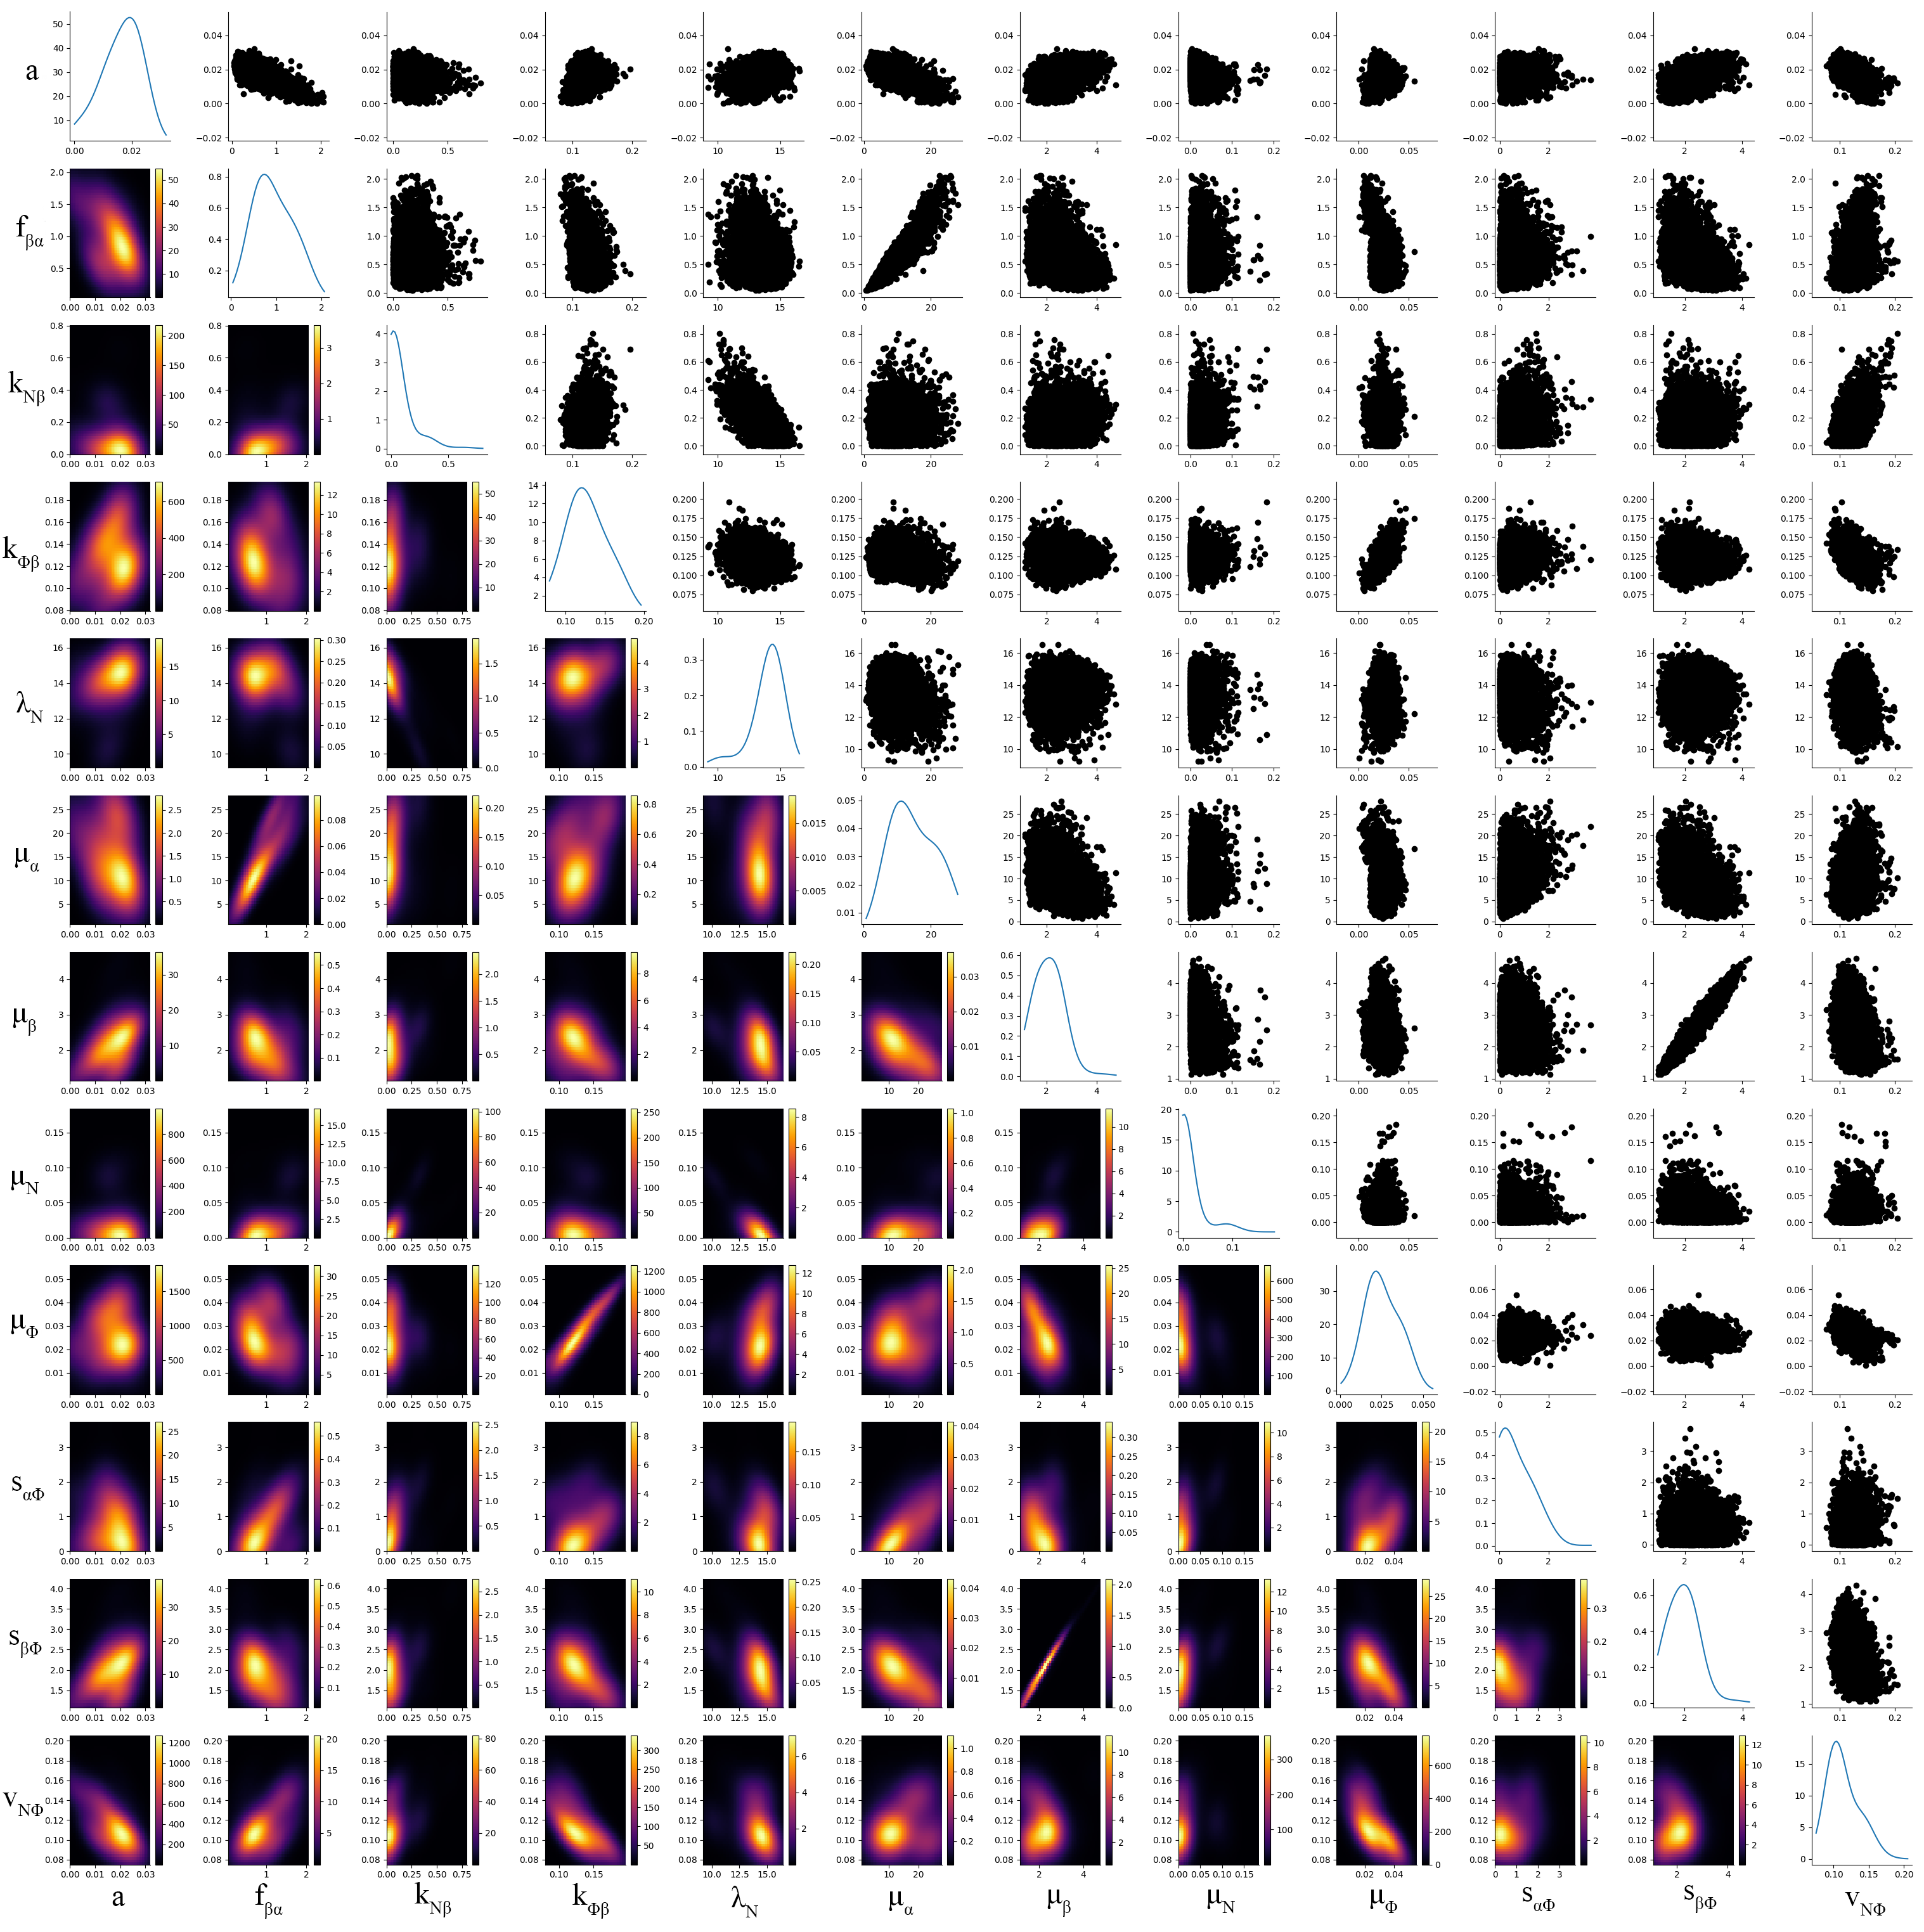
\includegraphics{fig/inferno5.png}}
    \end{center}
    \caption[Joint density distribution of each parameter pair]%
    {Joint distribution of each parameter pair. MORE DESCRIPTION}
    \label{fig:model5_para_joint}
\end{figure}

\begin{figure}[ht]
    \begin{center}
        \resizebox{1.0\hsize}{!}{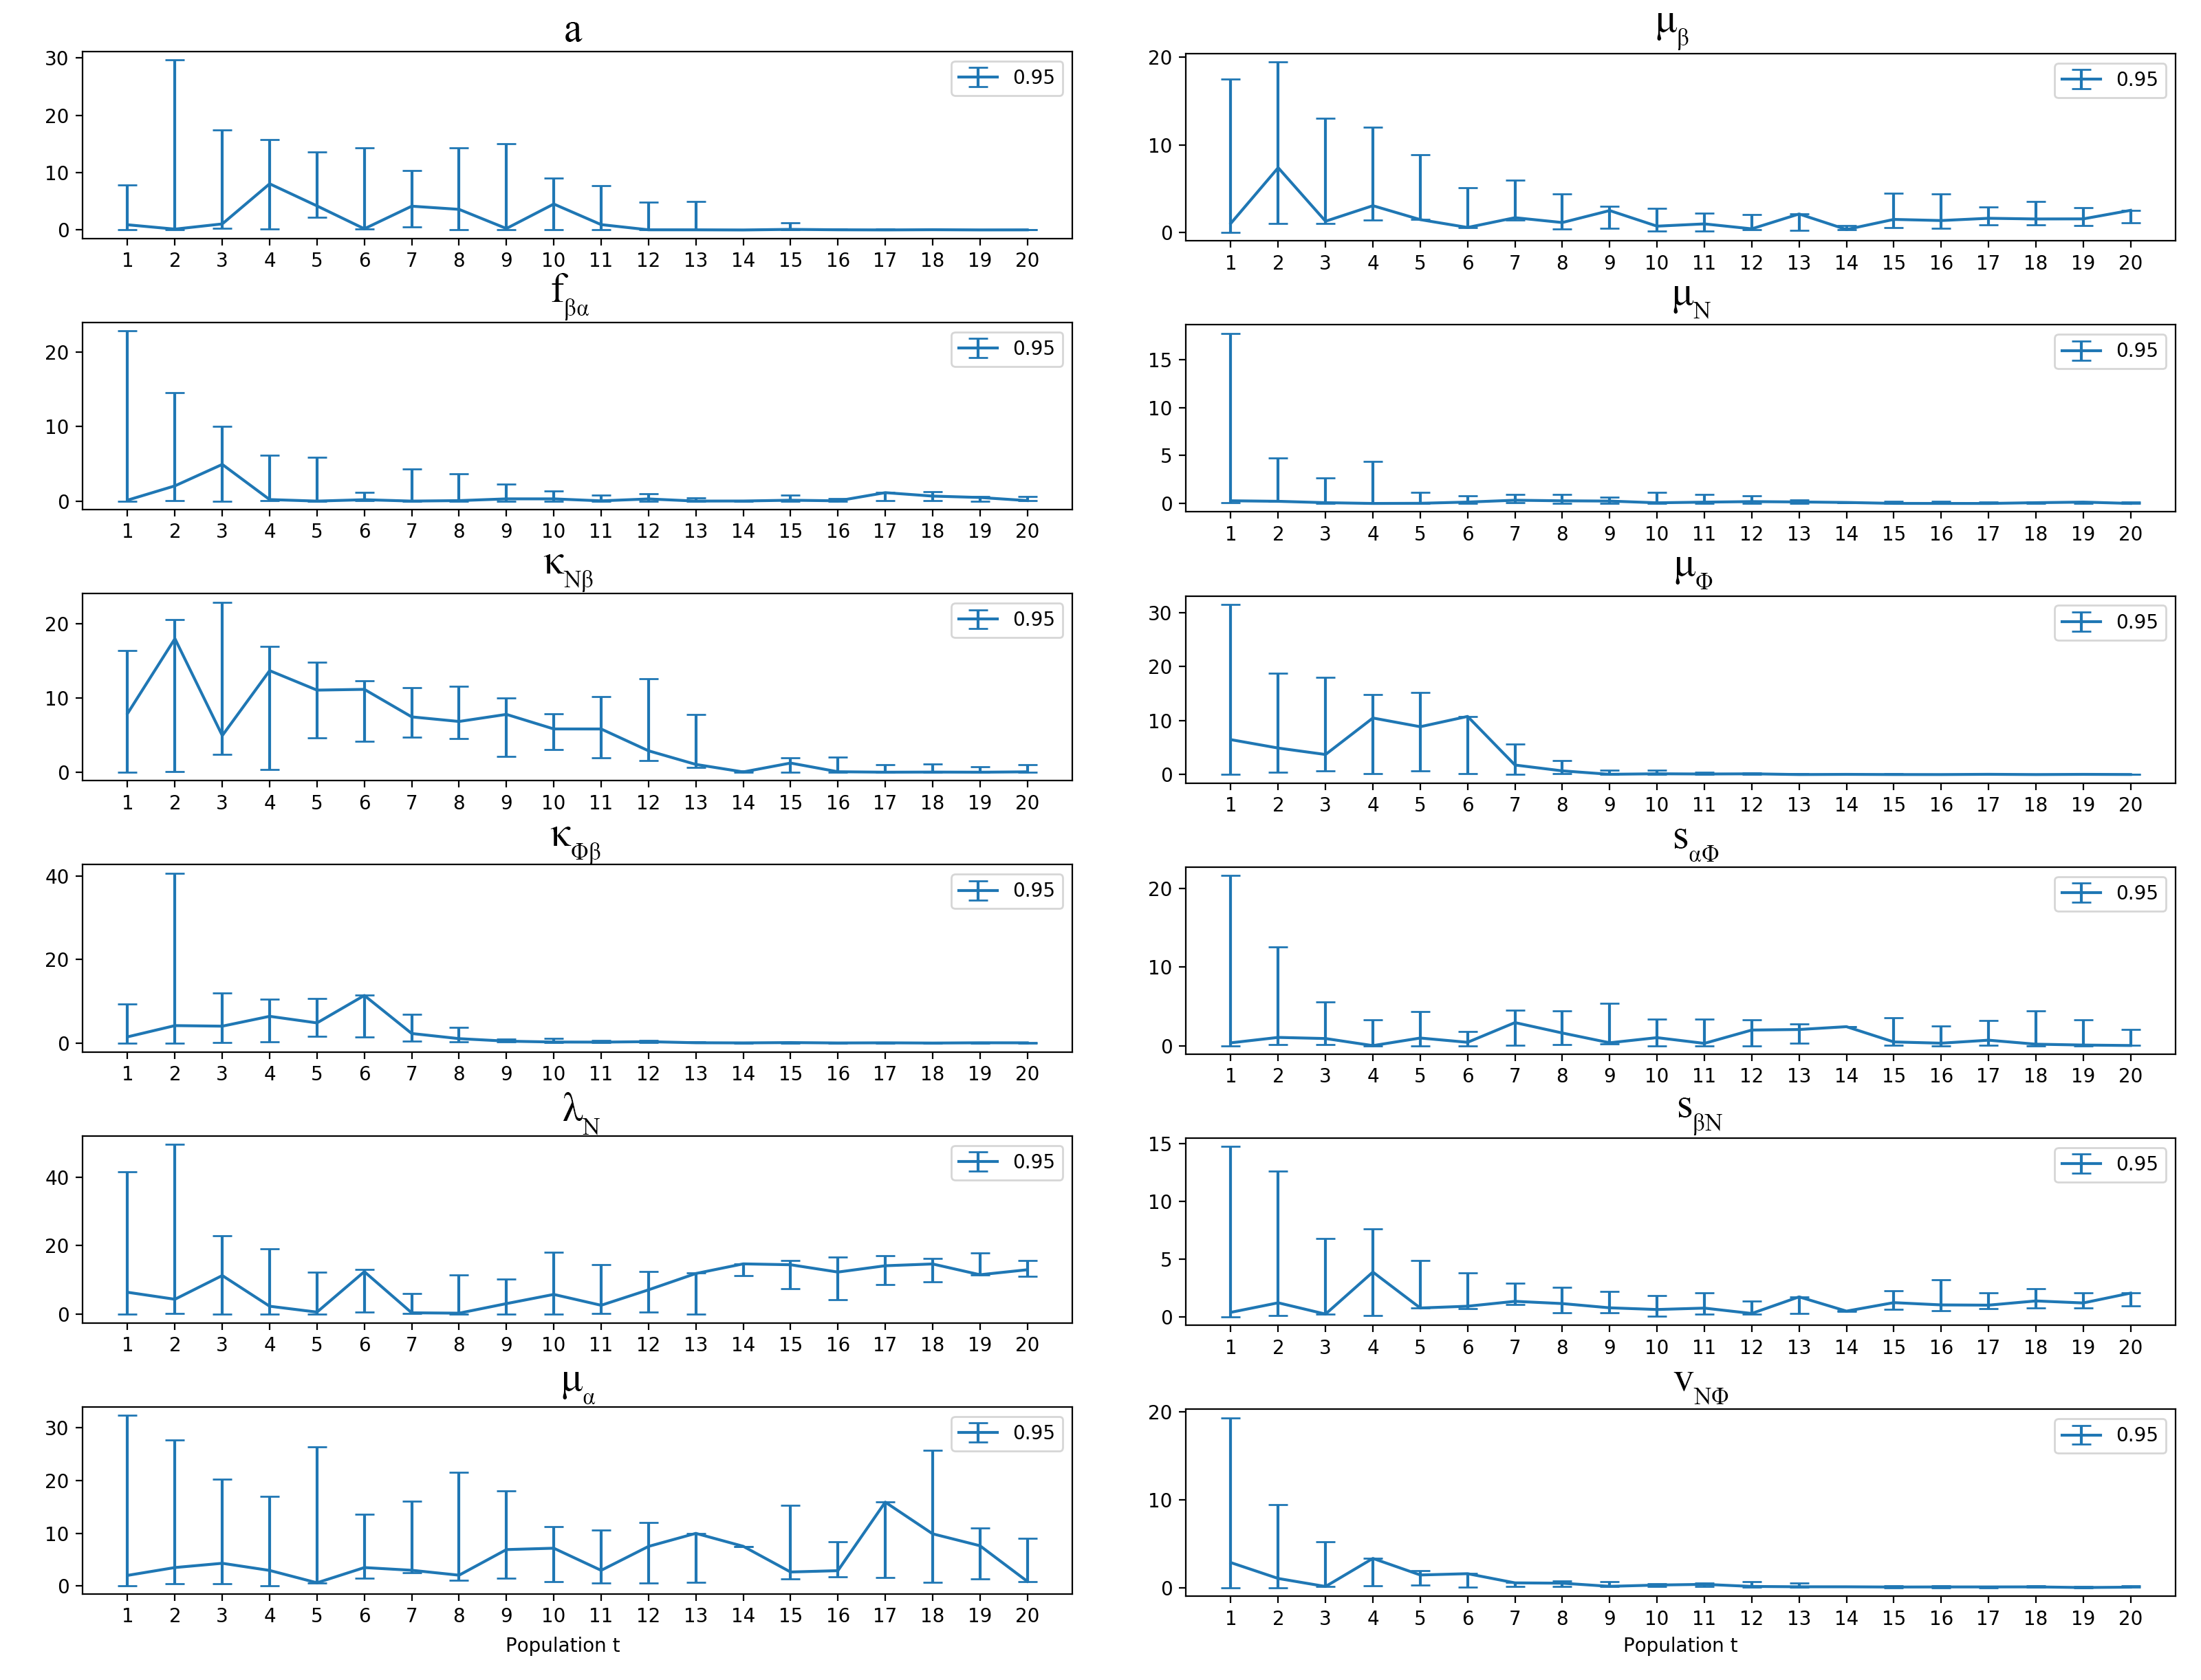
\includegraphics{fig/credible.png}}
    \end{center}
    \caption[Credible intervals of parameters in model 5]%
    {Credible intervals of parameters in model 5. MORE DESCRIPTION}
    \label{fig:credible}
\end{figure}









\bibliographystyle{ieeetr}

\bibliography{bibtex/ref}


\end{document}

